% Created 2020-10-23 Fri 18:07
% Intended LaTeX compiler: pdflatex
\documentclass[a4paper,11pt,twoside]{article}
\usepackage[utf8]{inputenc}
\usepackage[T1]{fontenc}
\usepackage{graphicx}
\usepackage{grffile}
\usepackage{longtable}
\usepackage{wrapfig}
\usepackage{rotating}
\usepackage[normalem]{ulem}
\usepackage{amsmath}
\usepackage{textcomp}
\usepackage{amssymb}
\usepackage{capt-of}
\usepackage{hyperref}
\usepackage{minted}
\IfFileExists{./resources/style.sty}{\usepackage{./resources/style}}{}
\IfFileExists{./resources/referencing.sty}{\usepackage{./resources/referencing}}{}
\addbibresource{../Resources/references.bib}
\usepackage[mode=buildnew]{standalone}
\usepackage{tikz}
\usetikzlibrary{decorations.fractals}
\usetikzlibrary{lindenmayersystems}
\author{Ryan Greenup \& James Guerra}
\date{\today}
\title{The Emergence of Patterns in Nature and Chaos Theory}
\hypersetup{
 pdfauthor={Ryan Greenup \& James Guerra},
 pdftitle={The Emergence of Patterns in Nature and Chaos Theory},
 pdfkeywords={},
 pdfsubject={},
 pdfcreator={Emacs 27.1 (Org mode 9.4)}, 
 pdflang={English}}
\begin{document}

\maketitle
\tableofcontents

 \newpage 
\section{Introduction\hfill{}\textsc{Ryan:James}}
\label{sec:orgcdb5305}
Fractals are complex shapes that often occur from natural processes, in this
report we hope to investigate the emergence of patterns and complex structures
from natural phenomena. We begin with an investigation into fractals and the
concept of dimension and then discuss links between fractal patterns and natural
processes.

\subsection{A note on Images in this report}
\label{sec:orgfc3371d}
Although the images in this document may appear to be quite small, they are high quality PNG images and one of the luxuries of PDF is that the embedded media is near lossless, so to perceive greater detail in an image it is sufficient to simply zoom in and the greater detail should be rendered. \footnote{Apparently it's also possible to embed live GIFs into PDF as well which would have been nice to do had time permitted, see for example the \texttt{Animate} package for \LaTeX \cite{CTANPackageAnimate} and \href{https://tex.stackexchange.com/questions/5396/is-there-any-way-to-include-an-animated-gif-directly}{this discussion} \cite{PdftexThereAny} generally.}

\section{Fractals}
\label{sec:org538ac7c}
\subsection{Definition of a Fractal\hfill{}\textsc{Ryan}}
\label{definition}
Benoît Mandelbrot coined the term fractal in 1975 \cite{gomoryBenoitMandelbrot19242010} and defined it in his 1982 book \emph{The Fractal Geometry of Nature} \cite[p. 15]{mandelbrotFractalGeometryNature1982} :

\begin{quote}
\emph{A fractal is by definition a set for which the Hausdorff Besicovitch dimension
strictly exceeds the topological dimension.}

\emph{Every set with a non-integer \(D\) is a fractal.} \footnote{In this quote by Mandelbrot is indicating that by the earlier definition of a
fractal, any shape (i.e. a subset of \(\mathbb{R}^{n}\) with a non-integer
dimension must be a fractal. This however is merely a sufficent, rather than a
necessary, condition of a fractal, for example the \emph{Dragon Curve} discussed in
section \ref{turtle} and the Mandlebrot set discussed at section \ref{mandlebrot-set} both
have a dimension of 2 but are clearly fractals by this definition because there
shape is constructed with a line, which has a ``topological'' dimension of 1.}
\end{quote}

The topological dimension is strictly an integer value that describes the natural dimension used to describe a shape \cite{sandersonFractalsAreTypically2017},
for example the \emph{Koch Snowflake} (shown in Figure \ref{koch-snowflake}) is composed of
just a line, so it's topological dimension would simply be 1, it's \emph{fractal
dimension} however is shown to be \(\frac{\ln\left( 4 \right)}{\ln\left( 3
\right)}\) at \eqref{eq:koch-dim} in \S\ref{topological-equivalence}.

Many authors seem to accept this earlier definition (see e.g. \cite[\S2.2]{vicsekFractalGrowthPhenomena1992} and \cite[\S2.1]{telChaoticDynamicsIntroduction2006}),
this definition however does not capture many edge-case fractals
 \cite[VII]{edgarMeasureTopologyFractal2008a} and in reprinting of \emph{The
Fractal Geometry of Nature} Mandelbrot himself commented that in hindsight it
may have been more appropriate \cite[p. 459]{mandelbrotFractalGeometryNature1982}:

\begin{quote}
\emph{to leave the term ``fractal” without a pedantic definition, to use “fractal dimension” as a generic term applicable to all the variants in Chapter 39, and to use in each specific case whichever definition is the most appropriate}.
\end{quote}

Gerald Edgar, in his 2008 book \emph{Measure, topology, and fractal geometry}
rejected this view because ``\emph{a term without a 'pedantic definition' cannot be
studied mathematically}'' \cite[VII]{edgarMeasureTopologyFractal2008a} and
presented a more robust definition in Ch. 6 of that book, it was however
accepted that the loose definition of fractal dimension is convenient and was
indeed adopted in that work.

Although reviewing the precise definition of a fractal would have been very
interesting, without a cursory knowledge of fractals generally this would have
been very time consuming and outside the scope of this report \footnote{Mandelbrot
also discussed fractals of a Euclidean and Reimannian nature,
\cite[p. 361]{mandelbrotFractalGeometryNature1982}, this again is interesting
but too specific for the broad nature of our investigation}.

Some authors simply define a fractal as a shape that \emph{shows irregularities at
all scales} \cite[p. 1]{gouyetPhysicsFractalStructures1996} and in his 2003
book, \emph{Fractal Geometry}, Facloner suggested that it is more convenient to
describe a fractal by a list of properties characteristic of such shapes \footnote{Much like the definition of life in the field of biology} because of the
difficulty in defining a fractal in a way that can encompass all edge cases and
provides the following characteristics
\cite[p. xxv]{falconerFractalGeometryMathematical2003b}:

\begin{itemize}
\item Detail at all scales
\item Cannot be described in a traditional geometric way
\item May have some form of approximate self similarity
\item Usually the fractal dimension is greater than its topological dimension
\item In many cases defined very simply, perhaps recursively
\end{itemize}

This will be the approach adopted in this report.

It's interesting to note that many authors refer to complex natural shapes as
fractals, such as coastlines (see e.g.
\cite{jiangFractalAnalysisComplexity1998,zhuFractalMechanismCoastline2002,zhongFractalPropertiesShoreline2017})
much in the spirit of Mandelbrot's paper \emph{How long is the Coastline of Britain}
\cite{mandelbrotHowLongCoast1967}, although he coined the term fractal many years
after this paper, presumably he might have had this in mind \footnote{Mandelbrot also
spent much time looking at the roughness of financial markets and so presumably
may have had that in mind as well, see e.g.
\cite{gomoryBenoitMandelbrot19242010,mandelbrotMisBehaviourMarkets2008}} when
framing the definition so this issue in clearly defining what a fractal is
appears on the surface to be a purely mathematical one (as opposed to a
practical or applied one).

The Wikipedia page on fractals \cite{Fractal2020} also points out that a
fractal is nowhere differentiable, this would be because a fractal is
nowhere smooth, which is certainly an important and distinguishing feature worth noting.

\subsection{Fractals Generally\hfill{}\textsc{James}}
\label{sec:org94d7b65}
Dimension is the main defining property of a fractal. As aforementioned above, the Hausdorff dimension is a unique number in that, if we take some shape in \(\mathbb{R}^{n}\), and the Hausdorff dimension converges to some number, then the dimension of the shape is given by that number. Otherwise, it will equal \(0\) or \(\infty\). For example, if we want to evaluate the dimension of a square and we use a 1-Dimensional shape as the cover set to calculate the Hausdorff dimension, we will get \(\infty\). On the other hand, if we do the same with a 3-Dimensional shape, we will get 0. And finally if we use a 2-Dimensional shape, the Hausdorff dimension will evaluate to 2. This same notion is important when computing the dimension of a more complex shape such as the Koch snowflake.

To define a fractal, we must define it's dimension. Whilst some research states that a fractal has a non-integer dimension, this is not true for all fractals. Although, most fractals like the Koch snowflake do in fact have non-integer dimensions, we can easily find a counter example namely, the Mandelbrot set. The Mandelbrot set lies in the same dimension as a square, a 2-Dimensional shape. However, we give recognition to the complexity and roughness of the Mandelbrot set which clearly distinguishes itself from a square. Beneath the Mandelbrot set's complexity are exact replicates of the largest scaled Mandelbrot set, i.e a self similar shape. Furthermore, although the Mandelbrot set has an integer dimension, the self similarity and complexity is what also defines its fractal nature.

\subsection{Fractal Dimension}
\label{sec:org7676ea6}
The concept of a non-integer dimension may at first seem odd, particularly given that the familiar definition from linear algebra (concerned with the number of vectors within a basis for a vector space \cite{larsonElementaryLinearAlgebra1991}) is strictly an integer value, but in the early \(20^{\mathrm{th}}\) century mathematicians recognized the shortcomings of this definition \cite[Ch. 3]{mandelbrotFractalGeometryNature1982}.

In this section we hope to convince the reader that there is grounds for
extending the definition of dimension and as a matter of fact many definitions
for non-integer dimensions of a shape have been proposed (see generally
\cite[Ch. 39]{mandelbrotFractalGeometryNature1982} and
\cite[\S 1.3]{gouyetPhysicsFractalStructures1996}) of these the Hausdorff Dimension (and corresponding Hausdorff Measure) is
considered to be the most important and mathematically robust
\cite[p. 27]{falconerFractalGeometryMathematical2003b}, while the \emph{Box-Counting Dimension} (introduced in \S \ref{box-count-dim})
has the most practical applications in science
\cite[p. 192]{peitgenChaosFractalsNew2004}.

The Hausdorff dimension is more like counting balls than boxes and is identical
to the Box-Counting Dimension in many cases, it's more general but harder to define
\cite{sandersonFractalsAreTypically2017}, An extension to the work of this report
would be to show the mathematical connections between the Hausdorff Dimension
and box counting dimension with respect to the fractals generated and measured.


\subsubsection{Topological Equivalence\hfill{}\textsc{Ryan}}
\label{topological-equivalence}
Topology is an area of mathematics concerned with ideas of continuity through the study of figures that are preserved under homeomorphic transformations \cite{gilmoreTopologyChaosAlice2002} , where two figures are said to be homeomorphic if there is a continuous bijective mapping between the two shapes \cite[p. 105]{peitgenChaosFractalsNew2004}
.
\footnote{For further reading on this topic see \cite[p. 106]{peitgenChaosFractalsNew2004}}

So for example deforming a cube into a sphere would be homeomorphic, but deforming a sphere into a torus would not, because the the surface of the shape would have to be compromised to achieve that.

Historically, as mentioned in \S \ref{definition}, the concept of dimension was a difficult problem with a tenuous
definition.  Although an intuitive definition related the dimension of a shape to
the number of parameters needed to describe that shape, this definition is not
sufficient to be preserved under a homeomorphic transform.

Consider the Koch fractal and snowflake in Figures \ref{koch-line} and \ref{koch-snowflake}, at each iteration (\(n\)) the perimeter is given by \(p_{n}= \left(\frac{4}{3} \right)p_{n-1}\) and the number of edges by \(N_{n}\):



\begin{align}
N_{n} &= N_{n-1} \cdot 4 \\
&= 3 \cdot 4^{n}
\end{align}

If the length of any individual side was given by \(l\) and scaled by some value \(s\) then the length of each individual edge would be given by:

\begin{align}
l = \frac{s \cdot l_{0}}{3^{n}}
\end{align}

The total perimeter would be given by:

\begin{align}
p_{n} &= N_{n} \times l \\
&= 3\cdot 4^{n} \times \frac{s \cdot l_{o}}{3^{n}} \\
&= 3 \cdot s \cdot  l_{0} \left( \frac{4}{3} \right)^{n}\\
 \implies p_{n} \cdot s & \propto \left(\frac{4}{3}\right)^{n}\\
& \implies  n = \frac{\log\left( 4 \right)}{\log\left( 3 \right)} \approx 1.26 \label{eq:koch-dim}
\end{align}

This means that if the Koch Snowflake is scaled by any factor, the resulting perimeter of the snowflake will not be linearly proportional to the scaling factor, as would be the case with an ordinary shape such as a square or a circle, it will instead by proportional to 1.26, this should hopefully motivate the need to more clearly define both the concept of measure (in this case the perimeter \footnote{Grant Sanderson equates the measure of a fractal as analogous to mass, which is a very helpful way comparison \cite{sandersonFractalsAreTypically2017}}) and dimension.

To clarify the Koch snowflake, is defined such that there are no edges, every point on the ``curve'' is the vertex of an equilateral triangle, this shape has no smooth edges.

See \cite[p. 414]{strogatzNonlinearDynamicsChaos2015} and \cite[\S 5.4]{baderSpacefillingCurvesIntroduction2013} for further reading on the self similar dimension of the \emph{Koch Snowflake}.

This approach of considering the scaling factor of a deterministic fractal is
known as the similarity dimension \cite[p.
413]{strogatzNonlinearDynamicsChaos2015} and should be equal to the Hausdorff and box counting dimensions for most
fractals. For fractals that aren't so obviously self similar it won't be
feasible however \cite[p. 393]{liIntegrationFuzzyLogic2006}, for example with
the Julia Set \footnote{It is indeed shown to be
mostly constant at all scales in section \S} or the outline of a coastline it is not immediately clear if the
the dimension would be constant at all scales



\begin{figure}[htbp]
\centering
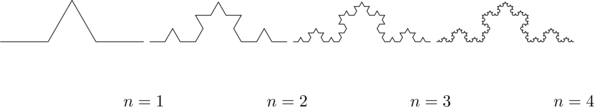
\includegraphics[width=9cm]{media/tikz/Koch_line.png}
\caption{\label{koch-line}Progression of the Koch Snowflake}
\end{figure}

\begin{figure}[htbp]
\centering
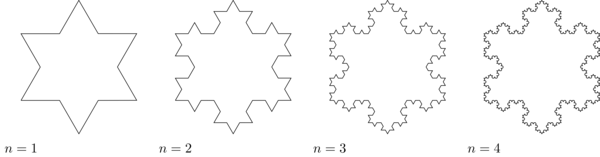
\includegraphics[width=9cm]{media/tikz/Snowflake.png}
\caption{\label{koch-snowflake}Progression of the Koch Snowflake}
\end{figure}

\subsubsection{Hausdorff Measure\hfill{}\textsc{Ryan}}
\label{hausdorff-measure}
The Hausdorff dimension depends first on a rigorous definition of measure, this is distinct from the box counting approach in that it is more mathematically rigorous, it is however complex and in practice this report will be concerned with implementing the box counting dimension. \footnote{See \S \ref{haus-resource} for further reading.}

\begin{wrapfigure}{l}{0.5\textwidth}
\centering
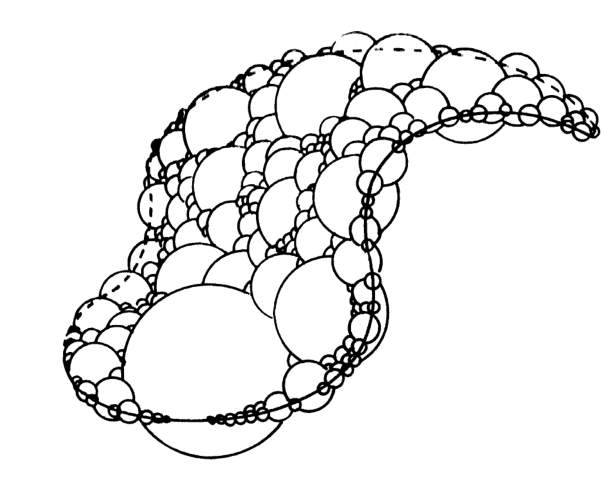
\includegraphics[width=0.38\textwidth]{media/edgar_181_of_292.png}
\caption{\label{fig:ball-covering}The Hausdorff Measure of an arbitrary surface approximated by the cross section of balls with diameter \(< \delta\), this is reproduced from \emph{Measure, Topology and Fractal Geometry} \cite[p. 166]{edgarMeasureTopologyFractal2008a}.}
\end{wrapfigure}

Let \(F\) be some arbitrary subset of euclidean space \(\mathbb{R}^n\), \footnote{A subset of euclidean space could be interpreted as an uncountable set containing all points describing that region}

Let \(U\) be a subset of euclidean space \(\mathbb{R}^{n}\) such that the diameter is defined as the greatest distance between any of the points:

\[
\left\lvert U \right\rvert = \mathrm{sup}\left(\left\{ \left\lvert x- y \right\rvert \enspace : \enspace x,y \in U\right\}  \right)
\]

Consider a collection of these sets,

\[
G = \left\{U_i: i \in \mathbb{Z}^{+}\right\}
\]

such that each element has a diameter less than \(\delta\).


The motivating idea is that if the elements of \(G\) can be laid on-top of
\(F\) then \(G\) is said to be a \(\delta\) -cover of \(F\), more rigorously, \(G\) is a \(\delta\)-cover of \(F\) if: \footnote{Falconer defines this as \(\bigcup_{i=1}^{\infty}\) \cite[\S 2.1]{falconerFractalGeometryMathematical2003b},
presumably treating any index value greater than the cardinality of the set as \(\emptyset\), this is particularly ambiguous and we have avoided it, an alternative way to present that might be \(\bigcup^{\#G}_{i=0}\) where \(\#G\) denotes the cardinality or \(G\) (or \(\infty\) if it is uncountable). The use of \(\#\square\) to denote cardinality was introduced by Knuth in \emph{Concrete Mathematics} \cite{grahamConcreteMathematicsFoundation1994} and is convenient in that it avoids any ambiguity  with diameter (\(\left\lvert \square \right\rvert\)).}

\begin{align}
    F \subset \bigcup_{U\in B} \left( U \right) \quad :\quad 0 \leq \left\lvert U \right\rvert \leq \delta \label{eq:hausdorff-covering}
\end{align}



An example of this covering is provided in Figure \ref{hausdorff-covering}, in that example the figure on the right is covered by squares, which each could be an element of \(\{U_{i}\}\), it is important to note, by this definition, that the shapes represented by \(U\) could be any arbitrary figure \cite[\S 2.1]{falconerFractalGeometryMathematical2003b} the size of which may vary in size so long as the diameter is less than \(\delta\).


So for example:

\begin{itemize}
\item \(F\) could be some arbitrary 2D shape, and \(U_{i}\) could be
a collection of identical squares, OR

\item \(F\) could be the outline of a coastline and \(U_{i}\) could be a set of circles, OR

\item \(F\) could be the surface of a sheet and \(U_{i}\) could be a set of spherical balls as shown in Figure \ref{fig:ball-covering}

\begin{itemize}
\item Some authors suggest that the Hausdorff Measure is concerned primarily with round covering objects (see e.g. \cite{sandersonFractalsAreTypically2017}), this is well illustrated by Figure \ref{fig:ball-covering}, however in truth it is merely more convenient to use round shapes for most fractals.

\item The use of balls is a simpler but equivalent approach to the theory \cite[\textsection 2.4 ]{falconerFractalGeometryMathematical2003b} because any set of diameter \(r\) can be enclosed in a ball of radius \(\frac{r}{2}\) \cite[p. 166]{edgarMeasureTopologyFractal2008}
\end{itemize}

\item \(F\) could be a more abstracted figure like Figures \ref{hausdorff-covering} or \ref{abstract-shape}  and \(\{U_{i}\}\) a collection of various different lines, shapes or 3d objects.
\end{itemize}

The Hausdorff measure is concerned with only the diameter of each element of \(\{U_{i}\}\) and considers \(\sum_{U \in G} \left[\left\lvert U\right\rvert^{s}\right]\) where each element \(U\in G\) is arranged so as to minimize the value of the summation \cite[p. 27]{falconerFractalGeometryMathematical2003b}
, the \(\delta\)-Hausdorff is hence defined, for various dimensions \(s\):

\begin{align}
\mathcal{H}^s_{\delta}\left( F \right)= \inf \left\{ \sum_{U\in G}   \left\lvert U_i \right\rvert^s \enspace : \enspace  \left\{U_i\right\} \text{ is a } \delta \text{-cover of } F \right\}, \quad \delta, s > 0 \label{eq:delta-measure}
\end{align}

The value of \(s\) can be different regardless of the dimension of \(F\), for example if \(F\) was an arbitrary 2D shape the value of \(\mathcal{H}_{\delta}^{2}\left(F\right)\)
is equivalent to considering the number of shapes \(U\in G\) (e.g. boxes, discs etc.), of
diameter \(\leq \delta\) that will cover over a shape as shown in Figure
\ref{hausdorff-covering}, the delta Hausdorff measure
\(\mathcal{H}^{2}_{\delta} \left(F\right)\) will be the area of the boxes when
arranged in such a way that minimizes the area.

As \(\delta\) is made arbitrarily small \(\mathcal{H}_{\delta}^{s}\) will approach some limit, in the case of Figures \ref{hausdorff-covering}  and \ref{abstract-shape} the value of \(\mathcal{H}^{2}_{\delta}\) will approach the area of the shape as \(\delta \rightarrow 0\) and so the \(s^{th}\) dimensional Hausdorff measure is given by:

\begin{align}
\mathcal{H}^{s} = \lim_{\delta \rightarrow 0}\left( \mathcal{H}^{s}_{\delta} \right) \label{eq:limit-haus}
\end{align}

This is defined for all subsets of \(\mathbb{R}^n\) for example the value of  \(\mathcal{H}^{2}\) corresponding to Figure \ref{abstract-shape} will be limit that boxes would approach when covering that area, which would be the area of the shape (\(4\times 1^2 + 4\times \pi\times \frac{1}{2^2} + \frac{1}{2}\times 1 \times \sin{\frac{\pi}{3}}\)).





\begin{wrapfigure}{l}{0.5\textwidth}
\centering
\includesvg[width=0.38\textwidth]{notes/HaussDorf_Dim_Ink}
\caption{\label{hausdorff-covering}The blue outline corresponds to some \(F \subset \mathbb{R}^{2}\), covered by various grey objects, each of which represent an element from the set \(U_{i}\). The grey shapes all have a diameter less than \(\delta\) and so this  \(\bigcup \left[U_{i}\right]\) would be a \(\delta\)-covering of \(F\).}
\end{wrapfigure}




\paragraph{Lower Dimension Hausdorff Measurements}
\label{sec:orga635e15}
\subparagraph{Examples}
\label{sec:org7a412f0}
Consider again the example of a 2D shape, the value of \(\mathcal{H}^{1}\) would still be defined by \eqref{eq:delta-measure}, but unlike \(\mathcal{H}^{2}\) in \S \ref{hausdorff-measure} the value of \(\left\lvert U_i \right\rvert^1\) would be considered as opposed to \(\left\lvert U_i \right\rvert^2\) (i.e. the diameter as opposed to the diameter squared).

As \(\delta\) is made arbitrarily small the boxes \footnote{Even though \(U\) may contain a variety of shapes, \eqref{eq:delta-measure} is concerned only with the power of there diameter, so in this sense the limit is concerned only with boxes corresponding to the diameter of the elements of \(U\)} that cover the shape are made also to be arbitrarily small. Although the area of the boxes must clearly be bounded by the shape of \(F\), if one imagines an infinite number of infinitely dense lines packing into a 2D shape with an infinite density it can be seen that the total length of those lines will be infinite and so the limit in \eqref{eq:limit-haus} will increase without bound.

To build on that same analogy, another way to imagine this is to pack a 2D shape with straight lines, the total length of all lines will approach the same value as the length of the lines of the squares as they are packed infinitely densely. Because lines cannot fill a 2D shape, as the density of the lines increases, the overall length will increase without bound.

This is consistent with fractals as well, consider the Koch snowflake introduced in section \ref{topological-equivalence} and shown in Figure \ref{koch-line}, the dimension of this shape, as shown in \S \ref{topological-equivalence} is greater than 1, and the number of lines necessary to describe that shape is also infinite because every point of the ``curve'' is a point of an equilateral triangle.

\subparagraph{Formally}
\label{sec:org043ec38}
If the dimension of \(F\) is less than \(s\), the Hausdorff Measure will be given by:

\begin{align}
\mathrm{dim}\left(  F \right ) < s \implies \mathcal{H}^{s} \left( F \right)  = \infty
\end{align}

\paragraph{Higher Dimension Hausdorff Dimension}
\label{sec:orgad11cfb}


For small values of \(s\) (i.e. less than the dimension of  \(F\)), the value of \(\mathcal{H}^s\)  will be \(\infty\).

Consider some value \(s\) such that the Hausdorff measure is not infinite, i.e. values of \(s\):

\[
\mathcal{H}^s = L \in \mathbb{R}
\]

Consider a dimensional value \(t\) that is larger than  \(s\) and observe that:

\begin{align*}
0<s<t  \implies   \sum_{i}  \left[ \left\lvert U_i \right\rvert^t \right] &= \sum_{i}\left[ \left\lvert U_i \right\rvert^{t- s} \cdot  \left\lvert U_i \right\rvert^s \right] \\
&\leq \sum_{i} \left[ \delta^{t - s} \cdot \left\lvert U_i \right\rvert^s  \right]    \\
&= \delta^{t- s}\sum_{i}   \left[ \left\lvert U_i \right\rvert^s \right] 									   \\
\end{align*}

Now if \(\lim_{\delta \rightarrow 0}\left[ \sum_{i}   \left\lvert U_i \right\rvert^s \right]\) is defined as a non-infinite value:

\begin{align}
    \lim_{\delta \rightarrow 0} \left( \sum_{i}   \left[ \left\lvert U_i \right\rvert^t \right]  \right) & \leq \lim_{\delta}\left( \delta^{t- s} \sum_{i}   \left[ \left\lvert U_i \right\rvert^s \right]  \right) \\
&\leq \lim_{\delta \rightarrow 0}\left( \delta^{t - s} \right) \cdot  \lim_{\delta \rightarrow 0}\left( \sum_{i} \left[ \left\lvert U_i \right\rvert^s \right]    \right) \\
&\leq 0
\end{align}

and so we have the following relationship:

\begin{align}
    \mathcal{H}^{s} \left(F\right) \in \mathbb{R}^{+}  \implies  \mathcal{H}^t\left( F \right)= 0 \quad \forall t > s \label{eq:hdfzero}
\end{align}

Hence the value of the s-dimensional \emph{Hausdorff Measure}, \(s\) is only a finite, non-zero value, when \(s = \mathrm{dim}_{H}\left( F \right)\).



\begin{figure}[htbp]
\centering
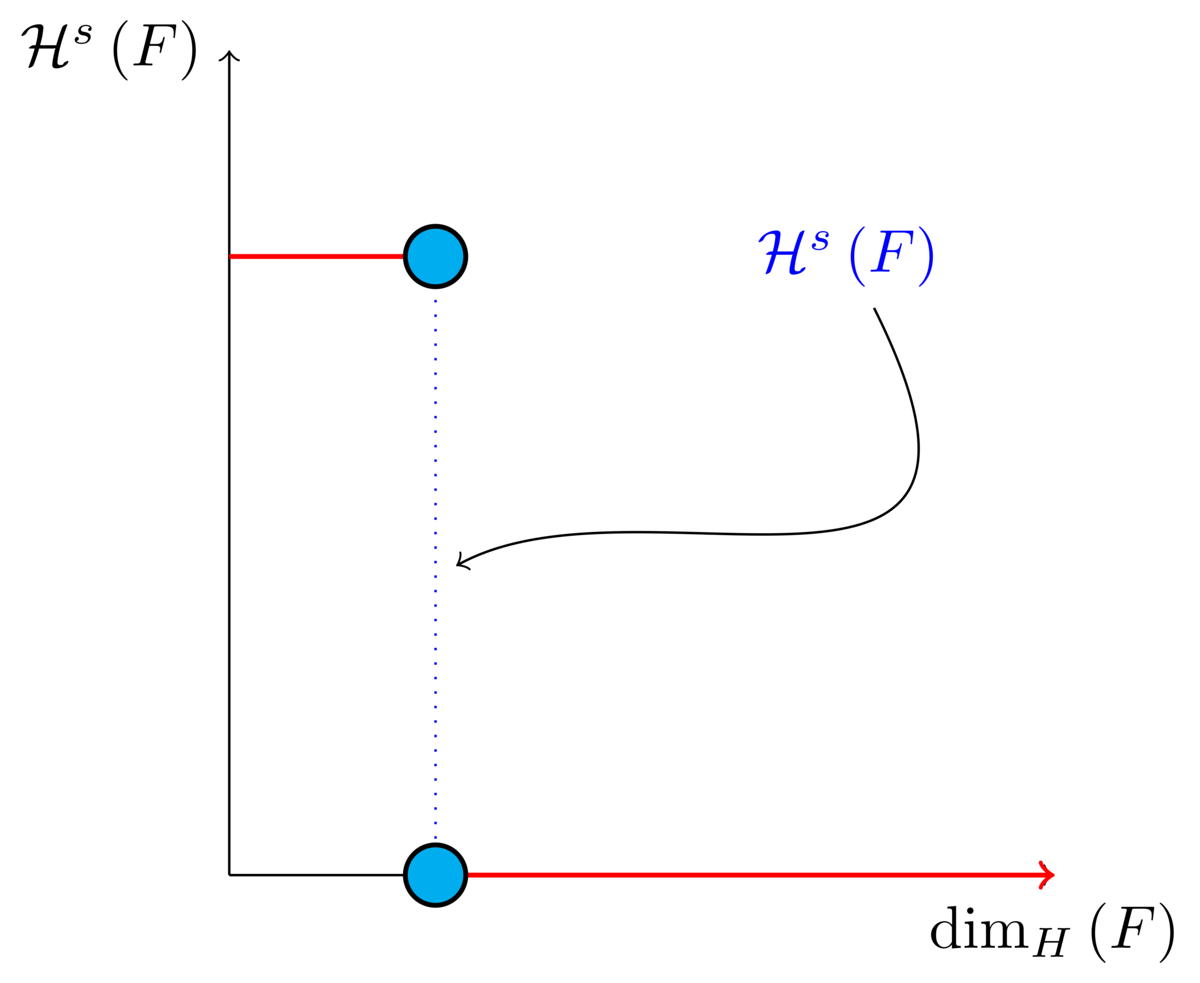
\includegraphics[width=0.85\textwidth]{media/tikz/hausdorff-dimension-plot.png}
\caption{\label{hausdorff-vals}The value of the s-dimensional \emph{Hausdorff Measure} of some subset of \emph{Euclidean space} \(F\in \mathbb{R}^{n}\) is 0 or \(\infty\) when the dimension of \(F\) is not equal to \(s\).}
\end{figure}

\subsubsection{Hausdorff Dimension\hfill{}\textsc{Ryan}}
\label{sec:org8bb3a49}

\begin{wrapfigure}{l}{0.5\textwidth}
\centering
\includesvg[width=0.28\textwidth]{media/Arbitrary-F-Shape}
\caption{\label{abstract-shape}A disconnected subset of \(\mathbb{R}^{2}\), the squares have a diameter of \(\sqrt{2}\), the circles 1 and the equilateral triangles 1.}
\end{wrapfigure}


The value \(s\) at which \(\mathcal{H}^{s}\) \eqref{eq:hdfzero} changes from \(\infty\) to 0, shown in Figure \ref{hausdorff-vals},  is the defined to be the \emph{Hausdorff Dimension} \cite[\S 2.2]{falconerFractalGeometryMathematical2003b}, it is a generalization of the idea of dimension that is typically understood with respect to ordinary figures.

\subsubsection{Box Counting Dimension\hfill{}\textsc{James}}
\label{box-count-dim}
While the Hausdorff dimension is the first formal definition to measure
the roughness of a fractal, there are several other definitions of dimension
that have stemmed from this. Namely, the box-counting dimension. The box
counting method is widely used as it is relatively easy to calculate \cite[p. 41]{falconerFractalGeometryMathematical2003b}
and in many cases is equal to the \emph{Hausdorff Dimension}  \cite[p. 11]{markpollicottFractalsDimensionTheory2005} (see generally \cite{ListFractalsHausdorff2020}).
The box-counting dimension is defined as the following from
\cite{falconerFractalGeometryMathematical2003}:

Let \(F\) be any non-empty bounded subset of \(\mathbb{R}^n\) and let \(N_\delta(F)\) be the smallest
number of sets of diameter at most \(\delta\) which can cover \(F\). The \emph{lower} and \emph{upper}
box-counting dimensions of \(F\) respectively are defined as

\begin{equation*}
    \underline{\text{dim}}_BF = \underline{\lim}_{\delta \to 0} \frac{\ln N_\delta(F)}{-\ln \delta}
\end{equation*}
\begin{equation*}
\overline{\text{dim}}_BF = \overline{\lim}_{\delta \to 0} \frac{\ln N_\delta(F)}{-\ln \delta}
\end{equation*}

When the \emph{lower} and \emph{upper} box-counting dimensions of \(F\) are equal, then

\begin{equation*}
\text{dim}_BF = \lim_{\delta \to 0} \frac{\ln N_\delta(F)}{-\ln \delta}
\end{equation*}

For example, suppose we had a square with side length 1 and we use smaller squares of side
length \(\frac{1}{\delta}\) to cover the larger square. This would mean that one side of the
large square would need \(\delta\) \(\frac{1}{\delta}\) small squares, and so to cover
the entire square, one would need \(n^2\) small squares, i.e. \(N_{\frac{1}{n}}(F) = n^2\). Now,
substituting these values into the box-counting definition, we get:

\begin{align*}
\text{dim}_BF &= \lim_{\frac{1}{\delta} \to 0} \frac{\ln(\delta^2)}{-\ln(\frac{1}{\delta})}\\
&= \lim_{\frac{1}{\delta} \to 0} \frac{\ln(\delta^2)}{\ln(\delta)}\\
&= \lim_{\frac{1}{\delta} \to 0} 2\frac{\ln(\delta)}{\ln(\delta)}\\
&= 2
\end{align*}

Which is expected, because we know that a square is a 2-Dimensional shape. We
can apply this same concept to fractals. Consider another example, the Koch
Curve, a self similar fractal which we can calculate its dimension and provide a
measure of roughness of the curve. If we take a close look at the curve progression
in Figure \ref{koch-line}, the pattern begins with one line segment and the middle third
of the line is replaced with two sides of an equilateral triangle with side length
\(\frac{1}{3}\). After this first iteration, the line segment now becomes four line
segments. Thus, if we use a square of length \(\frac{1}{3^{\delta}}\) to cover the \(\delta^{th}\)
iteration of the curve, there will be \(4^{\delta}\) line segments covered.

Let \(F\) be the Koch Curve.
\begin{align*}
\text{dim}_BF &= \lim_{\frac{1}{3^{\delta}} \to 0} \frac{\ln(4^{\delta})}{-\ln(\frac{1}{3^{\delta}})}\\
&= \lim_{\frac{1}{3^{\delta}} \to 0} \frac{\ln(4^{\delta})}{\ln(3^{\delta})}\\
&= \lim_{\frac{1}{3^{\delta}} \to 0} \frac{\ln(4)}{\ln(3)}\\
&= \frac{\ln(4)}{\ln(3)}
\end{align*}
\subsection{Generating Self Similar Fractals}
\label{gen-self-sim-frac}
In order to investigate the dimension of fractals, we intend to generate and measure a variety of figures by using of \textbf{\emph{R}} \cite{rcoreteamLanguageEnvironmentStatistical2020}, \emph{Julia} \cite{bezansonJuliaFreshApproach2017} and \emph{Python} \cite{WelcomePythonOrg}.

Self Similar fractals have a self-similar dimension and so can be used to verify an approach implemented with a programming language.
\subsubsection{Vicsek Fractal\hfill{}\textsc{Ryan}}
\label{vicsek-fractal}
The Vicsek Fractal \cite[p. 12]{vicsekFractalGrowthPhenomena1992} involves a pattern of iterating boxes, to implement this consider the process\footnote{This was actually a fractal I came up with myself only to later find that somebody already had the same idea!}:



\begin{align}
\mathbf{B} \leftarrow
   \begin{bmatrix}
       \mathbf{B} & \mathbf{Z} & \mathbf{B} \\
       \mathbf{Z} & \mathbf{B} & \mathbf{Z} \\
       \mathbf{B} & \mathbf{Z} & \mathbf{B} \\
   \end{bmatrix} \label{eq:visek-iter}
\end{align}

where:

\begin{itemize}
\item \(\mathbf{B}= \left[ 1 \right]\)
\item \(\mathbf{Z}= \left[ 0 \right]\)
\end{itemize}


\begin{wrapfigure}{l}{0.5\textwidth}
\centering
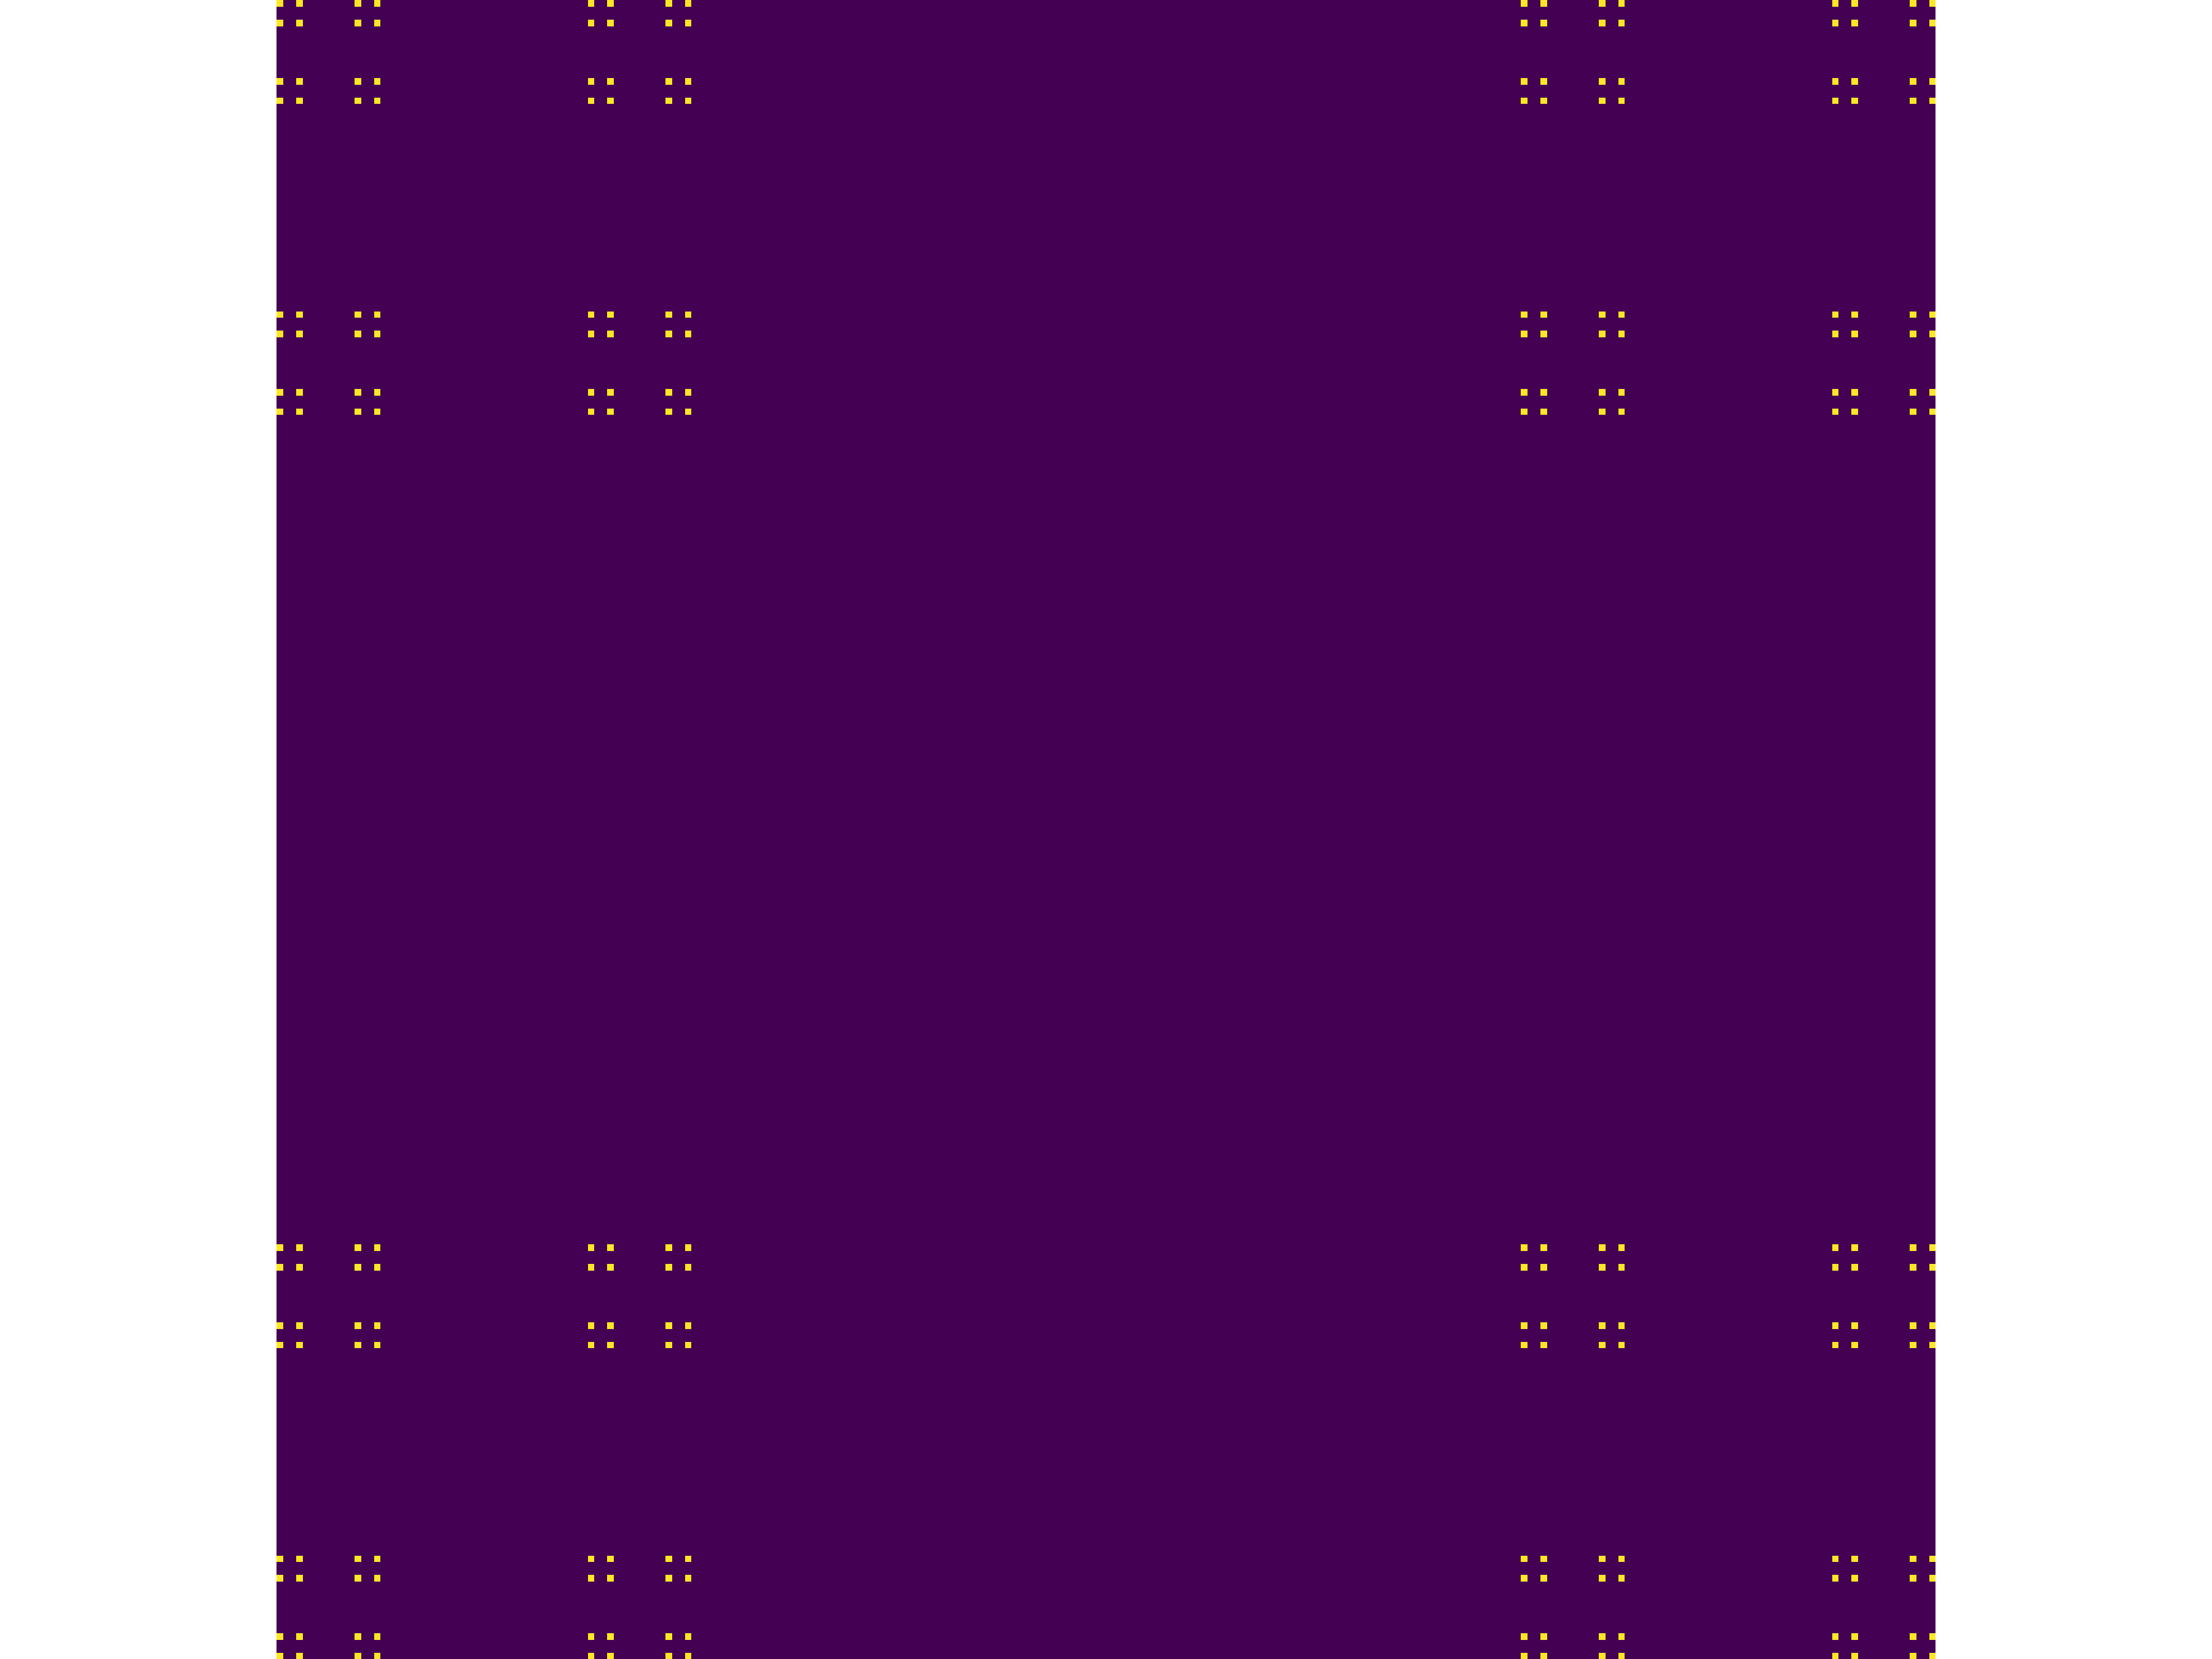
\includegraphics[width=0.38\textwidth]{media/Vicsek-Fractal.png}
\caption{\label{vicsek-fractal-julia}Vicsek fractal \cite[p. 12]{vicsekFractalGrowthPhenomena1992} (also known as the \emph{Anti-Cross-Stitch} \cite{janwassenaarCantorDust2005}) produced by listing \ref{vicsek-matrix-gen}, at each iterative step the fractal itself is ``copied'' to the four corners of itself producing this complex shape.}
\end{wrapfigure}

If this is repeated many times a matrix of values will be created, such a matrix
can be interpreted as a greyscale image and plotted as a heat-map to show the
fractal (shown in Figure ).


The iterative process shown in \eqref{eq:visek-iter} is represented as a recursive function at line 5 of listing \ref{vicsek-matrix-gen} and visualized at line 22. To measure the the dimension of this fractal a the sum of the matrix is taken to be the measure of the fractal, two fractals are generated and the change in size relative to the scale is compared and the log taken to return the value of the dimension:

\[
\mathcal{D} = \frac{s}{m_{2}/m_{1}}
\]

The recursive function begins with a 3x3 matrix, where the four corner squares
and middle square are set to 1 and the rest are set to 0, a new matrix is built
by joining together the past matrix following the rule described in \eqref{eq:visek-iter}.
The function repeats until it reaches some arbitrary set width.





At each step of the process, the number of elements of this fractal increases by
a ratio of 5 while the height increases only by a factor of 3, hence the self
similarity dimension is given by:


\begin{align}
5 &= 3^{\mathcal{D}} \nonumber \\
\implies \mathcal{D} &= \frac{\ln 5}{\ln 3} \label{eq:vic-dim-val}
\end{align}





By modifying listing \ref{vicsek-matrix-gen} alternative fractals can get also be generated like \emph{Cantor's Dust} and \emph{Sierpinski's Carpet} shown in Figures and .

Upon review this is actually a variant on the \emph{Cantor Dust} which should
actually be represented by a \(3 \times 3\) matrix:

\begin{align}
 \mathbf{B} \leftarrow
 \begin{bmatrix}
    \mathbf{B} & \mathbf{Z} & \mathbf{B} \\
    \mathbf{Z} & \mathbf{Z} & \mathbf{Z} \\
    \mathbf{B} & \mathbf{Z} & \mathbf{B} \\
\end{bmatrix}
\end{align}


and hence has the same dimension as the \emph{Vicsek Fractal} as opposed to a
dimension of 1.


\begin{listing}[htbp]
\begin{minted}[]{julia}
#------------------------------------------------------------
#--- Function -----------------------------------------------
#------------------------------------------------------------
function vicsek_matrix(ICMat, width)
    B = ICMat
    h  = size(B)[1]
    w  = size(B)[2]
    Z  = zeros(Int, h, w)
    B = [B Z B ;
         Z B Z ;
          B Z B]
    if (3*w)<width
        B = vicsek_matrix(B, width)
    end
    return B
end

#------------------------------------------------------------
#-- Plot ----------------------------------------------------
#------------------------------------------------------------
(mat = vicsek_matrix(fill(1, 1, 1), 27)) |> size
GR.imshow(mat)

#------------------------------------------------------------
#-- Similarity Dimension ------------------------------------
#------------------------------------------------------------

mat2  = vicsek_matrix(fill(1, 1, 1), 1000)
l2    = sum(mat2)
size2 = size(mat2)[1]

mat1  = vicsek_matrix(fill(1, 1, 1), 500)
l1    = sum(mat1)
size1 = size(mat1)[1]

#------------------------------------------------------------
julia> log(l2/l1)/log(size2/size1)
1.4649735207179269
julia> log(5)/log(3)
1.4649735207179269
\end{minted}
\caption{\label{vicsek-matrix-gen}Generating the Vicsek Fractal (shown in Figure \ref{vicsek-fractal-julia}) and measuring the dimension using \emph{Julia}, the measured dimension is consistent with the self similarity dimension shown in \eqref{eq:vic-dim-val}}
\end{listing}


\paragraph{Sierpinskis Carpet and Cantor's Dust}
\label{sec:org2c6e452}
By modifying the approach provided in listing \ref{vicsek-matrix-gen} other fractals
such as \emph{Sierpinski's Carpet} and \emph{Cantor's Dust} can be produced, this is
implemented in listings \ref{l-s-carpet} \ref{l-cant-dust} provided in the appendix and shown in the following figures


\phantomsection
\label{fig:square-carpet}
\begin{center}
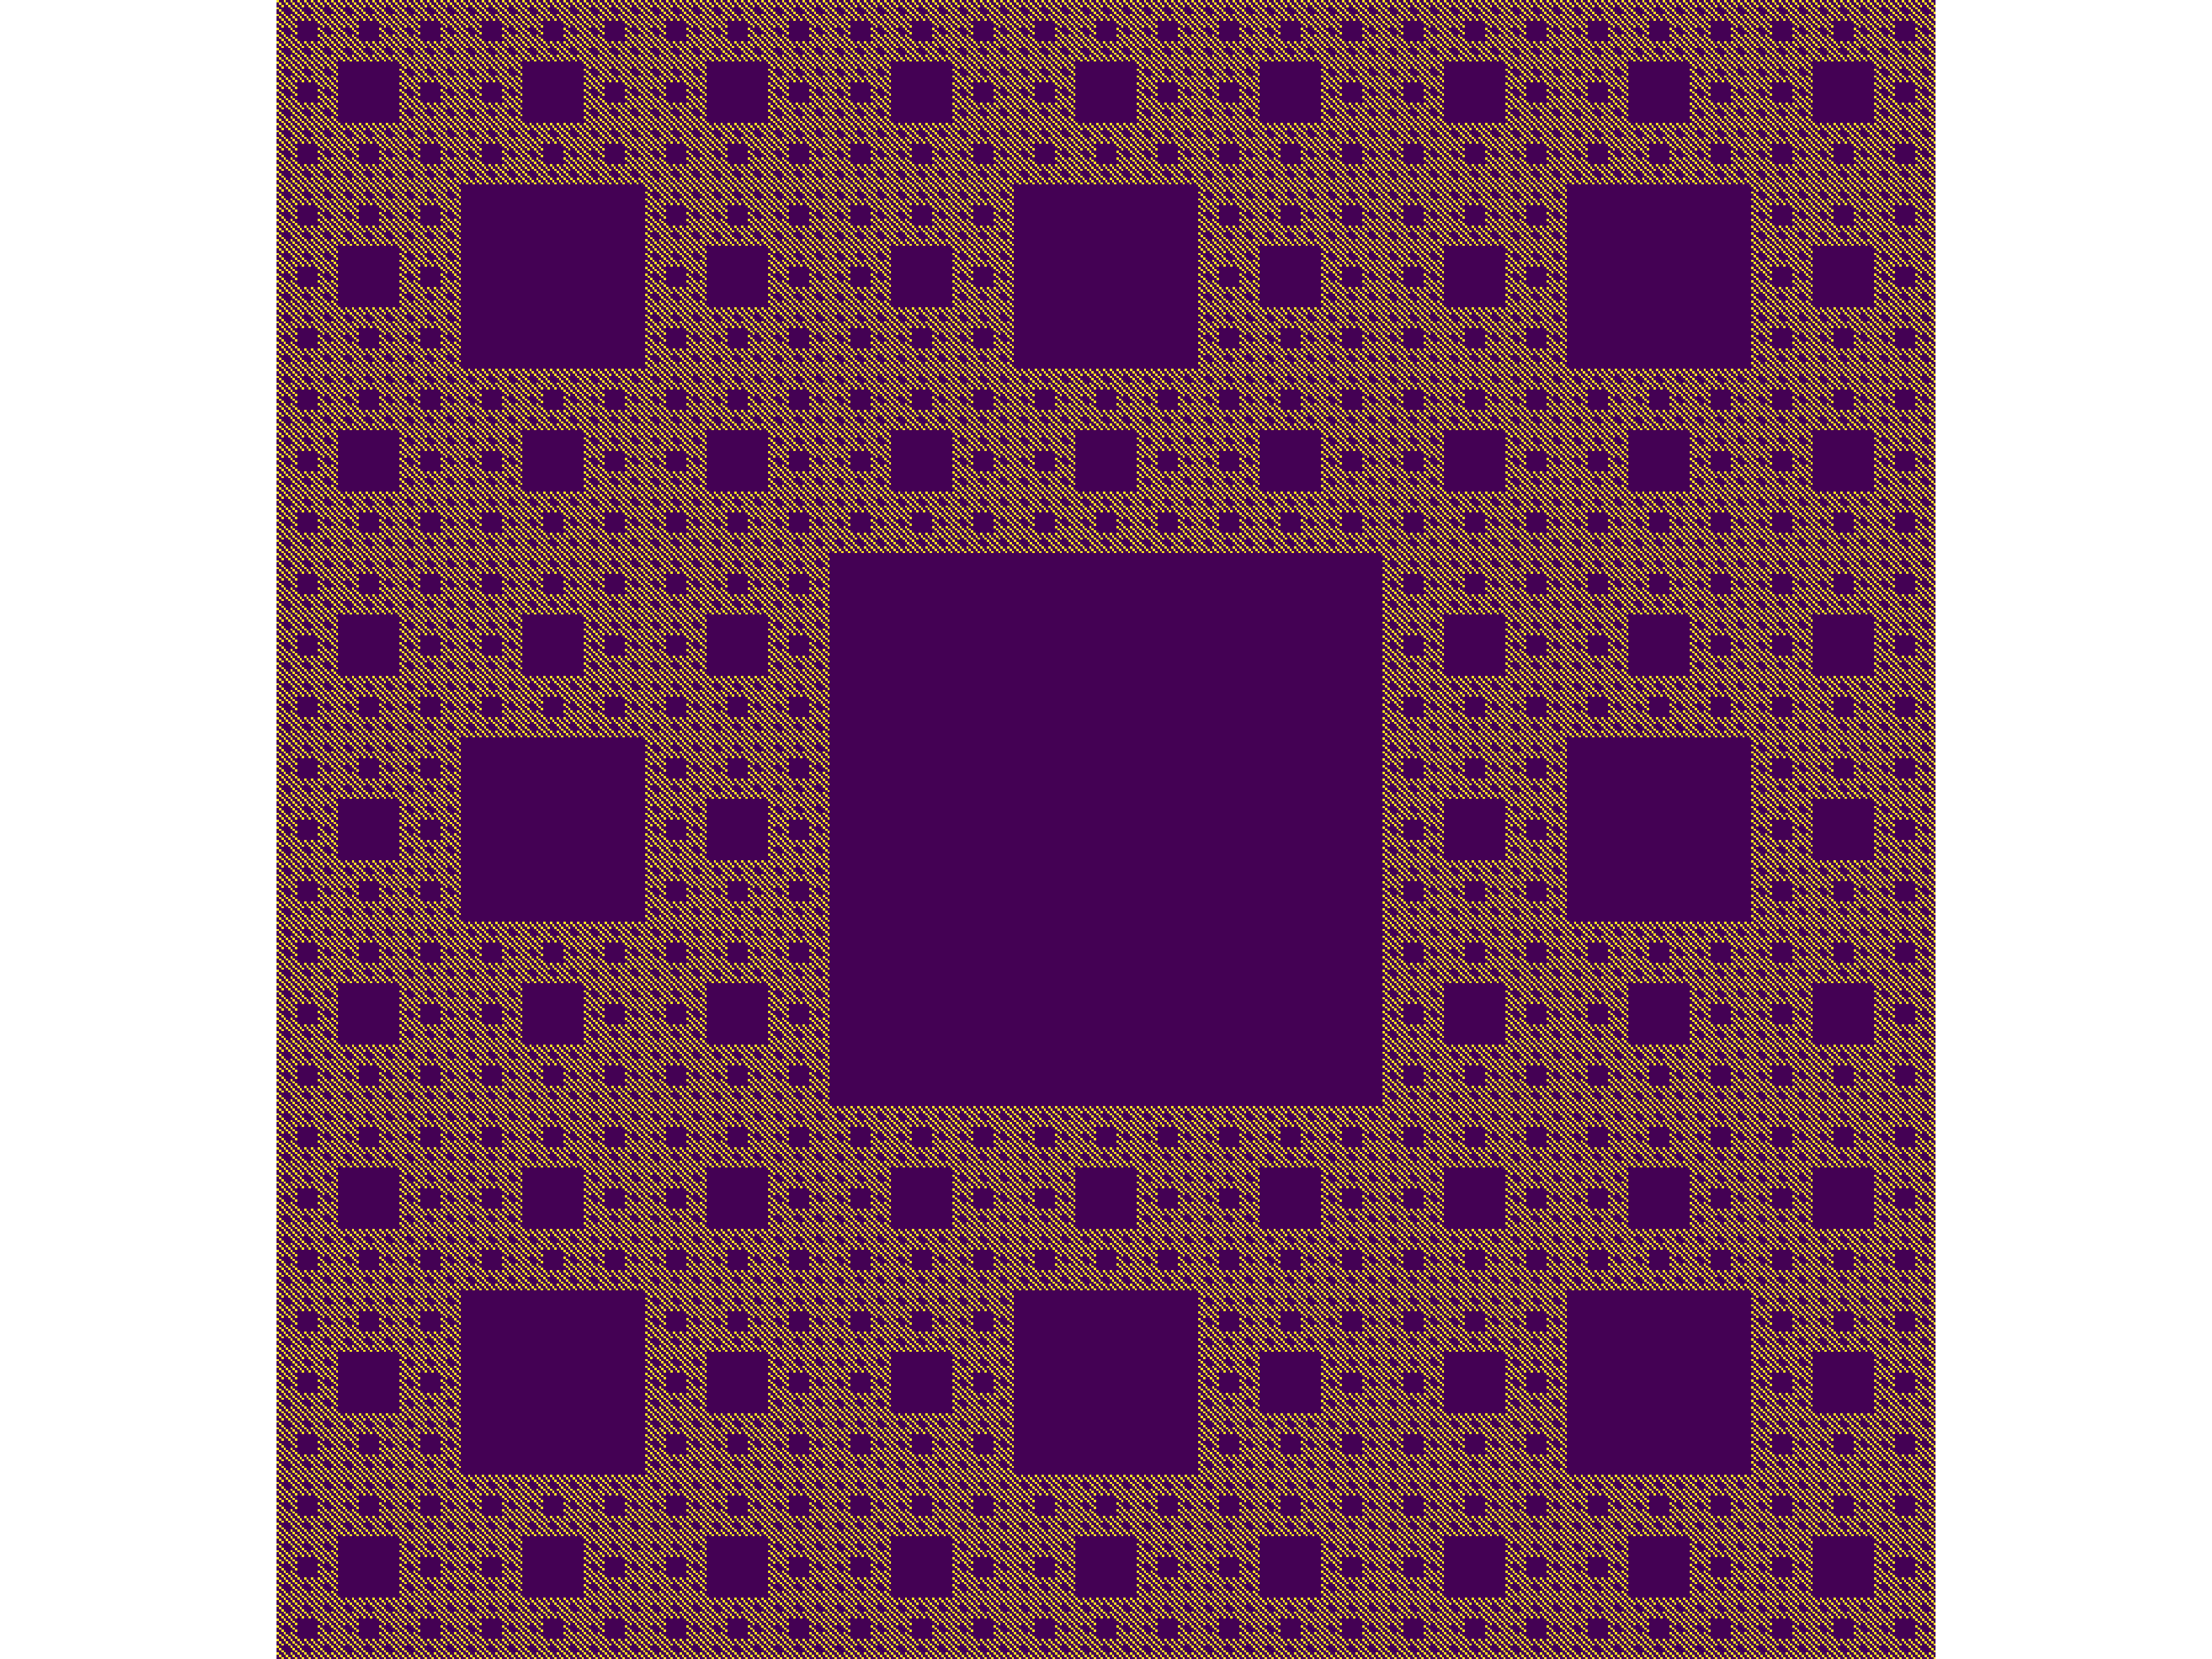
\includegraphics[width=0.38\textwidth]{media/sierpinsky_carpet.png}
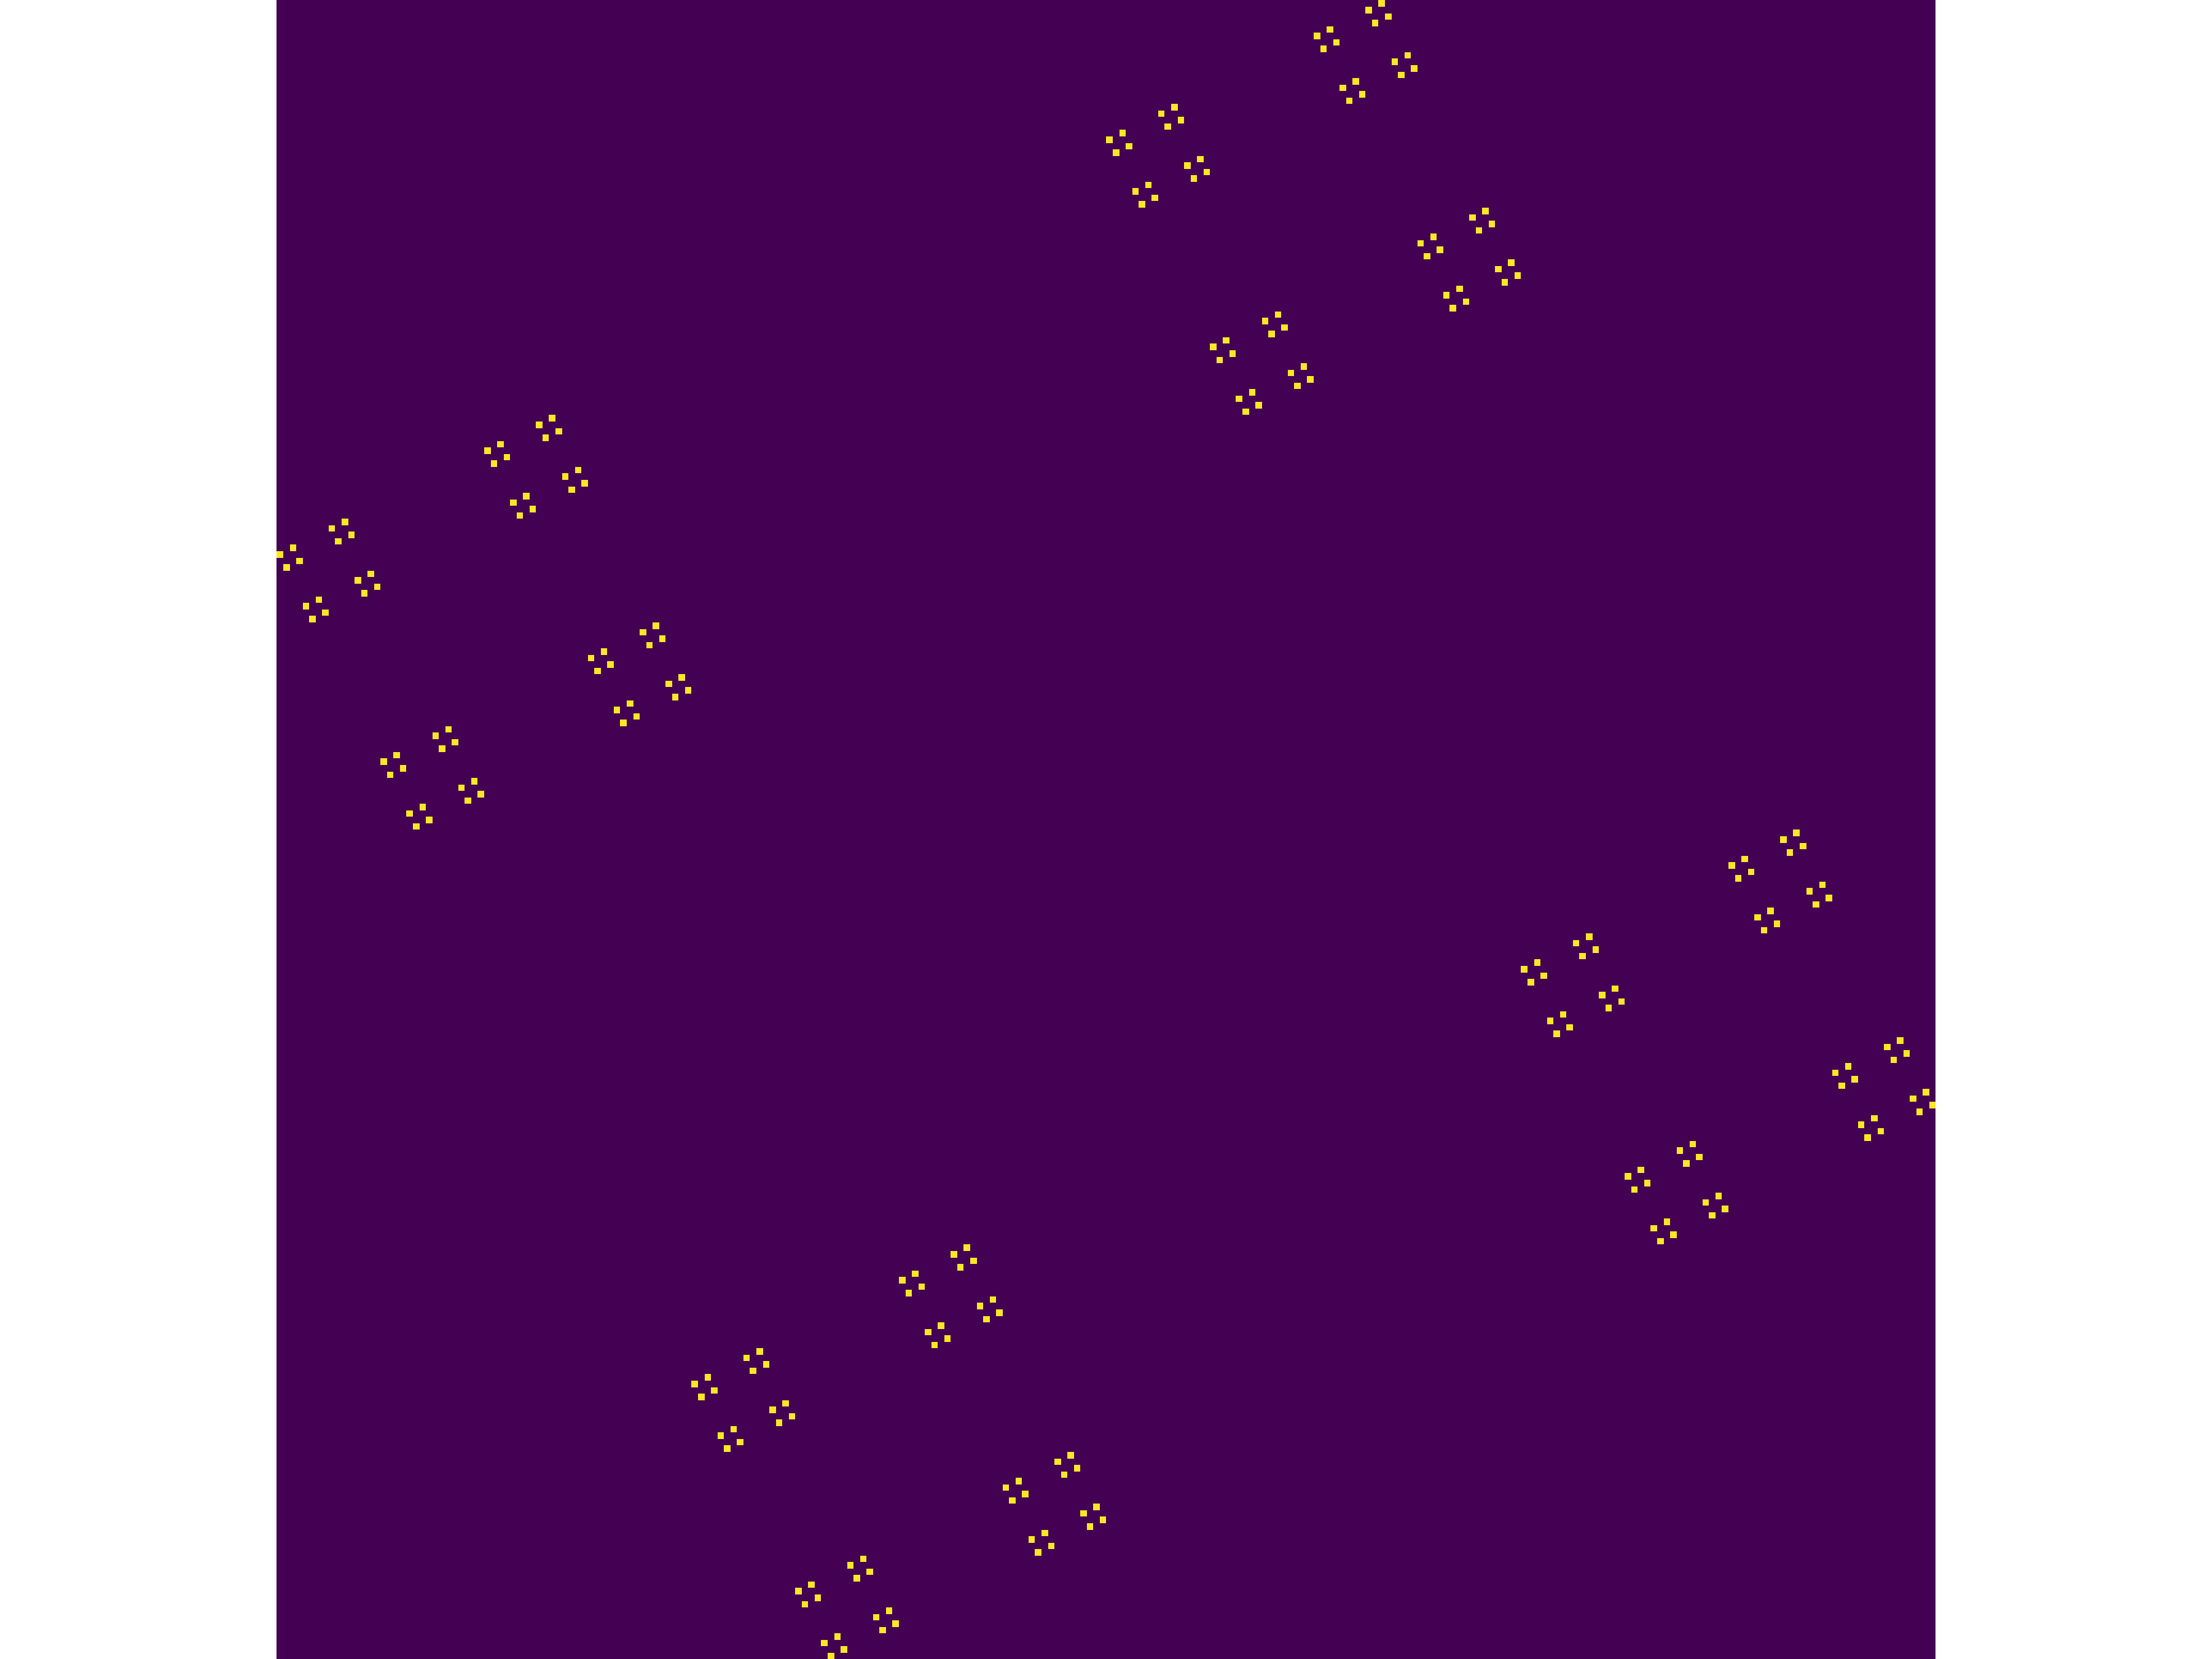
\includegraphics[width=0.38\textwidth]{media/Cantor_Dust_gen.png}
\end{center}



\paragraph{Sierpinski's Triangle}
\label{sec:org5c7c49d}
Not all fractal patterns can be produced by using recursive functions involving matrices, one such function is \emph{Sierpinski's Triangle}.
\subparagraph{Chaos Game}
\label{sec:org4d4956f}
The chaos game is a technique that can generate fractals, one of the advantages of this approach is that it can provide an estimate of the theoretical measure of a fractal without needing to iterate a function many times. The technique involves marking 3 points of an equilateral triangle and marking an arbitrary point, select one of these 3 points randomly with a uniform probability and create a new point halfway between the previous point and this point, repeat this process for as many points of detail are desired for the image.

This can be visualized by mapping the co-ordinates of an equilateral triangle to a Cartesian plane:

\begin{itemize}
\item \(A\)  \(\left(0, 0\right)\)
\item \(B\)  \(\left(0, 1\right)\)
\item \(C\)  \(\left(0.5, \sin\left(\frac{\pi}{3}\right)\right)\)
\end{itemize}

The mean value of the \(x\), \(y\) values for these co-ordinates is equal to the
halfway point and using this the chaos game can be implemented as a program and
visualized by plotting each point on a scatter plot. This is implemented in
\emph{\textbf{R}} in listing \ref{l-sier-tri} and the output is shown in Figure \ref{fig:s-tri}.

To measure the fractal dimension of this could be done by mapping the Cartesian
plane back to a matrix and taking the same approach as previous fractals
presented, this however was not implemented, due to time constraints, the
dimension was however measured using the method discussed at \S \ref{pas-tri}.

\newpage
\begin{listing}[htbp]
\begin{minted}[]{r}
library(ggplot2)
# Parameters
n <- 50000
df <- data.frame("xval"=1:n, "yval"=1:n)
# Constants
x <- c(runif(1), runif(1))
A <- c(0, 0)
B <- c(1, 0)
C <- c(0.5, sin(pi/3))
# Loop
for (i in 1:n) {
    dice = sample(1:3, 1)
    if (dice == 1) {
        x <- (x + A)/2
        df[i,] <- x
    } else if (dice == 2) {
        x <- (x + B)/2
        df[i,] <- x
    } else {
        x <- (x + C)/2
        df[i,] <- x
    }
}
# Plot
ggplot(df, aes(x = xval, y = yval)) +
    geom_point(size = 1, col = "cadet blue") +
    theme_classic()

\end{minted}
\caption{\label{l-sier-tri}R code to construct Sierpinksi's triangle through the Chaos Game, shown in Figure \ref{fig:s-tri}.}
\end{listing}

\newpage
\begin{wrapfigure}{l}{0.5\textwidth}
\centering
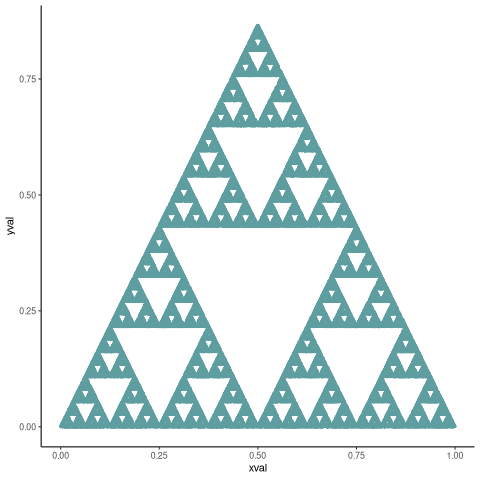
\includegraphics[width=0.38\textwidth]{pascal-sierpinsky-chaos-game.png}
\caption{\label{fig:s-tri}Sierpinski's Triangle created using the \emph{Chaos Game} in listing \ref{l-sier-tri}.}
\end{wrapfigure}

\subparagraph{Pascals Triangle\hfill{}\textsc{Ryan}}
\label{pas-tri}
The even and odd values in \emph{Pascal's Triangle} demonstrate the same pattern as
the \emph{Sierpinski Triangle} this is discussed in greater detail in \S
\ref{pascal-sierpinski}, implementing this to produce the sierpinski triangle is very
simple, it is however significantly more resource intensive, even in \emph{Julia}
than using the chaos game and the the measured dimension converges to the self
similar dimension very slowly.

The fractal produced is composed of right angle triangles, as opposed to equilateral triangles but interestingly the measured dimension is still the same as an equilateral \emph{Sierpinski's Triangle}, it does however converge to this value slowly.

\begin{listing}[htbp]
\begin{minted}[]{julia}
function pascal(n)
    mat = [isodd(binomial(BigInt(j+i),BigInt(i))) for i in 0:n, j in 0:n]
    return mat
end
GR.imshow(pascal(999))
GR.savefig("../../Report/media/pascal-sierpinsky-triangle.png")

#------------------------------------------------------------
#-- Calculate Dimension -------------------------------------
#------------------------------------------------------------

mat2 = pascal(300)
l2   = sum(mat2)
size2 = size(mat2)[1]
mat1 = pascal(200)
l1   = sum(mat1)
size1 = size(mat1)[1]
log(l2/l1)/log(size2/size1)
# https://en.wikipedia.org/wiki/Sierpi%C5%84ski_triangle
log(3)/log(2)

#------------------------------------------------------------
julia> log(l2/l1)/log(size2/size1)
1.8177195595512954
julia> log(3)/log(2)
1.5849625007211563


\end{minted}
\caption{\label{pascal-triangle-sierpinski}Julia code demonstrating Sierpinksi's triangle, this converges to the self similar dimension very slowly, using the ratio between a \(3000^{2}\) and \(2000^{2}\) matrix gave the correct answer to 2 decimal places, using a \(300^{2}\) and \(200^{2}\) matrix produced a value far of as shown.}
\end{listing}


\newpage
\subsubsection{Turtle\hfill{}\textsc{Ryan}}
\label{turtle}
\begin{wrapfigure}{r}{0.4\textwidth}
\centering
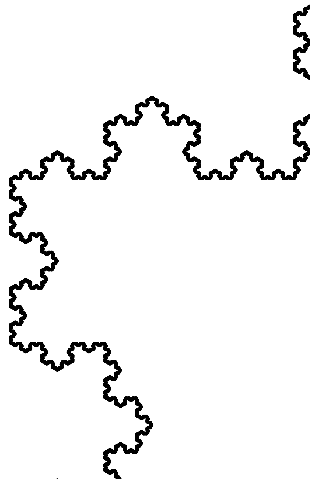
\includegraphics[width=0.25\textwidth]{../Problems/Chaos/Spirals/snowCurve.png}
\caption{\label{snow-turtle}Portion of the Koch Snowflake Produced by the Turtle graphics in listing \ref{turtle-snow}}
\end{wrapfigure}


Some Fractals cannot be well explained by using matrices or the chaos game, Turtle graphics are a programmatic way to draw a pen across a screen, these are implemented in \emph{Julia} using the \emph{Luxor} package \cite{JuliaGraphicsLuxorJl2020}.



We were unfourtunately unable to implement a strategy to measure the dimension
of such fractals, one such approach that looked promising but did not return
consistent results was to export the generated image to a PNG and then import
that file as a matrix using the \emph{Python Pillow Library} \cite{PillowPillowPIL} or
the \emph{Julia Images} library \cite{JuliaImagesImagesJl2020}, when this was
unsucessful we also experimented with \emph{ImageMagick} \cite{llcImageMagick},
\emph{AstroPy} \cite{Astropy} and \emph{JuliaAstro} \cite{JuliaAstroJuliaAstro}.
Unfourtunately the values returned by this approach were inconsistent and
further investigation into this method is required.


\begin{wrapfigure}{l}{0.3\textwidth}
\centering
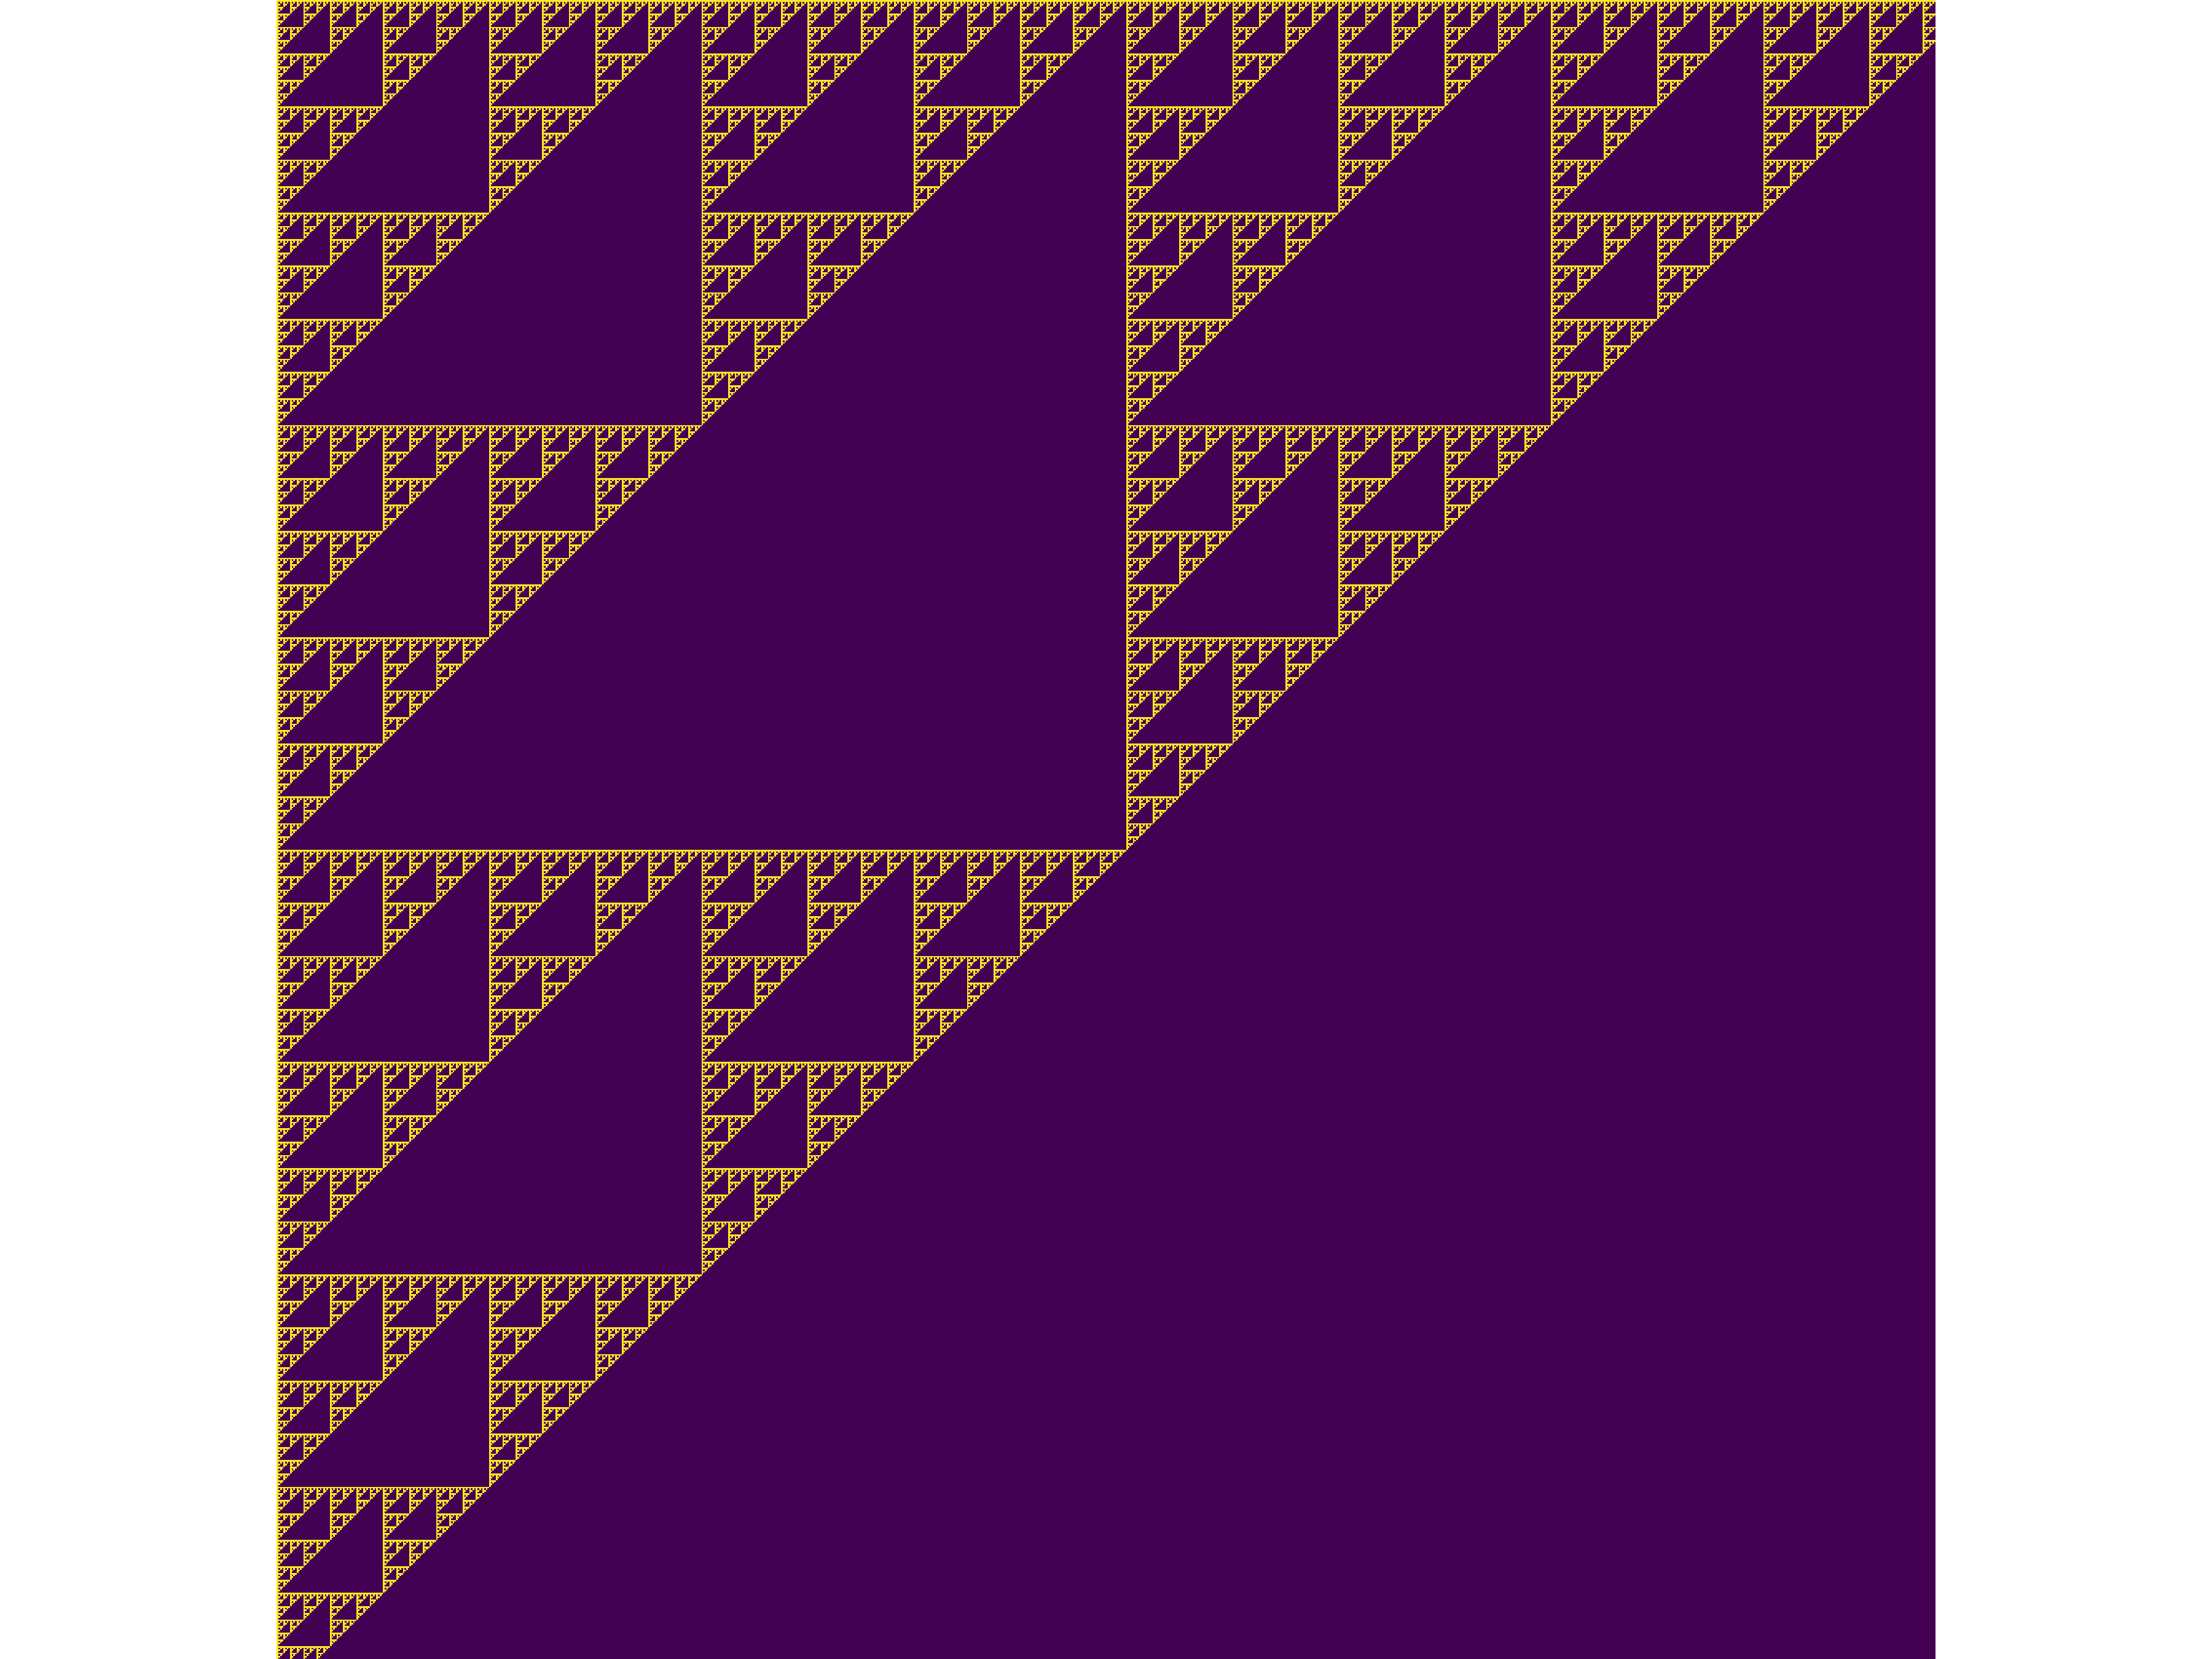
\includegraphics[width=0.25\textwidth]{media/pascal-sierpinsky-triangle.png}
\caption{\label{fig:pascal-sierpinsky}Sierpinski's triangle generated}
\end{wrapfigure}

The koch snowflake can be implemented by recursively calling a function that draws the first level of a koch curve, if this function decrements a provided level and is defined to call itself for each arm of the curve unless the level has reached zero it will produce a koch snowflake at the specified level, this is implemented in listing \ref{turtle-snow} and shown in Figure \ref{snow-turtle}.

\begin{listing}[htbp]
\begin{minted}[]{julia}
using Shapefile
using Luxor
using Pkg

#------------------------------------------------------------
#--- Round Snowflake Working ---------------------------------
#------------------------------------------------------------
function snowflake(length, level, ♘)
    if level == 0
        Forward(♘, length)
        Circle(♘, 1)
        return
    end
    length = length/9
    snowflake(length, level-1, ♘)
    Turn(♘, -60)
    snowflake(length, level-1, ♘)
    Turn(♘, 2*60)
    snowflake(length, level-1, ♘)
    Turn(♘, -60)
    snowflake(length, level-1, ♘)
end

♘ = Turtle()
@png begin
for i in 1:3
    levels = 9
    Pendown(♘)
    snowflake(8^(levels-1), levels, ♘)
    Turn(♘, 120)
end
end 600 600 "snowCurve.png"

\end{minted}
\caption{\label{turtle-snow}Generate a Koch Snowflake using a Turtle Diagram}
\end{listing}

The dragon curve is slightly more complicated and can be implemented by two separate functions, one to turn and trigger a motion and the other to control in which direction to turn, this is implemented in \emph{Julia} in listing \ref{turtle-dragon}  and shown in Figure .

\begin{listing}[htbp]
\begin{minted}[]{julia}
using Shapefile
using Luxor

#------------------------------------------------------------
#--- Dragon -------------------------------------------------
#------------------------------------------------------------
# Define the Parent Function
function dragon(♘, order, length)
    print(" ") # Don't remove this or code breaks, I don't know why?
    Turn(♘, order*45)
    dragon_iterate(♘, order, length, 1)
end
# Define the Helper Function
function dragon_iterate(♘, order, length, sign)
    if order==0
        Forward(♘, length)
    else
        rootHalf = sqrt(0.5)
        dragon_iterate(♘, order -1, length*rootHalf, 1)
        Turn(♘, sign * -90)
        dragon_iterate(♘, order -1, length*rootHalf, -1)
    end
end
# Draw the Image
@png begin
    ♘ = Turtle()
    # Start from left to centre result
    Turn(♘, 180)
    Penup(♘)
    Forward(♘, 200)
    Pendown(♘)
    Turn(♘, 180)
    # Create the Output
    dragon(♘, 15, 400)
end 1000 1000

# Create many images
;mkdir /tmp/dragon
for i in range(1, 15)
name = string("/tmp/dragon/d", lpad(d, 5, "0"), ".png")
    @png begin
        ♘ = Turtle()
        # Start from left to centre result
        Turn(♘, 180)
        Penup(♘)
        Forward(♘, 200)
        Pendown(♘)
        Turn(♘, 180)
        # Create the Output
        dragon(♘, 15, 400)
    end 1000 1000 name
end
montage -geometry 1000x1000 *.png dragon.png

\end{minted}
\caption{\label{turtle-dragon}\emph{Julia} code to produce the Dragon Curve shown in Figure \ref{fig:turtle-dragon}}
\end{listing}



\begin{figure}[htbp]
\centering
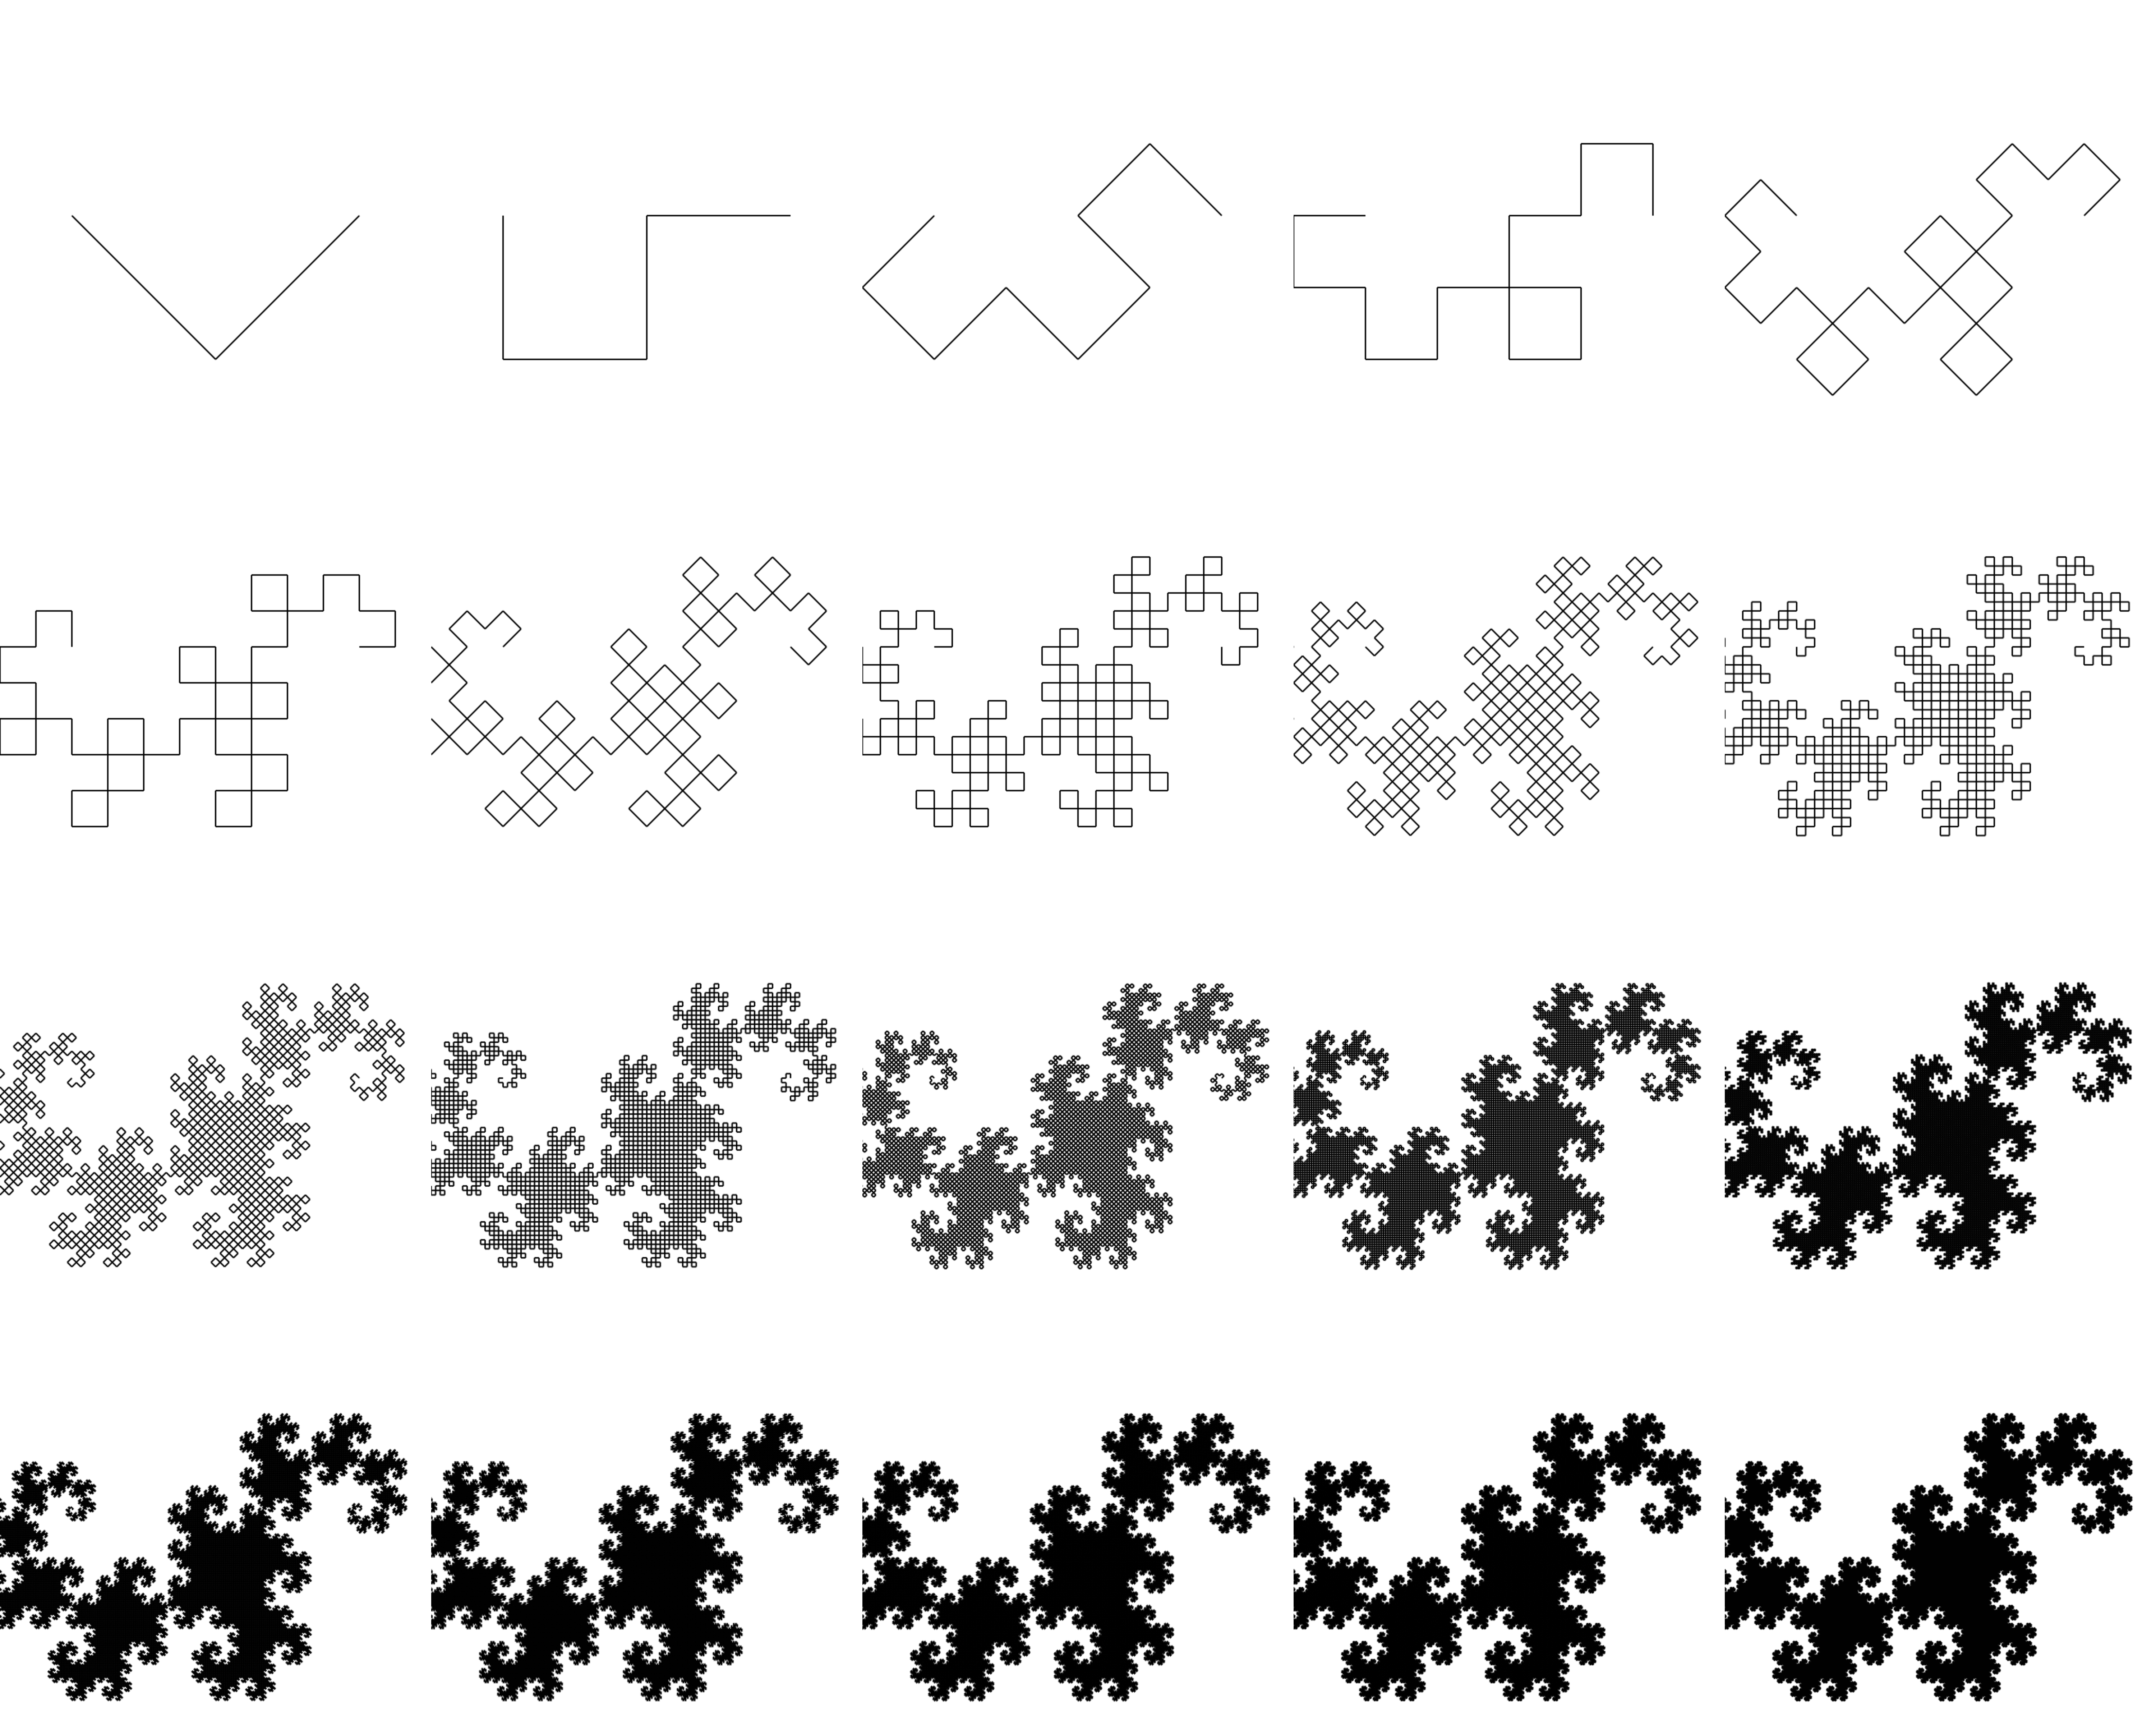
\includegraphics[width=9cm]{../Problems/Chaos/Spirals/dragon.png}
\caption{\label{fig:turtle-dragon}Progression of the Dragon Curve, this is known as a space filling curve \cite[p. 350]{peitgenChaosFractalsNew2004} which is a curve with a range that contains the entire 2-dimensional unit square \cite{ventrellaSpaceFillingCurvesAre2014}, it has a dimension of two. For some historical background on the curve on the origins of this curve see \cite{tabachnikovDragonCurvesRevisited2014}.}
\end{figure}




\subsubsection{Pascals Triangle and Sierpinski's Triangle\hfill{}\textsc{James}}
\label{pascal-sierpinski}
\paragraph{Motivation}
\label{sec:org784d58c}
Over many centuries, mathematicians have been able to produce a range of patterns from Pascal's triangle. One of which is relevant to the emergence of Sierpinski's triangle. To construct Pascal's triangle it begins with a 1 in the \(0^{th}\) (top) row, then each row underneath is made up of the sum of the numbers directly above it, see Figure \ref{fig:pascal-triangle}. Alternatively, the \(n^{th}\) row and \(k^{th}\) column can be written in combinatorics form, \(\binom{n}{k} = \binom{n-1}{k-1} + \binom{n-1}{k}\).

\begin{center}
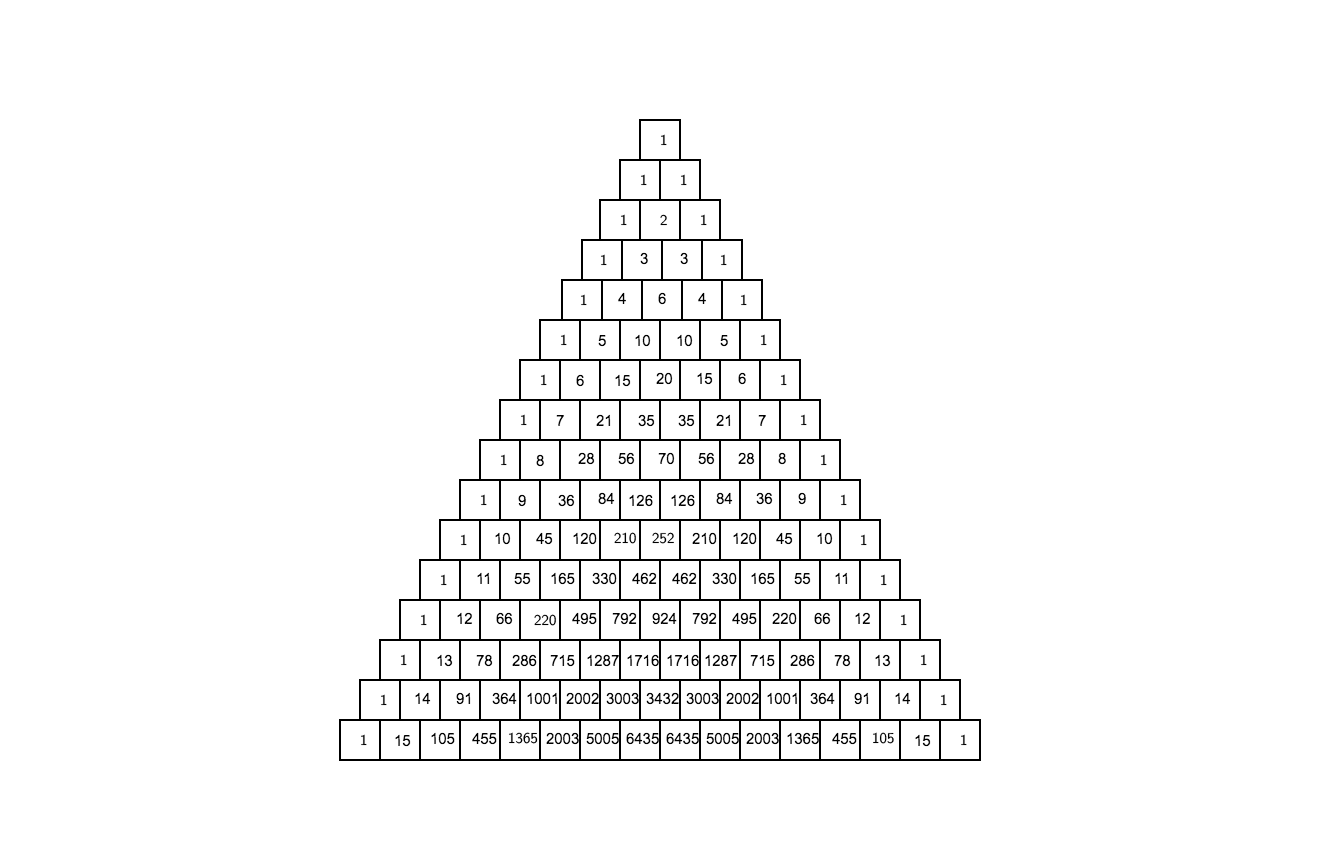
\includegraphics[width=.9\linewidth]{media/tikz/pascals-triangle.png}
\end{center}

\paragraph{The connection}
\label{sec:orga6f1a94}
As mentioned before there is one pattern that produces the Sierpinski triangle, namely highlighting all odd numbers in Pascal's triangle. This is equivalent to considering all the numbers in the triangle modulo 2, shown in Figure \ref{fig:pascal-sierpinski-tri}.

\begin{figure}[htbp]
\centering
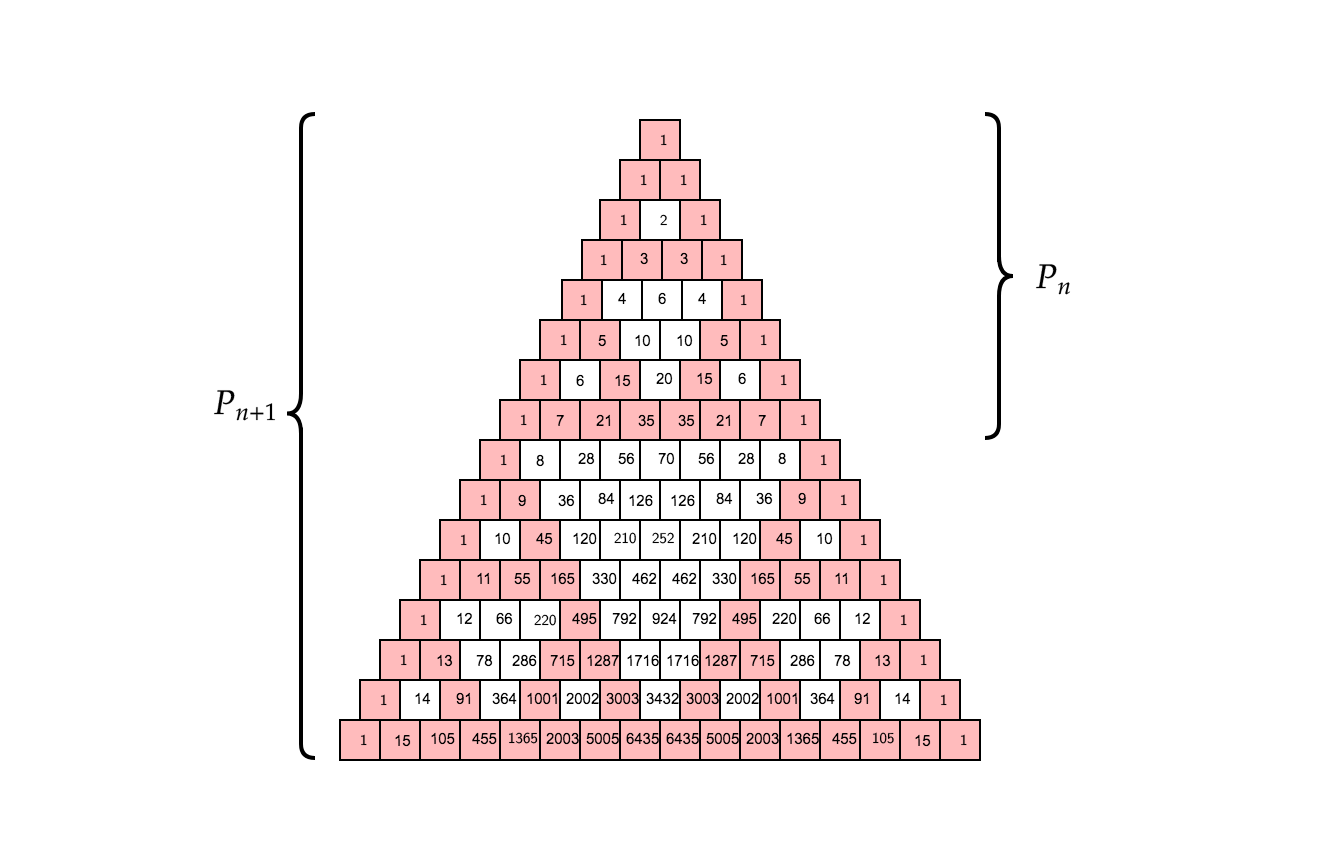
\includegraphics[width=9cm]{media/tikz/pascal-sierpinski-tri.png}
\caption{\label{fig:pascal-sierpinski-tri}Pascals Triangle coloured red for odd values}
\end{figure}

\begin{figure}[htbp]
\centering
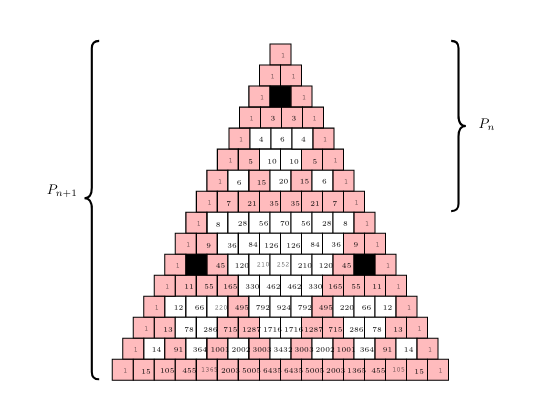
\includegraphics[width=9cm]{media/tikz/row-column-pascal.png}
\caption{\label{fig:row-column-pascal}The black squares represent one example of a position on Pascal's triangle that are equivalent modulo 2}
\end{figure}

In Figure \ref{fig:pascal-sierpinski-tri}, we can observe that all the highlighted odd numbers begin to form the Sierpinski triangle. Note that this is not the complete Sierpinski's triangle, that would require an infinite number of iterations. Now, we also notice that there are three identical Sierpinski triangles within the larger triangle, each containing the same value modulo 2, at each corresponding row and column.

To prove this, we need to split the triangle into two parts, \(P_{n}\) denoting the first \(2^{n}\) rows, i.e. the top ``Sierpinski triangle'' in Figure \ref{fig:pascal-sierpinski-tri} and \(P_{n+1}\) representing the entire triangle. We must show that any chosen square in \(P_{n}\) is equal to the corresponding row and column in the lower two triangles of \(P_{n+1}\), shown in Figure \ref{fig:row-column-pascal}. This requires an identity that allows us to work with combinations in modulo 2, namely Lucas' Theorem.

\paragraph{The connection}
\label{sec:org73b7ccb}
Let \(n,k \ge 0\) and for some prime \(p\), we get:
\begin{equation}
\binom{n}{k} = \prod_{i=0}^{m} \binom{n_i}{k_i} \quad (\text{mod}~p)
\end{equation}
where,
\begin{align*}
n &= n_{m}p^{m}+n_{m-1}p^{m-1}+\cdots + n_{1}p+n_{0},\\
k &= k_{m}p^{m}+k_{m-1}p^{m-1}+\cdots + k_{1}p+k_{0}\\
\end{align*}
are the expansions in radix \(p\) \footnote{Radix refers to a numerical system which uses some number of digits. Since we are working in modulo 2 for Pascal's triangle, we are only concerned with the numbers \(0\) or \(1\), i.e. a radix 2 or a binary numeric system.}. This uses the convention that \(\binom{n}{k} = 0\) if \(k < n\)

Take some arbitrary row \(r\) and column \(c\) in the triangle \(P_{n}\). If we add \(2^{n}\) rows to \(r\), we will reach the equivalent row and column in the lower left triangle of \(P_{n+1}\), since there are \(2^{n}\) rows in \(P_{n}\). In the same way, if we add \(2^{n}\) columns to \(c\) we reach the equivalent row and column in the lower right triangle of \(P_{n+1}\), leaving us with:

\begin{align*}
\text{Top Triangle:} \quad &\binom{r}{c}  \\
\text{Bottom-left Triangle:}\quad &\binom{r + 2^n}{c}  \\
\text{Bottom-right Triangle :}\quad &\binom{r + 2^n}{c + 2^n} \label{eq:bottom-right}
\end{align*}

Using Lucas' theorem, we can prove that the above statments are equivalent.

We can rewrite \(r\) and \(c\) in base 2 notation as follows:
\begin{align*}
r=r_{i}2^{i}+r_{i-1}2^{i-1}+\cdots + r_{1}2+r_{0}= \left[r_{i}r_{i-1}\cdots r_{1}r_{0}\right]_2\\
c=c_{i}2^{i}+c_{i-1}2^{i-1}+\cdots +c_{1}2+c_{0}=\left[c_{i}c_{i-1}\cdots c_{1}c_{0}\right]_2\\
\end{align*}

\begin{align*}
\binom{2^n + r}{c} &\equiv \binom{1r_{i-1}r_{i-2} \cdots r_{0}}{0c_{i-1}c_{i-2} \cdots c_{0}} \quad &(\text{mod} 2)\\
&\equiv \binom{1}{0}\binom{r_{i-1}}{c_{i-1}}\binom{r_{i-2}}{c_{i-2}} \cdots \binom{r_0}{c_0} \quad &(\text{mod} 2)\\
&\equiv\binom{r_{i-1}}{c_{i-1}}\binom{r_{i-2}}{c_{i-2}} \cdots \binom{r_0}{c_0} \quad &(\text{mod} 2)\\
&\equiv \binom{r}{c} \quad &(\text{mod} 2)
\end{align*}

\begin{align*}
\binom{2^n + r}{2^n + c} &\equiv \binom{1r_{i-1}r_{i-2} \cdots r_{0}}{1c_{i-1}c_{i-2} \cdots c_{0}} \quad &(\text{mod} 2)\\
&\equiv \binom{1}{1}\binom{r_{i-1}}{c_{i-1}}\binom{r_{i-2}}{c_{i-2}} \cdots \binom{r_0}{c_0} \quad &(\text{mod} 2)\\
&\equiv \binom{r_{i-1}}{c_{i-1}}\binom{r_{i-2}}{c_{i-2}} \cdots \binom{r_0}{c_0} \quad &(\text{mod} 2)\\
&\equiv \binom{r}{c} \quad &(\text{mod} 2)
\end{align*}

Thus, \(\binom{r}{c} = \binom{2^n + r}{c} = \binom{2^n + r}{2^n + c} \quad (\text{mod} 2)\), which concludes the proof

\subsection{Fractal Dimensions Sans Self Similarity\hfill{}\textsc{Ryan}}
\label{sans-self}
Not all fractals demonstrate obvious self-similarity, coastlines, as
discussed in \S \ref{definition}, are a common example but are not unique in this
regard, many natural phenomena such as the distribution of galaxies, shape of
clouds, outline of mountains and the the path of Brownian motion have a fractal structure
 \cite[Ch. 2]{gouyetPhysicsFractalStructures1996} that does not exhibit
obvious self-similarity.

In order to measure the dimension of such fractals the log transformed measure
and scale can be compared on a scatter plot in order to confirm that the
relationship is linear, if the relationship is linear the dimension is constant
and equal to the slope of the line, (see e.g. \cite[\S 4.2]{vicsekFractalGrowthPhenomena1992},
\cite{sandersonFractalsAreTypically2017} and \cite{mandelbrotHowLongCoast1967}).

This approach is implemented to measure the dimension of the \emph{Julia Set} in \S \ref{dim-julia}.


\newpage
\section{Connecting Fractals to Natural Processes\hfill{}\textsc{Ryan}}
\label{my-fractal}
In order to better understand the ways in which complex fractal patterns can
emerge from simple processes, a simple process that
leads to the emergence of such a pattern has been constructed, this is not a pattern that we have been able to find discussed in the literature but it does show simple connection between simple processes, patterns and the emergence of values such as golden ratio and the Fibonacci Sequence.

\subsection{Constructing a Simple Process}
\label{sec:org3d32bca}
Consider a fractal that begins simply with a square
 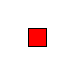
\begin{tikzpicture}\node at (3,0) [fill=red, rectangle,draw] (00) {};\end{tikzpicture} ,
imagine that this square is replicated, rotated and appended
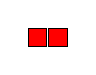
\begin{tikzpicture} \node[] (orig) at (0,0) {}; \node at (orig) [fill=red, rectangle,draw] {}; \node[xshift=1.72ex] at (orig) [fill=red, rectangle,draw] (01) {};\end{tikzpicture}
, then that shape, again is replicated rotated and appended
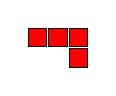
\begin{tikzpicture} \node[] (orig) at (0,0) {}; \node at (orig) [fill=red, rectangle,draw] {}; \node[xshift=1.72ex] at (orig) [fill=red, rectangle,draw] (01) {}; \node[xshift=3.44ex] at (orig) [fill=red, rectangle,draw] (01) {}; \node[xshift=3.44ex, yshift=-1.72ex] at (orig) [fill=red, rectangle,draw] (01) {}; \end{tikzpicture}
,this    process is illustrated in Figure \ref{My-Frac-progression-ink}, and if perpetuated a pattern emerges, as shown in Figure \ref{My-Frac-GR-plot}, this fractal can be generated by joining two matrices together in a manner that is consistent with the pattern described, this is shown in listing \ref{gen-frac-code}.

\begin{listing}[htbp]
\begin{minted}[]{julia}
function matJoin(A, B)
    function nrow(X)
        return size(X)[1]
    end
    function ncol(X)
        return size(X)[2]
    end
    emptymat = zeros(Bool, max(size(A)[1], size(B)[1]) ,sum(ncol(A) + ncol(B)) )
    emptymat[1:nrow(A), 1:ncol(A)] = A
    emptymat[1:nrow(B), (ncol(A)+1):ncol(emptymat)] = B
    return emptymat
end

function mywalk(B, n)
    for i in 1:n
        B = matJoin(B, rotl90(B));
    end
    return B
end

GR.imshow(mywalk([1, 1], 9))
\end{minted}
\caption{\label{gen-frac-code}Generate the fractal described in \S \ref{my-fractal} and shown in Figure \ref{My-Frac-GR-plot}}
\end{listing}



\begin{figure}[htbp]
\centering
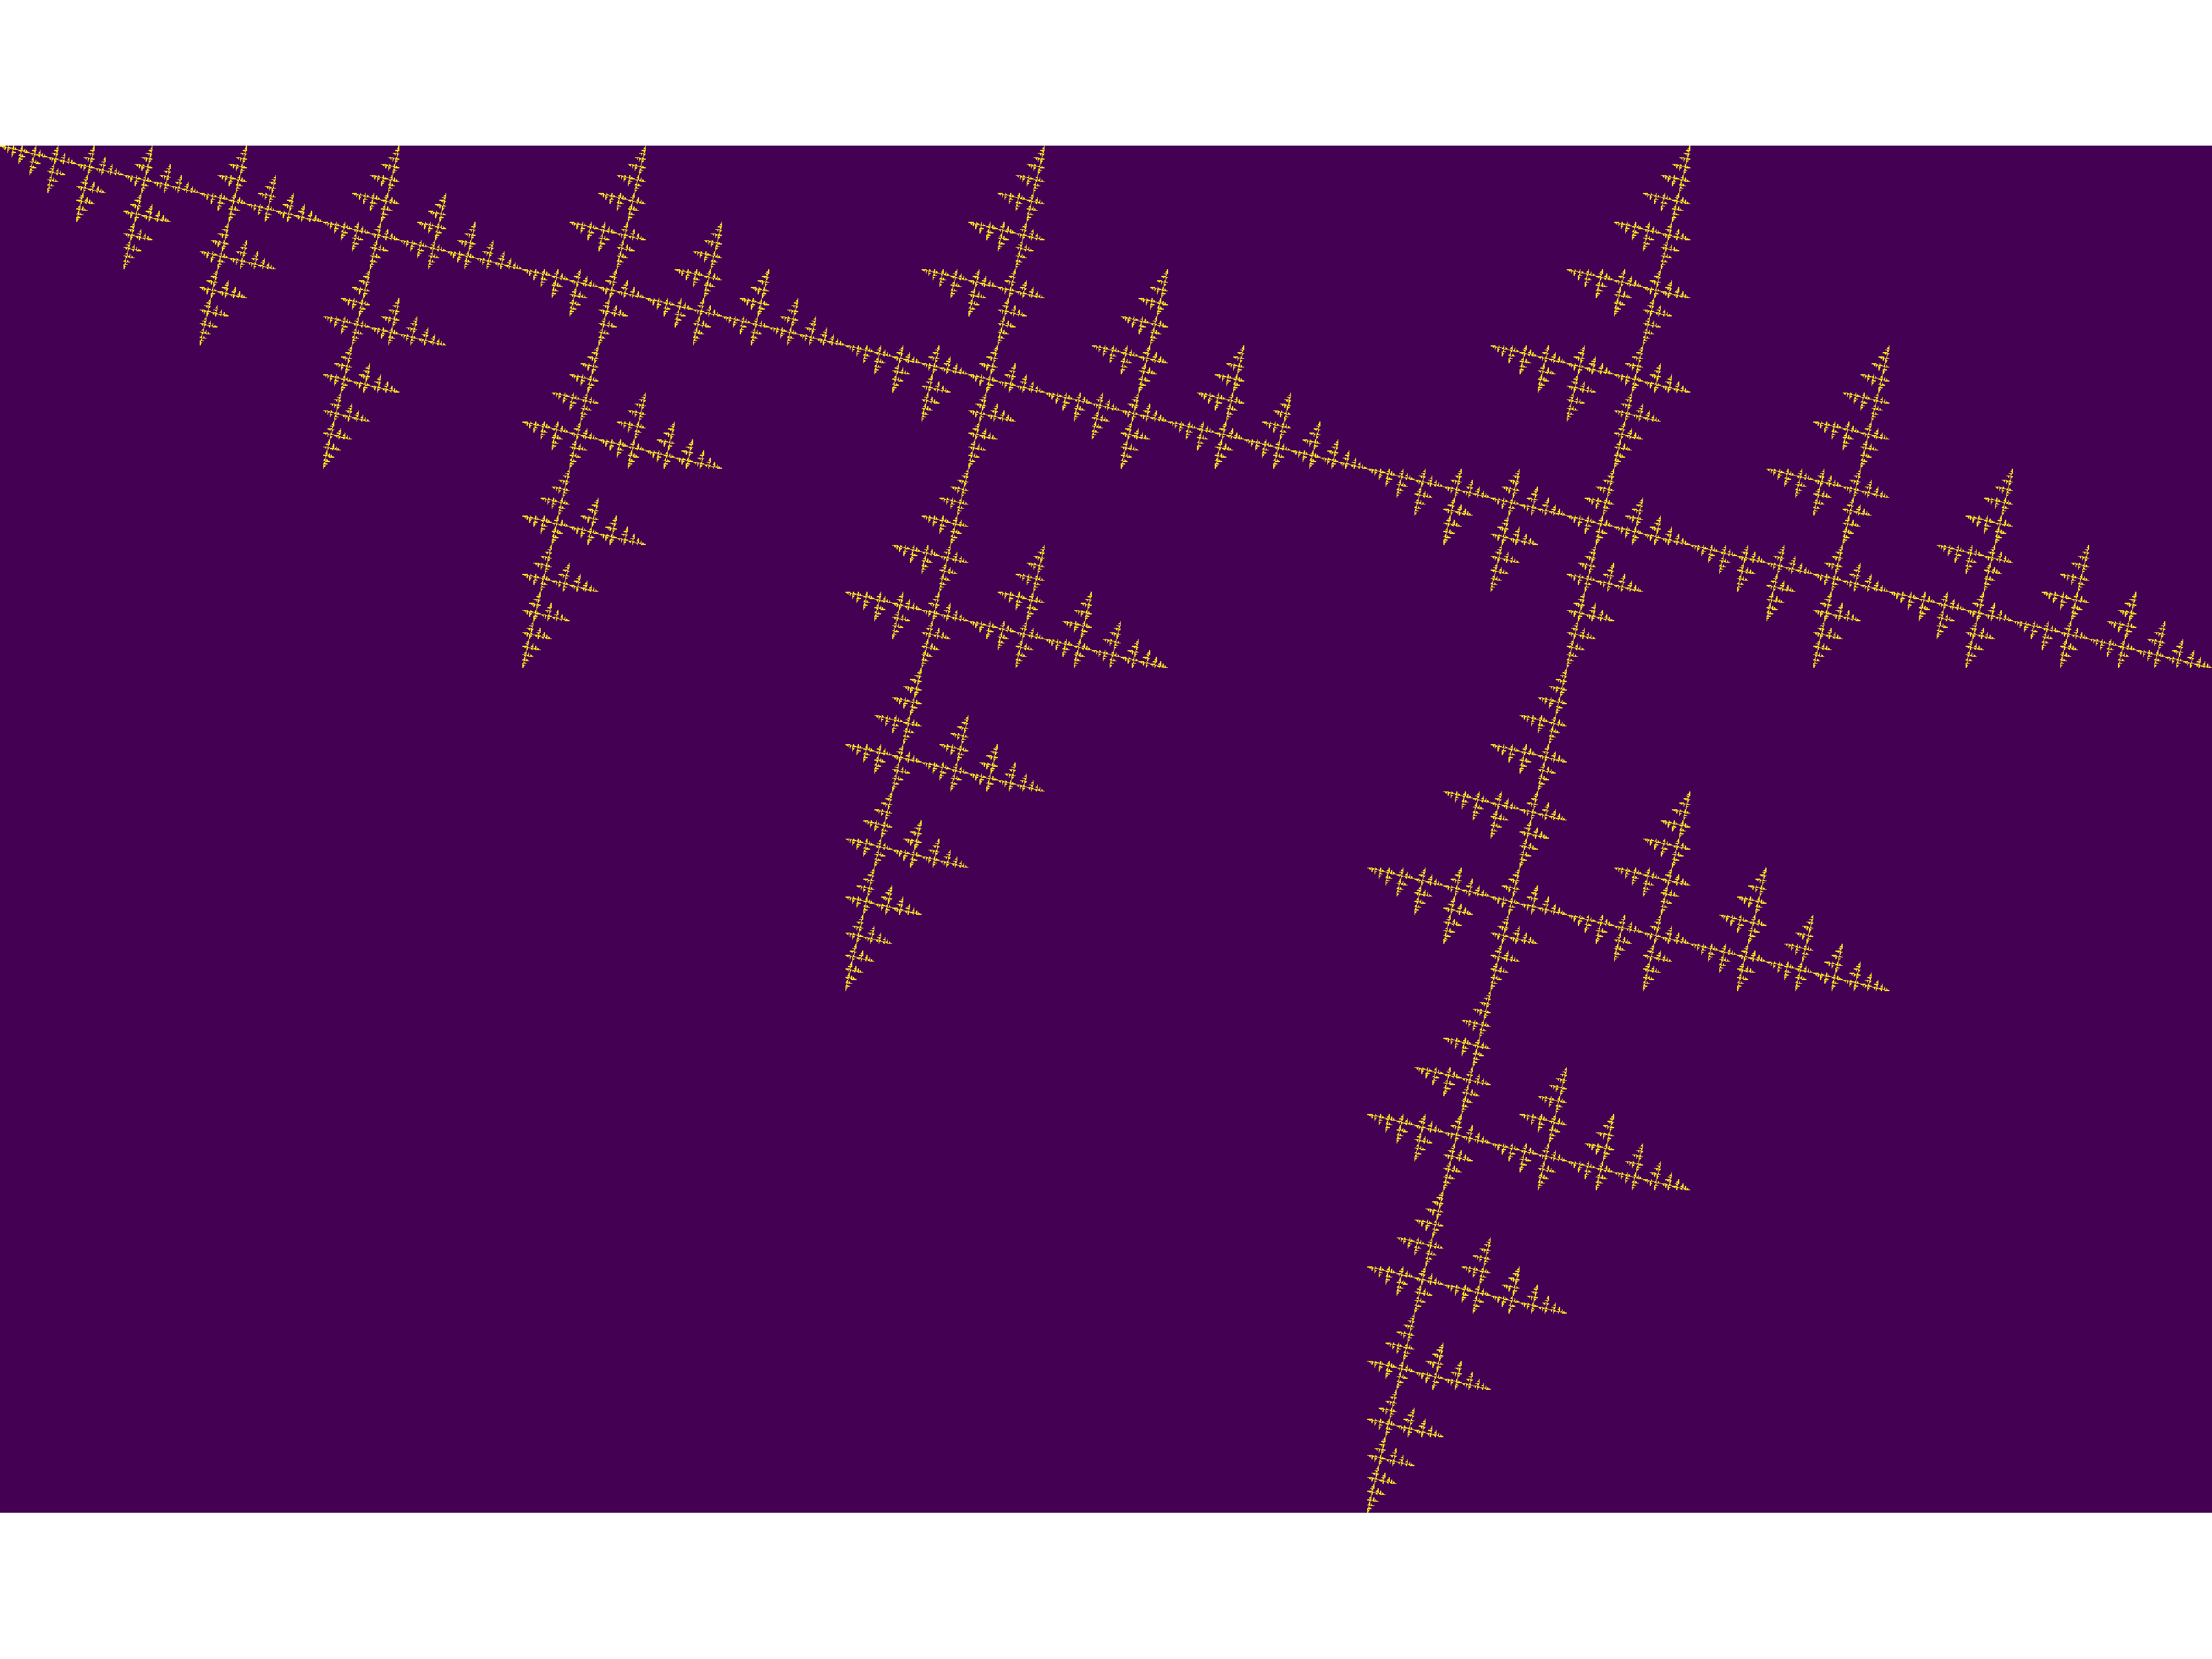
\includegraphics[width=.9\linewidth]{../Problems/fractal-dimensions/my-self-rep-frac-GR.png}
\caption{\label{My-Frac-GR-plot}Fractal that emerges by Rotating and appending boxes, this demonstrates the relationship between the Fibonacci numbers and golden ratio very well}
\end{figure}



\begin{figure}[htbp]
\centering
\includesvg[width=9cm]{../Problems/fractal-dimensions/My-Fib-Fractal-Diagram}
\caption{\label{My-Frac-progression-ink}Process to generate the fractal shown in Figure \ref{My-Frac-GR-plot} and described in \ref{My-Frac-ink-blue}. This process involves rotating and appending units and demonstrates a simple process from which the \emph{Fibonacci Numbers} emerge from simple processes.}
\end{figure}

\subsection{The Fibonacci Numbers}
\label{sec:org15913c4}

The fractal demonstrates a pattern that follows an angle that is caused by the
join of the replicated and rotated unit \footnote{The term unit is used because this pattern would emerge whether or not squares were used, squares are merely more convenient because they relate to the box-counting measure and may be easily visualised.}, the shape of these joins is a
rectangle that follows the Fibonacci numbers due to the additive nature of the
process, this is illustrated in Figure \ref{My-Frac-ink-blue}, in \S
it is shown that \(\lim
\left(\frac{F_{n}}{F_{n-1}}\right) = \varphi\), this means that the edges of the
fractal are proportional to one another as shown in listing \ref{My-Frac-ink-fade} and
so the angle can be given by the following relationship:

\begin{align}
    \theta &= \tan^{- 1} \left(\lim_{n \rightarrow \infty} \left(\frac{F_{n- 2}}{F_{n}}                 \right)        \right) \\
            &= \tan^{- 1} \left(\lim_{n \rightarrow \infty} \left(\frac{F_{n- 2}}{F_{n- 1}+  F_{n- 2}}   \right)        \right) \\
            &= \tan^{- 1} \left(\lim_{n \rightarrow \infty} \left(\frac{F_{n}}{F_{n+ 1}+  F_{n}}         \right)         \right)
	    \intertext{Because \(\lim_{n \rightarrow \infty} \left( \frac{F_n}{F_{n- 1}} \right) = \varphi \approx 1.618 \)  we can substite the values:} \notag\\
	    &= \tan^{-1} \left( \varphi\left( \varphi + 1  \right) \right) \\
	    &= \tan^{-1} \left( \frac{\psi}{\varphi +  1}\right) \\
	    &\approx 0.231^{\mathrm{c}}
\end{align}


this is illustrated in Figures \ref{My-Frac-ink-blue} and \ref{My-Frac-ink-fade}. This angle can be contrasted to the golden angle visualized in Figure \ref{My-Frac-gold-angle} and although different it interesting to note that \(2 \pi\left( \frac{\psi}{\varphi+1}\right) \equiv 2 \pi \psi \equiv 0 \pmod \psi\)
.


\begin{wrapfigure}{l}{0.5\textwidth}
\centering
\includesvg[width=0.25\textwidth]{../Problems/fractal-dimensions/golden-angle-diagram}
\caption{\label{My-Frac-gold-angle}Diagram of the Golden Angle, an angle formed by having a ratio of edges equal to the golden ratio.}
\end{wrapfigure}


\begin{figure}[htbp]
\centering
\includesvg[width=9cm]{../Problems/fractal-dimensions/my-self-rep-frac}
\caption{\label{My-Frac-ink-blue}TODO}
\end{figure}


\begin{figure}[htbp]
\centering
\includesvg[width=9cm]{../Problems/fractal-dimensions/scale-of-my-fractal}
\caption{\label{My-Frac-ink-fade}TODO}
\end{figure}

\subsection{The Dimension of the Fractal}
\label{sec:org286c021}
Each time this fractal is iterated the measure (i.e. the number of boxes) is doubled, but the scale of the fractal is increased by a ratio of the width and height, because the boxes add up this ratio will be a ratio of Fibonacci numbers which is shown to be equal to the golden ratio \(\phi\) in \S \ref{fib-golden-ratio-proof}, hence the dimension of this fractal is given by:

\begin{align}
\log_{\varphi}\left(2\right) &= \frac{\log (2)}{\log (\varphi)} \\
&\approx 1.44042
\end{align}

This value is consistent with measurements performed using \emph{Julia} in listing \ref{my-frac-measure-dim}.

\begin{listing}[htbp]
\begin{minted}[]{julia}
using DataFrames
function returnDim()
    mat2 = mywalk(fill(1, 1, 1), 10)
    l2   = sum(mat2)
    size2 = size(mat2)[1]
    mat1 = mywalk(fill(1, 1, 1), 11)
    l1   = sum(mat1)
    size1 = size(mat1)[1]
    df = DataFrame()
    df.measure = [log(l2/l1)/log(size2/size1)]
    df.actual  = [log(2)/log(1.618) ]
    return df
end

returnDim()

#------------------------------------------------------------
#  1×2 DataFrame
# │ Row │ measure │ actual  │
# │     │ Float64 │ Float64 │
# ├─────┼─────────┼─────────┤
# │ 1   │ 1.44052 │ 1.44048 │
\end{minted}
\caption{\label{my-frac-measure-dim}Measure the fractal dimension of the fractal described in \S \ref{my-fractal}}
\end{listing}

\section{The Fibonacci Sequence and the Golden Ratio}
\label{fib-golden-ratio-proof}
\subsection{The Golden Ratio\hfill{}\textsc{Ryan}}
\label{sec:org991cc2a}
The \emph{Fibonacci Sequence} and \emph{Golden Ratio} occur in many patterns observed
in natural phenomena (see
\cite{shellyallenFibonacciNature,benedettapalazzoNumbersNatureFibonacci2016,MinarovaNikoletta2014TFSN,NatureGoldenRatio2018,robertlambHowAreFibonacci2008,ronknottFibonacciNumbersGolden2016}),
an example of such an occurrence is discussed in section \ref{sunflower-example} and
a simple process demonstrating the emergence of the Fibonacci Numbers
is discussed in \S \ref{my-fractal}.

The Golden Ratio is a value \(\varphi\) that satisfies the following property:

\begin{align}
    \frac{a}{b} &=  \frac{a+  b}{a}= \varphi \nonumber \\
    \varphi &= 1+ \frac{1}{\varphi} \nonumber \\
    \implies  \varphi^2 &= \varphi +  1 \label{eq:phi-sim-to-fib-rec} \\
    \implies  \varphi &= \frac{1+ \sqrt{5} }{2} \label{eq:phi-value}
\end{align}

An interesting property of the golden ratio is that successive ratios of the
Fibonacci numbers converge to the golden ratio.

Consider the series:

$$\begin{aligned}
G_n &= \frac{F_{n} }{F_{n - 1} } \\
\end{aligned}$$

Such that \(F_{n}\) is the \(n^{\mathrm{th}}\) Fibonacci Number:

$$\begin{aligned}
F_n = F_{n- 1} +  F_{n- 2} ; \quad F_1 = F_2 = 1
\end{aligned}$$

\subsection{Golden Ratio In terms of the Fibonacci Sequence\hfill{}\textsc{James}}
\label{sec:org61af4d3}
The Series \(G\) is alternating convergent series, to show that consider the two sub-sequences formed by taking the odd and even ratios, these are both bounded monotone sequences.
\subsubsection{Prove that the Sequence is Bounded}
\label{sec:org6659f97}
Since we are trying to show that the ratio of Fibonacci numbers converges by the Monotone Convergence Theorem, we will let \(G_n\) be as follows:
\begin{equation*}
    G_n = \bigg\{ \frac{F_{n+1}}{F_n} \bigg\}_{n=1}^\infty, \quad F_1=F_2=1
\end{equation*}
To show \(G_n\) is bounded we must consider the following sub sequences,

\begin{enumerate}
\item \(\{G_{2n}\}_{n=1}^\infty\) is bounded below and decreasing
\item \(\{G_{2n-1}\}_{n=1}^\infty\) is bounded above and increasing
\end{enumerate}


Proving (i):\\

To show \(\{G_{2n}\}_{n=1}^\infty\) is decreasing we will show \(G_{2n} - G_{2(n+1)} > 0\) through the process of induction.

Proof: \\
For least element \(n = 1\):\\
\begin{align*}
    G_2 - G_4 &= \frac{F_3}{F_2} - \frac{F_5}{F_4}\\
    &= \frac{2}{1} - \frac{5}{3}\\
    &> 0
\end{align*}
Now assume true for all \(n\):\\
\begin{equation*}
    G_{2n} - G_{2(n+1)} > 0 \implies \frac{G_{2n}}{G_{2(n+1)}} > 1
\end{equation*}
Prove true for \(n+1\):
\begin{align*}
    G_{2(n+1)} - G_{2(n+2)} &= G_{2n + 2} - G_{2n+4)}\\
    &= \frac{F_{2n+3}}{F_{2n+2}} - \frac{F_{2n+5}}{F_{2n+4}}\\
    &= \frac{F_{2n+3}F_{2n+4} - F_{2n+5}F_{2n+2}}{F_{2n+2}F_{2n+4}}\\
    &= \frac{F_{2n+3}(F_{2n+3}+F_{2n+2}) - F_{2n+2}(F_{2n+4}+F_{2n+3})}{F_{2n+2}F_{2n+4}}\\
    &= \frac{(F_{2n+3})^2 - F_{2n+2}F_{2n+4}}{F_{2n+2}F_{2n+4}}\\
    &= \frac{(F_{2n+3})^2}{F_{2n+2}F_{2n+4}} - 1\\
    &= \frac{F_{2n+3}}{F_{2n+2}} \cdot \frac{F_{2n+3}}{F_{2n+4}} -1\\
    &= \frac{G_{2n+2}}{G_{2n+3}} - 1\\
\end{align*}
Since \(\frac{G_{2n}}{G_{2(n+1)}} > 1\) for all \(n\) by assumption, then \(\frac{G_{2n+2}}{G_{2n+3}} > 1\)  follows, hence
\begin{align*}
    G_{2(n+1)} - G_{2(n+2)} &= \frac{G_{2n+2}}{G_{2n+3}} - 1\\
    &> 1 -1\\
    &> 0
\end{align*}
Therefore by mathematical induction, \(G_{2n}\) is monotic decreasing.\\
Now, for \(\{G_{2n}\}_{n=1}^\infty\) to be bounded below we will consider the entire set \(G_n\), hence:
\begin{equation*}
    G_n = \frac{F_{n+1}}{F_n} =  \frac{F_n + F_{n-1}}{F_n} = 1 + \frac{F_{n-1}}{F_n}
\end{equation*}
Since all Fibonacci numbers are positive, \(\frac{F_{n-1}}{F_n} > 0\), so
\begin{equation*}
    G_n = 1 + \frac{F_{n-1}}{F_n} > 1
\end{equation*}
Thus \(G_n\) being bounded below implies \(G_{2n}\) is also bounded below.

Proving (ii):\\
To show \(\{G_{2n}\}_{n=1}^\infty\) is decreasing we will show \(G_{2n-1} - G_{2(n+1)-1} < 0\) through the process of induction.

Proof: \\
For least element \(n = 1\):\\
\begin{align*}
    G_1 - G_3 &= \frac{F_2}{F_1} - \frac{F_4}{F_3}\\
    &= \frac{1}{1} - \frac{3}{2}\\
    &< 0
\end{align*}
Now assume true for all \(n\):\\
\begin{equation*}
    G_{2n-1} - G_{2n+1} < 0 \implies \frac{G_{2n-1}}{G_{2n+1}} < 1
\end{equation*}
Prove true for \(n+1\):
\begin{align*}
    G_{2(n+1) -1} - G_{2(n+1) + 1} &= G_{2n+1} - G_{2n+3}\\
    &= \frac{F_{2n+2}}{F_{2n+1}} - \frac{F_{2n+4}}{F_{2n+3}}\\
    &= \frac{F_{2n+2}F_{2n+3} - F_{2n+4}F_{2n+1}}{F_{2n+1}F_{2n+3}}\\
    &= \frac{F_{2n+2}(F_{2n+2}+F_{2n+1}) - F_{2n+1}(F_{2n+3}+F_{2n+2})}{F_{2n+1}F_{2n+3}}\\
    &= \frac{(F_{2n+2})^2 - F_{2n+1}F_{2n+3}}{F_{2n+1}F_{2n+3}}\\
    &= \frac{(F_{2n+2})^2}{F_{2n+1}F_{2n+3}} - 1\\
    &= \frac{F_{2n+2}}{F_{2n+1}} \cdot \frac{F_{2n+2}}{F_{2n+3}} -1\\
    &= \frac{G_{2n+1}}{G_{2n+2}} - 1\\
\end{align*}
Since \(\frac{G_{2n-1}}{G_{2n+1}} < 1\) for all \(n\) by assumption, then \(\frac{G_{2n+1}}{G_{2n+2}} < 1\)  follows, hence
\begin{align*}
    G_{2(n+1)-1} - G_{2(n+1)+1} &= \frac{G_{2n+1}}{G_{2n+2}} - 1\\
    &< 1 -1\\
    &< 0
\end{align*}
Therefore by mathematical induction, \(G_{2n-1}\) is increasing.\\
Now, for \(\{G_{2n-1}\}_{n=1}^\infty\) to be bounded above we will again consider the entire set \(G_n\), hence:
\begin{equation*}
    G_n = \frac{F_{n+1}}{F_n} =  \frac{F_n + F_{n-1}}{F_n} = 1 + \frac{F_{n-1}}{F_n}
\end{equation*}
Since \(\frac{F_{n-1}}{F_n} \le 1\) we can deduce that
\begin{equation*}
    G_n = 1 + \frac{F_{n-1}}{F_n} \le 2
\end{equation*}
Thus \(G_n\) being bounded above by 2 implies \(G_{2n-1}\) is also bounded above by 2.
\subsubsection{Find the Limit}
\label{sec:org5dc73a6}
By the Monotone Convergence Theorem, \(\lim_{n \to \infty} G_n\) exists.
We will assume that \(G_{2n}\) and \(G_{2n-1}\) approach the same limit \(L~~\forall n \ge 1\)
Meaning, we will also take:

\begin{equation*}
    \lim_{n\to \infty}G_n = \lim_{n\to \infty}G_{n-1} = L
\end{equation*}

\begin{align*}
\lim_{n\to \infty}G_n &= \lim_{n \to \infty} \frac{F_{n} +  F_{n+  1} }{F_{n+  1} } \\
&= 1 +  \lim_{n \to \infty} \frac{F_{n- 1} }{F_n} \\
&=  1 +  \lim_{n \to \infty}\frac{1}{G_{n-1}} \\
 \implies L &= 1 + \frac{1}{L}\\
 L^2 &= L + 1\\
 0 &= L^2 - L - 1\\
  \implies  L &= \frac{\sqrt{5} + 1  }{2} = \varphi
\end{align*}
\subsection{Comments\hfill{}\textsc{Ryan}}
\label{comment}
In the 13\textsuperscript{th} century \footnote{Although scrictly speaking this sequence can be traced back to 200 BC \cite{prasadHowFibonacciNumber2018,brownHistoryApplicationsFibonacci2019}} Fibonacci developed \footnote{Or is it discovered?}  his namesake sequence when working on a problem concerning the growth rate
of a rabbit population \cite{ronknottFibonacciNumbersGolden2016}.
Continuous population growth is typically modelled with calculus by the equation \(\frac{\mathrm{d} }{\mathrm{d} t}\left( p \right)
\propto p\) \cite[\S 11.1]{giordanoFirstCourseMathematical2014}, what's interesting is that this population model itself
generates a fractal when the number of stationary points is plotted against the
growth rate \cite[Ch. 3]{briggsTurbulentMirrorIllustrated1989}
and this fractal is equivilant to a plot of the Mandelbrot Set (discussed in \S \ref{mandlebrot-set}) where the \(x\)-axis represents the real component of a value and the \(y\)-axis the number of iterations before a value exceeds a modulus of 2 (see generally \cite{mullerThisEquationWill2020}). This is not
something we had time to investigate unfourtunately but it does demonstrate the deep connection between natural phenomena such as population growth, the Fibonacci Sequence and complex fractals such as the Mandelbrot set.
\subsubsection{Equivalent forms of the Golden Ratio}
\label{sec:org6f71698}
The golden ratio is sometimes expressed in odd forms in the literature:


$$\begin{aligned}
\lim_{n     \rightarrow \infty }\left[ \frac{F_n}{F_{n- 1} }  \right] &= \varphi \\
\lim_{n     \rightarrow \infty }\left[ \frac{F_n}{F_{n- 1} }  \right] &= \psi \\
\varphi - \psi &=  1 \\
\varphi \times  \psi  &= 1 \\
\frac{\psi}{\varphi}  = \frac{1}{\varphi^2} = \frac{1}{1-\varphi} &= \frac{1}{2-\varphi} = \frac{2}{3 - \sqrt{5}  }
\end{aligned}$$
\subsection{A closed Solution for the Fibonacci Numbers\hfill{}\textsc{Ryan}}
\label{solving-the-sequence}
The Fibonacci numbers can be solved  using Calculus and this closed solution can be used to show that the ratio of Fibonacci numbers converges to the golden ratio. \footnote{For further material related to exponential generating function see \ref{exp-gen-func-fib-seq} of the appendix.}

Consider the \emph{Fibonacci Sequence}:


\begin{align}
    a_{n}&= a_{n - 1} + a_{n - 2} \nonumber \\
\iff a_{n+  2} &= a_{n+  1} +  a_n \label{eq:fib-def-shift}
\end{align}

From observation, this appears similar in structure to the following \emph{ordinary
differential equation}, which would be fairly easy to deal with:


\begin{align*}
f''\left( x \right)- f'\left( x \right)- f\left( x \right)=  0
\end{align*}

By ODE Theory we have \(y \propto e^{m_{i}x}, \enspace i = 1, 2\) \cite[\S 4.1.2]{zillDifferentialEquationsBoundaryvalue2009}
and the following power series \cite[\S 64]{churchillComplexVariablesApplications2014}:

\begin{align*}
f\left( x \right)= e^{mx} = \sum^{\infty}_{n= 0}   \left[ r^{m} \frac{x^n}{n!} \right]
\end{align*}

So using some sort of a transformation involving a power series may help to
relate the discrete problem back to a continuous one.

Consider using the following generating function, (proof of the
generating function derivative as in \eqref{eq:exp-gen-def-2} and \eqref{eq:exp-gen-def-3} is
provided in section \ref{Derivative-exp-gen-function})




\begin{align}
    f\left( x \right) &=  \sum^{\infty}_{n= 0}   \left[ a_{n} \cdot  \frac{x^n}{n!} \right]   \label{eq:exp-gen-def-1} \\
 \implies   f'\left( x \right) &=  \sum^{\infty}_{n= 0}   \left[ a_{n+1} \cdot  \frac{x^n}{n!} \right]   \label{eq:exp-gen-def-2} \\
\implies    f''\left( x \right) &=  \sum^{\infty}_{n= 0}   \left[ a_{n+2} \cdot  \frac{x^n}{n!} \right]   \label{eq:exp-gen-def-3}
\end{align}


So the Fibonacci recursive relation from \eqref{eq:fib-def-shift}  could be expressed :


\begin{align*}
a_{n+  2}    &= a_{n+  1} +  a_{n}\\
\frac{x^n}{n!}   a_{n+  2}    &= \frac{x^n}{n!}\left( a_{n+  1} +  a_{n}  \right)\\
\sum^{\infty}_{n= 0} \left[ \frac{x^n}{n!}   a_{n+  2} \right]        &= \sum^{\infty}_{n= 0}   \left[ \frac{x^n}{n!} a_{n+  1} \right]  + \sum^{\infty}_{n= 0}   \left[ \frac{x^n}{n!} a_{n}  \right]  \\
\end{align*}

And hence by applying \eqref{eq:exp-gen-def-1}, \eqref{eq:exp-gen-def-2} and \eqref{eq:exp-gen-def-3}:

\begin{align}
f''\left( x \right) &= f'\left( x \right)+  f\left( x \right)
\end{align}


Using the theory of higher order linear differential equations with
constant coefficients it can be shown:


\begin{align*}
f\left( x \right)= c_1 \cdot  \mathrm{exp}\left[ \left( \frac{1- \sqrt{5} }{2} \right)x \right] +  c_2 \cdot  \mathrm{exp}\left[ \left( \frac{1 +  \sqrt{5} }{2} \right)x \right]
\end{align*}


By equating this to the power series:


\begin{align*}
f\left( x \right)&= \sum^{\infty}_{n= 0}   \left[ \left( c_1\left( \frac{1- \sqrt{5} }{2} \right)^n +  c_2  \left( \frac{1+ \sqrt{5} }{2} \right)^n \right) \cdot  \frac{x^n}{n!} \right]
\end{align*}


Now given that:


\begin{align*}
f\left( x \right)= \sum^{\infty}_{n= 0}   \left[ a_n \frac{x^n}{n!} \right]
\end{align*}


We can conclude that:


\begin{align*}
a_n = c_1\cdot  \left( \frac{1- \sqrt{5} }{2} \right)^n +  c_2 \cdot  \left( \frac{1+  \sqrt{5} }{2} \right)^n
\end{align*}


By applying the initial conditions:


\begin{align*}
a_0= c_1 +  c_2  \implies  c_1= - c_2\\
a_1= c_1 \left( \frac{1+ \sqrt{5} }{2} \right) -  c_1 \left( \frac{1-\sqrt{5} }{2} \right)  \implies  c_1 = \frac{1}{\sqrt{5} }\\
\ \\
\therefore ~ c_1 = \frac{1}{\sqrt{5}}, c_2 = -\frac{1}{\sqrt{5}}
\end{align*}


And so finally we have the solution to the \emph{Fibonacci Sequence} \ref{eq:fib-def-shift}:


\begin{align}
    a_n &= \frac{1}{\sqrt{5} } \left[ \left( \frac{1+  \sqrt{5} }{2}  \right)^n -  \left( \frac{1- \sqrt{5} }{2} \right)^n \right] \nonumber \\
&= \frac{\varphi^n - \psi^n}{\sqrt{5} } \nonumber\\
&=\frac{\varphi^n -  \psi^n}{\varphi - \psi} \label{eq:fib-sol}
\end{align}


where:

\begin{itemize}
\item \(\varphi = \frac{1+ \sqrt{5} }{2} \approx 1.61\ldots\)
\item \(\psi = 1-\varphi = \frac{1- \sqrt{5} }{2} \approx 0.61\ldots\)
\end{itemize}

\subsubsection{Golden Ratio}
\label{sec:org898f33a}
This closed solution \eqref{eq:fib-sol} also demonstrates that successive terms of the Fibonacci numbers converge to the Golden Ratio:



\begin{align*}
    F_n &= \frac{\varphi^n-\psi^n}{\varphi-\psi} = \frac{\varphi^n-\psi^n}{\sqrt 5} \\
    \iff \frac{F_{n+1}}{F_n}	&= \frac{\varphi^{n+ 1} - \psi^{n+  1}}{\varphi^{n} - \psi^{n}} \\
    \iff \lim_{n \rightarrow \infty}\left[ \frac{F_{n+1}}{F_n} \right]	&= \lim_{n \rightarrow \infty}\left[ \frac{\varphi^{n+ 1} - \psi^{n+  1}}{\varphi^{n} - \psi^{n}} \right] \\
&= \frac{\varphi^{n+ 1} -\lim_{n \rightarrow \infty}\left[ \psi^{n +  1} \right] }{\varphi^{n} - \lim_{n \rightarrow \infty}\left[ \psi^n \right] } \\
\text{because $\mid \psi \mid < 0$ $n \rightarrow \infty \implies \psi^{n} \rightarrow 0$:} \\
&= \frac{\varphi^{n+  1} -  0}{\varphi^{n} -  0} \\
&= \varphi
\end{align*}

\subsection{Sunflower Seeds; Fibonacci Numbers in Nature\hfill{}\textsc{Ryan}}
\label{sunflower-example}
\begin{wrapfigure}{l}{0.5\textwidth}
\centering
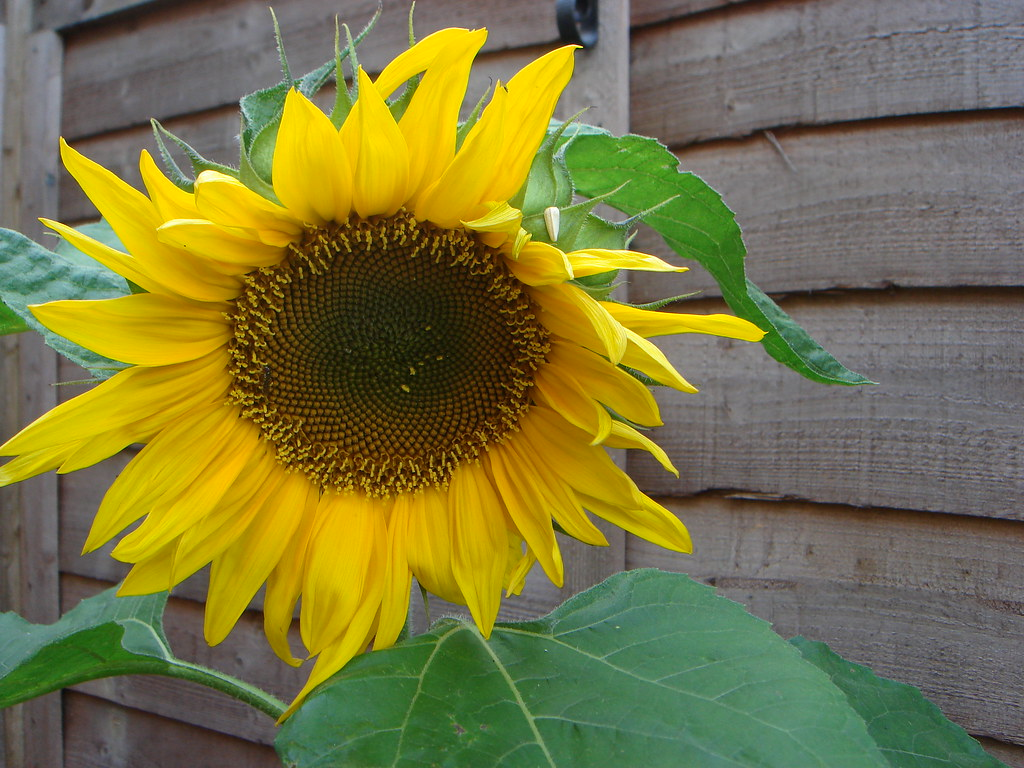
\includegraphics[width=0.38\textwidth]{media/sunflower.jpg}
\caption{\label{sunflower}Distribution of the seeds of a sunflower \cite{simonbrassCCSearch2006}}
\end{wrapfigure}

The distribution of sunflower seeds is an example of the \emph{Fibonacci Sequence}
occuring in a pattern observed in nature (see Figure \ref{sunflower}), the distribution of seeds produces a spiral pattern and the number of clockwise and anti-clockwise spirals that emerge tend to be Fibonacci Numbers. \cite{bohannonSunflowersShowComplex2016}

Although the emergence of the Fibonacci Numbers with respect to the sunflower head and models to explain this emergence is well documented in the literature (see e.g. \cite{ridleyPackingEfficiencySunflower1982,mathaiConstructingSunflowerHead1974,vogelBetterWayConstruct1979}) these have not been reviewed, rather a simple approach to model this phenomena in a way that can be easily programmed with Turtle Graphics (implemented also in \S \ref{turtle}) has been devised,

Assume that the process a sunflower follows when placing seeds is as follows: \footnote{To clarify, this process is merely conjecture, other than seeing a very nice example at \href{https://www.mathsisfun.com/numbers/nature-golden-ratio-fibonacci.html}{\emph{MathIsFun.com}}
\cite{NatureGoldenRatio2018}, no evidence is presented to suggest that this is the way
that sunflowers distribute there seeds.

However the simulations performed within \emph{Julia} are very encouraging and
suggest that this process may offer good insight into the unerlying mechanisms.}

\begin{enumerate}
\item Place a seed
\item Move some small unit away from the origin
\item Rotate some constant angle \(\mathtt{\theta}\)  from the previous seed (with respect to the origin).
\item Repeat this process until a seed hits some outer boundary.
\end{enumerate}

This process can be simulated in Julia as shown in listing
\ref{simulate-sunflower} . When a variety of different angles of rotation are
tried varrious different patterns emerge, such patterns are shown in Figure \ref{simulate-sunflower-image}, choosing an angle of \(\varphi\) produces output as shown in Figure \ref{simulate-sunflower-image}.

A distribution of seeds undder this process would be optimal if the amount of empty space was minimised, spirals, stars and swirls contain patterns that compromise this.



\begin{wrapfigure}{l}{0.5\textwidth}
\centering
\includesvg[width=0.38\textwidth]{media/Outline/golden-flower}
\caption{\label{simulate-sunflower-phi}Optimisation of simulated distribution of Sunflower seeds occurs for \(\theta =2 \varphi  \pi\) as described in section \ref{sunflower-example} and listing \ref{simulate-sunflower}}
\end{wrapfigure}

To minimize this, the proportion of the circle traversed in step 3 must be an
irrational number, however this alone is not sufficent, the decimal values must
also be not to approximated by a rational number, for example
\cite{NatureGoldenRatio2018}:

\begin{itemize}
\item \(\pi \mod 1 \approx \frac{1}{7}=0.71428571428\)
\item \(e \mod 1 \approx \frac{5}{7}= 0.142857142857\)
\end{itemize}

It can be seen by simulation that \(\phi\) and \(\psi\) (because \(\phi \mod 1 =
\psi\)) are solutions to this optimisation problem as shown in Figure
\ref{simulate-sunflower-phi}, this solution is unstable, a very minor change to the
value will result in patterns re-emerging in the distribution. \footnote{An early goal of this project was to demonstrate that \(\theta = \varphi\) had the greatest number of seeds, ideally this would have been implemented using a box-counting method but difficulties in applying this were encountered and so this was not undertaken.}

The bottom right spiral in Figure \ref{simulate-sunflower-image} has a ratio of rotation of \(\frac{1}{\pi}\), the spirals look similar to one direction of the spirals occuring in Figure \ref{simulate-sunflower-phi}, it is not clear if there is any significance to this similarity.

\begin{listing}[htbp]
\begin{minted}[]{julia}
φ = 1.61803398875
ψ = φ^-1
ψ = 0.61803398875
function sfSeeds(ratio)
♘ = Turtle()
    for θ in [(ratio*2*π)*i for i in 1:3000]
        gsave()
        scale(0.05)
        rotate(θ)
#        Pencolor(♘, rand(1)[1], rand(1)[1], rand(1)[1])
        Forward(♘, 1)
        Rectangle(♘, 50, 50)
        grestore()
    end
    label = string("Ratio = ", round(ratio, digits = 8))
    textcentered(label, 100, 200)
end
@svg begin
    sfSeeds(φ)
end 600 600
\end{minted}
\caption{\label{simulate-sunflower}Simulation of the distribution of sunflowers as described in section \ref{sunflower-example}}
\end{listing}

\begin{figure}[htbp]
\centering
\includegraphics[width=9cm]{media/Outline/sunflower-spirals-montage.png}
\caption{\label{simulate-sunflower-image}Simulated Distribution of Sunflower seeds as described in section \ref{sunflower-example} and listing \ref{simulate-sunflower}}
\end{figure}
\section{Julia Sets\hfill{}\textsc{Ryan}}
\label{sec:orgd08e015}
\subsection{Introduction}
\label{sec:org55950cd}
Julia sets provide an example of a family of very complex structures that emerge from a very simple mathematical processes.
\subsection{Motivation}
\label{sec:org45f9a04}
Consider the iterative process \(x \rightarrow x^{2}, \enspace x \in \mathbb{R}\),
for values of \(x>1\) this process will diverge and for \(x<1\) it will converge.

The iterative process \(z \rightarrow z^{2}, \enspace z \in \mathbb{C}\),
for values of \(\left\lvert z \right\rvert >1\) diverges and for \(\left\lvert z \right\rvert <1\) it will converge, this is visualized in \ref{py-circle-plot}

This can be generalised, consider:

\begin{itemize}
\item The complex plane for \(\left\lvert z \right\rvert \leq 1\)
\item Some function \(f_{c}(z) = z^{2} + c, \quad c \leq 1 \in \mathbb{C}\) that can be used to iterate with
\end{itemize}

Every value on that plane will belong to one of the two following sets

\begin{itemize}
\item \(P_{c}\)
\begin{itemize}
\item The set of values on the plane that converge to zero (prisoners)
\item Define \(Q^{(k)}_{c}\) to be the the set of values confirmed as prisoners after \(k\) iterations of \(f_{c}\)
\begin{itemize}
\item this implies \(\lim_{k \rightarrow \infty} \left[ Q^{(k)}_{c}  \right] = P_{c}\)
\end{itemize}
\end{itemize}
\item \(E_{c}\)
\begin{itemize}
\item The set of values on the plane that tend to \(\infty\) (escapees)
\end{itemize}
\end{itemize}

In the case of \(f_{0}(z) = z^{2}\) all values \(\left\lvert z  \right \rvert \leq 1\) are bounded with \(\left\lvert z  \right \rvert = 1\) being an unstable stationary circle, but for different iterative functions like \(f_{1}(z) = z^{2} - 1\) the circle of convergence distorts to a fractal pattern, the set of all points on the boundary of convergence is said to be the \emph{Julia Set} \cite[Ch. 14]{peitgenChaosFractalsNew2004}.

\subsection{Plotting the Sets}
\label{sec:org4a2c5f2}
To implement this test we'll consider a function called \texttt{escape\_test} that applies an
iteration (in this case \(f_{0}: z \rightarrow z^{2}\)) until that value diverges or converges. \footnote{This technique was adapted from Chapter 7 of \emph{Math adventures with Python} \cite{farrellMathAdventuresPython2019}}


\begin{figure}[htbp]
\centering
\includesvg[width=0.38\textwidth]{media/Outline/julia-1}
\caption{\label{py-jl-1-plot}Circle of Convergence for \(f_{0}: z \rightarrow z^{2} - 1\)}
\end{figure}


While iterating with \(f_{c}\) once \(\left\lvert z \right\rvert >
\mathrm{max}\left(\left\{c, 2\right\}\right)\), the value must diverge because
\(\left\lvert c \right\rvert \leq 1\), so rather than record whether or not the
value converges or diverges, the \texttt{escape\_test} can instead record the number of
iterations \((k)\) until the value has crossed that boundary and this will provide
a measurement of the rate of divergence.

The \texttt{escape\_test} function can then be mapped over a matrix, where each element
of that matrix is in turn mapped to a point on the Cartesian Plane, the resulting matrix
can be visualised as an image, this is implemented in listing
\ref{py-circle-code} and the corresponding output shown in \ref{py-circle-plot}.

Observe that the absoluve value was not used in \ref{py-circle-code} (or below in \S
\ref{dim-julia} ), this is because a \texttt{sqrt} is a costly operation that can be avoided
by comparing two squares, this is important when multiple iterations over large
matrices are required, this accounted for as much as 50\% of the time required to
generate the data using listing \ref{definition} in \S \ref{dim-julia}.



\newpage
\begin{listing}[htbp]
\begin{minted}[]{python}
from math import sqrt
def magnitude(z):
    # return sqrt(z[0]**2 + z[1]**2)
    x = z[0]
    y = z[1]
    return sqrt(sum(map(lambda x: x**2, [x, y])))

def cAdd(a, b):
    x = a[0] + b[0]
    y = a[1] + b[1]
    return [x, y]


def cMult(u, v):
    x = u[0]*v[0]-u[1]*v[1]
    y = u[1]*v[0]+u[0]*v[1]
    return [x, y]
\end{minted}
\caption{\label{complex-vec}Defining Complex Operations with vectors}
\end{listing}

\begin{listing}[htbp]
\begin{minted}[]{python}
%matplotlib inline
%config InlineBackend.figure_format = 'svg'
import numpy as np
def escape_test(z, num):
    ''' runs the process num amount of times and returns the count of
    divergence'''
    c = [0, 0]
    count = 0
    z1 = z  #Remember the original value that we are working with
    # Iterate num times
    while count <= num:
        dist = sum([n**2 for n in z1])
        distc = sum([n**2 for n in c])
        # check for divergence
        if dist > max(2, distc):
            #return the step it diverged on
            return count
        #iterate z
        z1 = cAdd(cMult(z1, z1), c)
        count+=1
        #if z hasn't diverged by the end
    return num



p = 0.25 #horizontal, vertical, pinch (zoom)
res = 200
h = res/2
v = res/2

pic = np.zeros([res, res])
for i in range(pic.shape[0]):
    for j in range(pic.shape[1]):
        x = (j - h)/(p*res)
        y = (i-v)/(p*res)
        z = [x, y]
        col = escape_test(z, 100)
        pic[i, j] = col

import matplotlib.pyplot as plt

plt.axis('off')
plt.imshow(pic)
# plt.show()

\end{minted}
\caption{\label{py-circle-code}Circle of Convergence of \(z\) under recursion}
\end{listing}


\begin{wrapfigure}{l}{0.5\textwidth}
\centering
\includesvg[width=0.25\textwidth]{media/Outline/circle-of-convergence}
\caption{\label{py-circle-plot}Circle of Convergence for \(f_{0}: z \rightarrow z^{2}\)}
\end{wrapfigure}

The resulting circle in Figure \ref{py-circle-plot} is precisely what would be expected, verifying this approach.
Consider now the result if this same procedure was applied to a slightly different function, for example the following functions:

\begin{align*}
f_{1}&: z \rightarrow
z^{2} - 1 \\
f_{\frac{1}{4} + \frac{i}{2}}&: z
\rightarrow z^{2} + (\frac{1}{4} + \frac{i}{2})
\end{align*}

The result is
remarkably unexpected, as shown in Figures \ref{py-jl-1-plot} and \ref{py-jl-rab-plot}.




To investigate this further consider the
more general function:

\begin{align}
f_{0.8 e^{\pi i \tau}}: z \rightarrow z^{2} + 0.8 e^{\pi
i \tau}, \enspace \tau \in \mathbb{R}
\end{align}

Many fractals can be generated using
this set by varying the value of \(\tau\)\footnote{This approach was inspired by an animation on the \emph{Julia Set} Wikipedia article \cite{JuliaSet2020}}. \emph{Julia} will be used to implement this due to performance constraints. These images can be
generated in \emph{Julia} in a similar fashion as before, with the specifics shown in
listing \ref{julia-gen-fracs}. The \texttt{GR} package appears to be the best plotting
library performance wise and so was used to save corresponding images to disc,
this is demonstrated in listing \ref{GR-save} where 1200 pictures at a 2.25 MP
resolution were produced. \footnote{This took about 30 minutes on an Intel I7-7700 with 32GB memory using \emph{Julia 1.5.2}}


\begin{wrapfigure}{l}{0.5\textwidth}
\centering
\includesvg[width=0.38 \textwidth]{media/Outline/julia-rab}
\caption{\label{py-jl-rab-plot}Boundary of Convergence for \(f_{\frac{1}{4} + \frac{i}{2}}: z \rightarrow z^{2} + \frac{1}{4} + \frac{i}{2}\), the figure was contrasted using \emph{ImageMagick} to highlight the complex boundary}
\end{wrapfigure}

A subset of these images can be combined using \emph{ImageMagick} and \texttt{bash} to
create a collage, \emph{ImageMagick} can also be used to produce an animation but it often
fails and a superior approach is to use \texttt{ffmpeg}, this is demonstrated in
listing \ref{bash-frac-join}, the collage is shown in Figure \ref{montage-frac}.

\begin{listing}[htbp]
\begin{minted}[]{julia}
# * Define the Julia Set
"""
Determine whether or not a value will converge under iteration
"""
function juliaSet(z, num, my_func)
    count = 1
    # Remember the value of z
    z1 = z
    # Iterate num times
    while count ≤ num
        # check for divergence
        if abs(z1)>2
            return Int(count)
        end
        #iterate z
        z1 = my_func(z1) # + z
        count=count+1
    end
        #if z hasn't diverged by the end
    return Int(num)
end

# * Make a Picture
"""
Loop over a matrix and apply apply the julia-set function to
the corresponding complex value
"""
function make_picture(width, height, my_func)
    pic_mat = zeros(width, height)
    zoom = 0.3
    for i in 1:size(pic_mat)[1]
        for j in 1:size(pic_mat)[2]
            x = (j-width/2)/(width*zoom)
            y = (i-height/2)/(height*zoom)
            pic_mat[i,j] = juliaSet(x+y*im, 256, my_func)
        end
    end
    return pic_mat
end

\end{minted}
\caption{\label{julia-gen-fracs}Produce a series of fractals using julia}
\end{listing}

\begin{listing}[htbp]
\begin{minted}[]{julia}
# * Use GR to Save many images
  ## GR is faster than PyPlot
using GR
function save_images(count, res)
    try
        mkdir("/tmp/gifs")
    catch
    end
    j = 1
    for i in (1:count)/(40*2*π)
        j = j + 1
        GR.imshow(make_picture(res, res, z -> z^2 + 0.8*exp(i*im*9/2))) # PyPlot uses interpolation = "None"
        name = string("/tmp/gifs/j", lpad(j, 5, "0"), ".png")
        GR.savefig(name)
    end
end

save_images(1200, 1500) # Number  and Res
\end{minted}
\caption{\label{GR-save}Generate and save the images with GR}
\end{listing}

\begin{listing}[htbp]
\begin{minted}[]{bash}
# Use montage multiple times to get recursion for fun
montage (ls *png | sed -n '1p;0~600p') 0a.png
montage (ls *png | sed -n '1p;0~100p') a.png
montage (ls *png | sed -n '1p;0~50p') -geometry 1000x1000  a.png

# Use ImageMagick to Produce a gif (unreliable)
convert -delay 10 *.png 0.gif

# Use FFMpeg to produce a Gif instead
ffmpeg                    \
    -framerate 60         \
    -pattern_type glob    \
    -i '*.png'            \
    -r 15                 \
    out.mov


\end{minted}
\caption{\label{bash-frac-join}Using \texttt{bash}, \texttt{ffmpeg} and \emph{ImageMagick} to combine the images and produce an animation.}
\end{listing}

\begin{figure}[htbp]
\centering
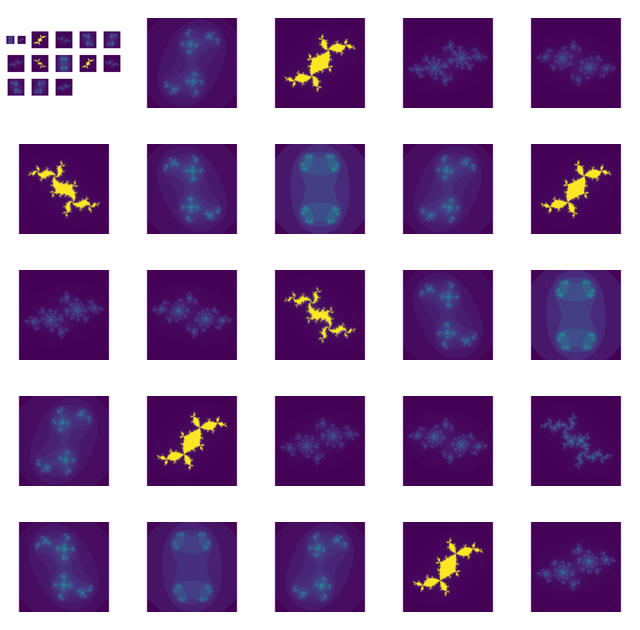
\includegraphics[width=1.0\textwidth]{media/Outline/many_julia_fractals_around_circle.png}
\caption{\label{montage-frac}Various fracals corresponding to \(f_{0.8 e^{\pi i \tau}}\)}
\end{figure}

\subsection{Dimension of the Julia Set}
\label{dim-julia}
The Julia Set is defined as the boundary between which values diverge and
converge on the complex plane
\cite[\S 14.1]{falconerFractalGeometryMathematical2003b}, this means a matrix
representing such a fractal must only have values along this boundary. This can
be acheived by looping over every element of a matrix and replacing each value
with 0 if it is surrounded on all sides values.

To implement this for a boolean matrix a function could consider if immediately
adjacent elements sum to 9, that point should be set to 0 if this is true
because it does not represent a boundary. This is implemented in \ref{outline-func}
and although this will not perfectly trace the outline of a fractal like the
\emph{Julia Set}, it is expected that this approach will not introduce bias and so
the impact on accuraccy will be constant for \emph{Julia Sets} accross all scales of
resolution.

\begin{listing}[htbp]
\begin{minted}[]{julia}
function outline(mat)
    work_mat = copy(mat)
    for col in 2:(size(mat)[2]-1)
        for row in 2:(size(mat)[1]-1)
            ## Make the inside 0, we only want the outline
            neighbourhood = mat[row-1:row+1,col-1:col+1]
            if sum(neighbourhood) >= 9 # 9 squares
                work_mat[row,col] = 0
            end
        end
    end
    return work_mat
end
\end{minted}
\caption{\label{outline-func}A function to set all values of matrix, that do not represent the boundary of a shape, to zero. This is designed for a boolean matrix and works by summing the neighbourhood of an element, if that neighbourhood is greater than 9 (indicating that all values surrounding the point contain an element), the value is set to 1.}
\end{listing}

In order to measure the dimension of the \emph{Julia Set} it is necessary to generate
a representation of the fractal at two scales, compare them and then
measure the corresponding dimension value as in \S \ref{gen-self-sim-frac}. The julia set
is a non self-similar fractal and so it is not immediately clear whether or not
the dimension will be constant at all scales, to determine whether or not the
dimension is constant at various scales it can be convenient to plot the log
transformed scaling factor and measures and inspect whether or not the points
form a linear relationship, the slope of such a relationship will be the
dimension as discussed in \S \ref{sans-self}.

To implement this all the functions necessary to build the fractals were placed
into a seperate script \texttt{julia-set-functions.jl} which is shown in \S
and this script was included into a working script
\texttt{julia-set-dimensions.jl} by using the following line:

\begin{minted}[]{julia}
@time include("./Julia-Set-Dimensions-functions.jl")
\end{minted}



\begin{figure}[htbp]
\centering
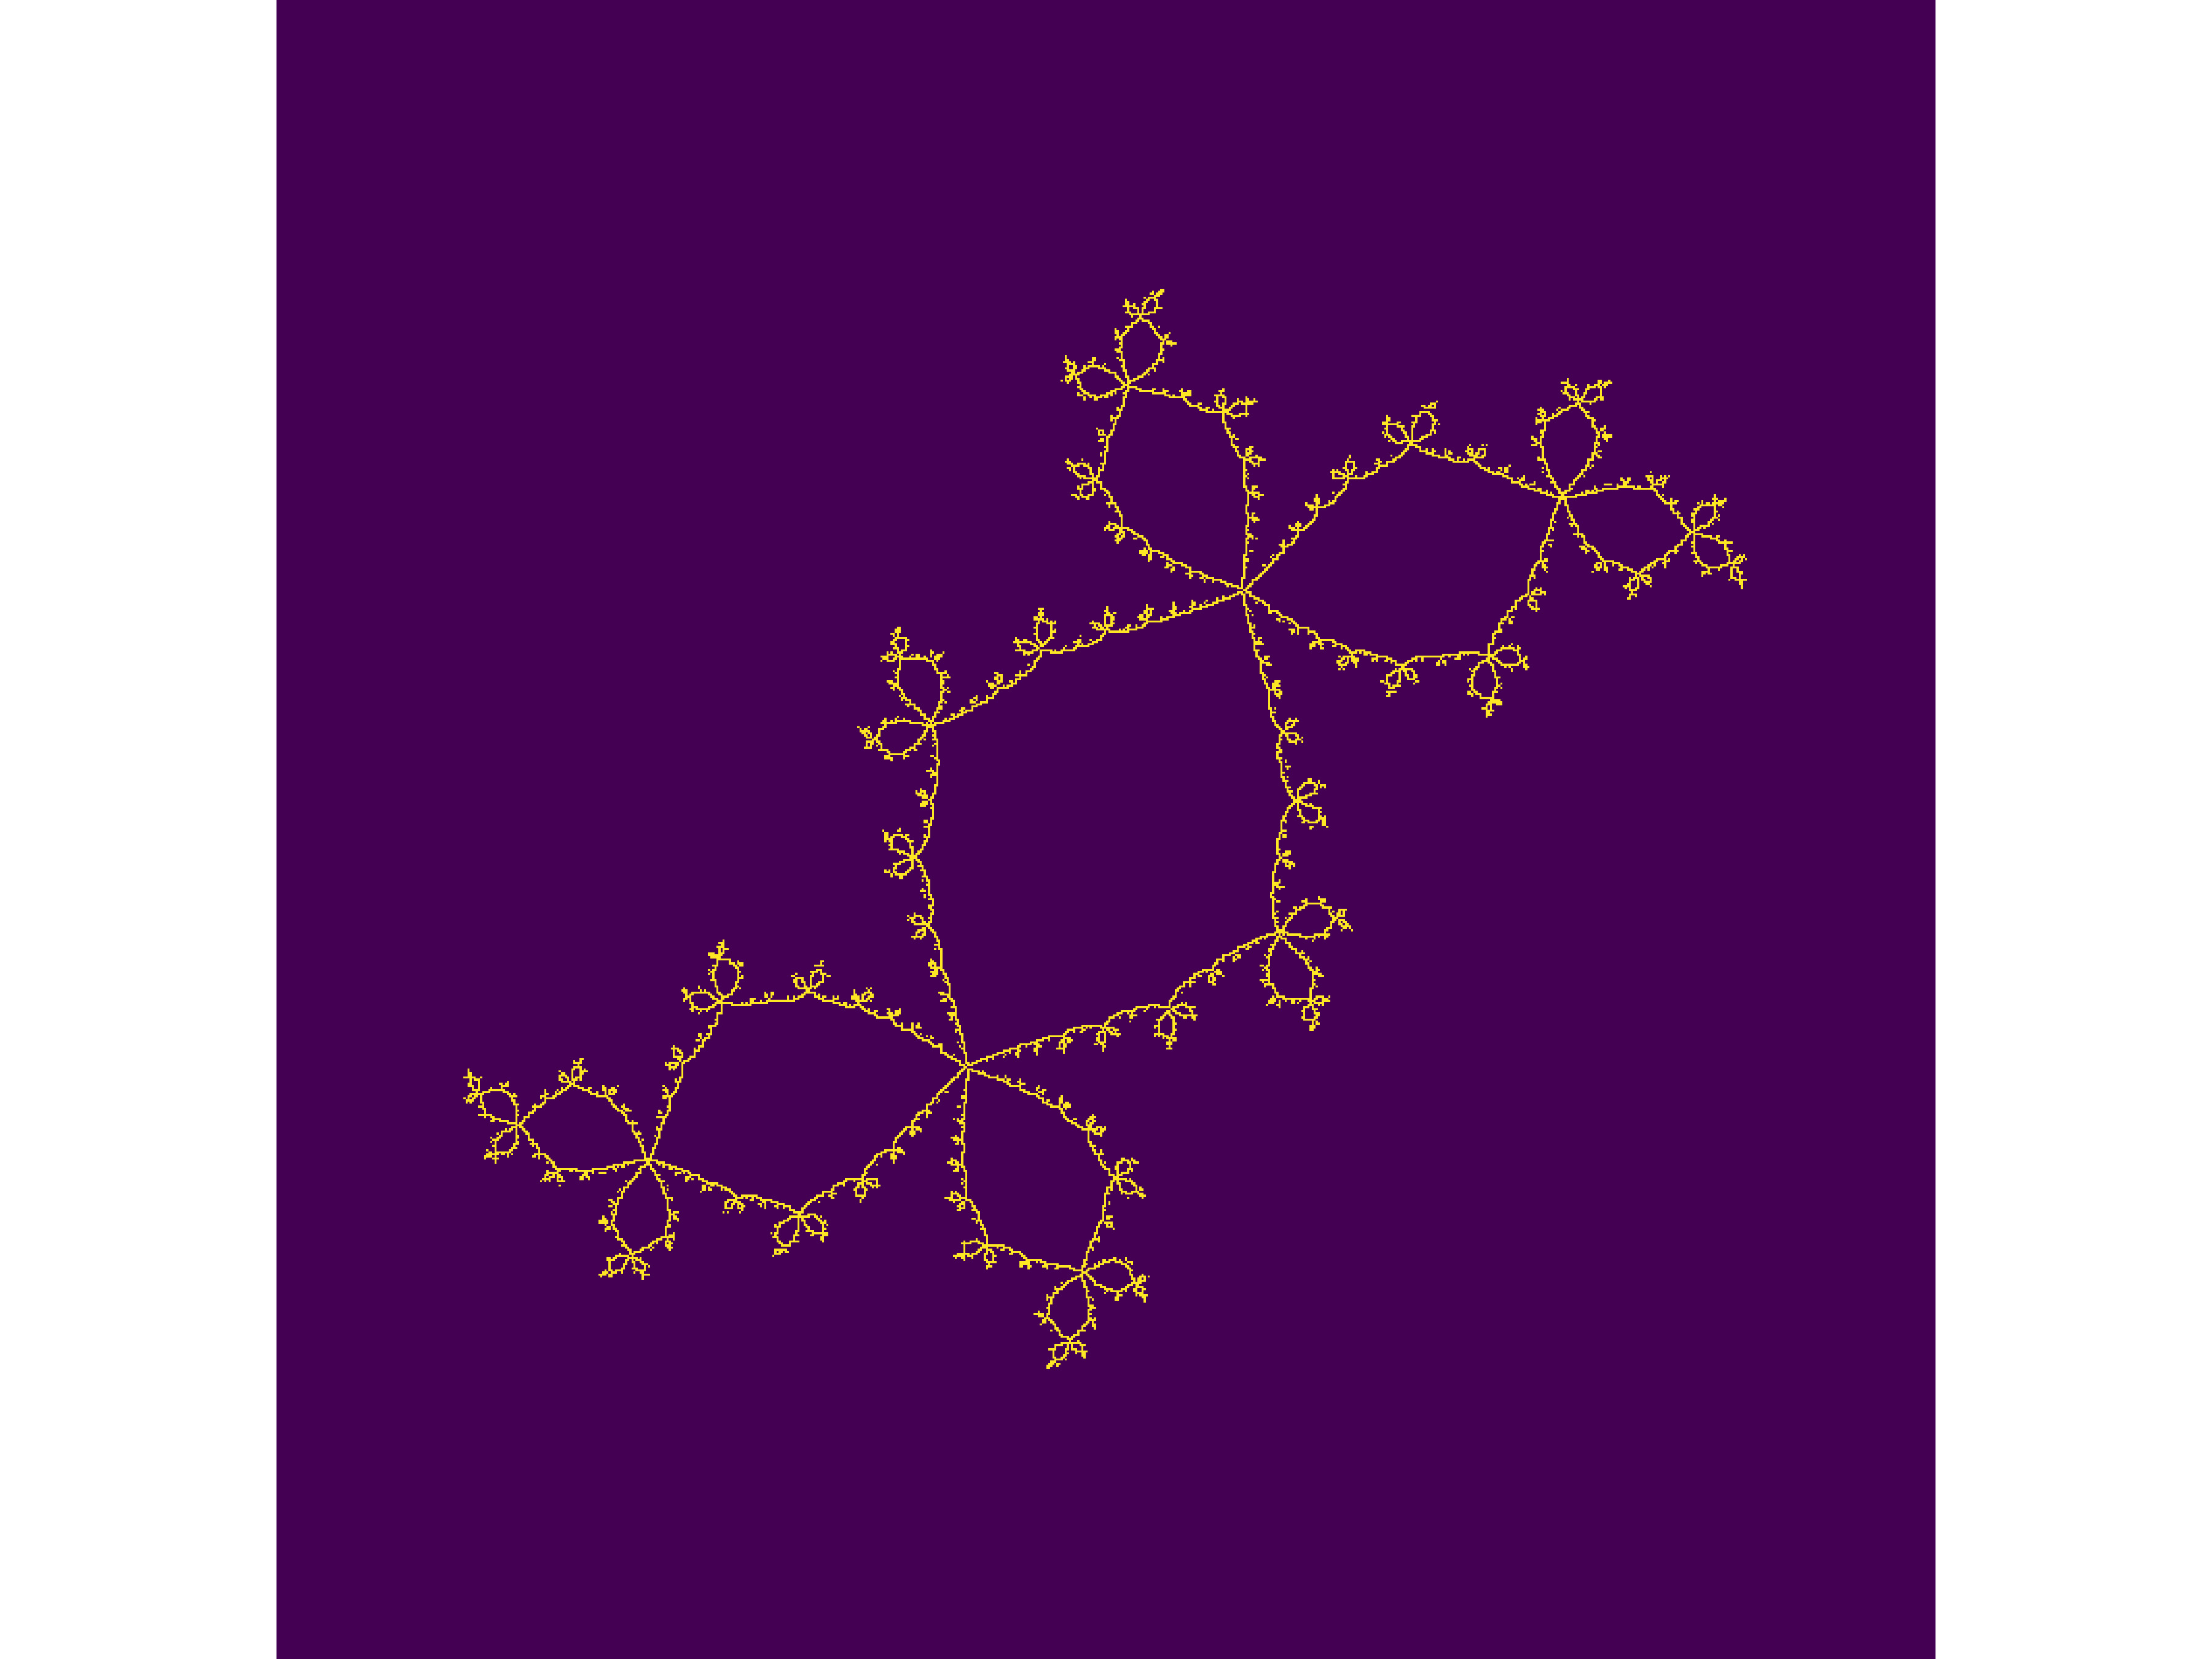
\includegraphics[width=0.85\textwidth]{media/outline-rabbit.png}
\caption{\label{fig:julia-rab}Image of the Doudy Rabbit, the julia set corresponding to the iteration of \(z \leftarrow z^{2} -0.123+0.745i\) produced by \emph{Julia} in listing \ref{dimensions-julia-set}.}
\end{figure}


\newpage
\begin{listing}[htbp]
\begin{minted}[]{julia}
@time include("./Julia-Set-Dimensions-functions.jl")

#### Investigate Plot #######################################
test_mat = make_picture(800,800, z -> z^2 + -0.123+0.745*im)

#Inspect
GR.imshow(test_mat) # PyPlot uses interpolation = "None"
# Outline
test_mat = outline(test_mat)
#Inspect
GR.imshow(test_mat) # PyPlot uses interpolation = "None"
## Return the perimeter
sum(test_mat)

# Take a measurement at a point
mat2 = outline(make_picture(9000,9000, f))
l2   = sum(mat2)
size2 = size(mat2)[1]
mat1 = outline(make_picture(10000,10000, f))
l1   = sum(mat1)
size1 = size(mat1)[1]
log(l2/l1)/log(size2/size1)
# 1.3934 Douady Rabbit

# Take a measurement using LInear Regression
using CSV
@time data=scaleAndMeasure(900, 1000 , 4, f)
# CSV.read("./julia-set-dimensions.csv", data)
# data = CSV.read("./julia-set-dimensions.csv")
data.scale = [log(i) for i in data.scale]
data.mass  = [log(i) for i in data.mass]
mod   = lm(@formula(mass ~ scale), data)
p = Gadfly.plot(data, x=:scale, y=:mass, Geom.point)

print("the slope is $(round(coef(mod)[2], sigdigits=4))")
print(mod)
print("\n")
return mod

a = SharedArray{Float64}(10)
@distributed for i = 1:10
    a[i] = i
end

#------------------------------------------------------------
# julia> return mod
#
# mass ~ 0 + scale
#
# Coefficients:
# ────────────────────────────────────────────────────────────────────
#          Coef.   Std. Error        t  Pr(>|t|)  Lower 95%  Upper 95%
# ────────────────────────────────────────────────────────────────────
# scale  1.28358  0.000497296  2581.11     <1e-9    1.28199    1.28516
# ────────────────────────────────────────────────────────────────────

\end{minted}
\caption{\label{dimensions-julia-set}Functions used by listing \ref{dimensions-julia-set}}
\end{listing}

The working script to measure the dimension of the Julia Set is shown in listing
\ref{dimensions-julia-set}. This script generates fractals of the \emph{Julia Set}
corresponding to \(z \leftarrow z^{2} -0.123+0.745i\) for a variety of different
scales, at each scale the measure of the fractal is recorded and by running the code in listing \ref{dimensions-julia-set}
for scales from 9000 to 10000 and leaving it for an hour, the following
table of values is returned:

\begin{center}
\begin{tabular}{rr}
\textbf{\emph{Scale}} & \textbf{\emph{Mass}}\\
\hline
500 & 4834.0\\
563 & 5754.0\\
625 & 6640.0\\
688 & 7584.0\\
750 & 8418.0\\
813 & 9550.0\\
875 & 10554.0\\
938 & 11710.0\\
1000 & 12744.0\\
\end{tabular}

\end{center}


Using this technique the dimension of the Julia Set converges very slowly and
the code can take a very long time to run, and has a tendency to cause crashes,
likely due to the large amounts of memory required, the values produced took
about one hour to produce.

Linear Regression can be performed against these values using \textbf{\emph{R}} \footnote{The could just as well have been done inside Julia, \textbf{\emph{R}} was chosen simply because \texttt{ggplot} produces very nice plots.}

\begin{minted}[]{r}
scale   <- c(500, 563, 625, 688, 750, 813, 875, 938, 1000)
measure <- c(  4834, 5754, 6640, 7584, 8418, 9550, 10554, 11710, 12744)
data <- data.frame(scale, measure)

lm(log(measure) ~ 0 + log(scale), data)$coefficients # set 0 intercept

#------------------------------------------------------------
# 1.36720041333112
\end{minted}

This shows that the value returned is 1.37 which is very close to the value of
1.39 which is reported in the literature
\cite{mcmullenHausdorffDimensionConformal1998}. A plot can be produced (shown in Figure \ref{fig:lin-reg-dim}) by using the following \textbf{\emph{R}} code:

\begin{minted}[]{r}
library(ggplot2)
ggplot(data, aes(x = log(measure), y = log(scale))) +
  geom_point(size = 6, col = 'red') +
  geom_smooth(method = 'lm') +
  theme_bw() +
  labs(x = "log Measure", y = "log Scale",
       title = "Comparison of Scale and Measure of Julia Set", subtitle = "Douady Rabbit")
\end{minted}

\begin{figure}[htbp]
\centering
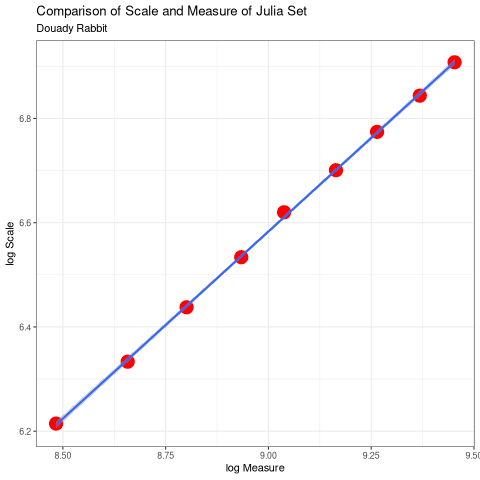
\includegraphics[width=0.45\textwidth]{media/r-ggplot-linear-reg-julia.png}
\caption{\label{fig:lin-reg-dim}Log Scaled Linear Regression of various scales of the julia set.}
\end{figure}


Inspecting the behaviour ofthe log transformed scale and measure in Figure
\ref{fig:lin-reg-dim} indicates that there is a very linear relationship between these
variables and so even though this julia set does not appear to demonstrate
simple self-similarity, it appears to be a figure with a constant dimension
across scales.
\section{Mandelbrot Set\hfill{}\textsc{Ryan}}
\label{mandlebrot-set}
Investigating the Julia Set in Figure \ref{montage-frac}, a natural question arises, \emph{which values of \(c\)
produce a fractal that is an open disc or a closed disc}. If an arbitrary complex value \(\left\lvert \gamma \right \rvert < 1\)
is chosen to produce the julia set \(f_{\gamma}\), that value is said to belong to the Mandelbrot set if the corresponding \emph{Julia Set} is a closed disc \cite[Ch. 14]{peitgenChaosFractalsNew2004}.
\(P\) is closed we this value is defined as belonging to the \emph{Mandelbrot} set.

It can be shown, that a value \(z_{0}\) is interior to the \emph{Mandelbrot Set} if \(f_{z_{0}}\) is interior to the julia set and hence this problem is equivalent to re-implementing the previous strategy such that \(z \rightarrow z^{2} + z_{0}\) where \(z_{0}\) is unchanging or more clearly as a seqeuence:

\begin{align}
z_{n+1} &= z^{2}_n + c \label{eq:mb-sequence} \\
z_{0}   &= c
\end{align}

This strategy is implemented in listing and produces the output shown in Figure \ref{mandelbrot-py-pic}.


\begin{figure}[htbp]
\centering
\includesvg[width=0.38\textwidth]{media/Outline/mandelbrot-py}
\caption{\label{mandelbrot-py-pic}Mandelbrot Set produced in \emph{Python} as shown in listing \ref{py-mandelbrot-code}}
\end{figure}

\begin{listing}[htbp]
\begin{minted}[]{python}
%matplotlib inline
%config InlineBackend.figure_format = 'svg'
import numpy as np

def mandelbrot(z, num):
    ''' runs the process num amount of times and returns the count of
    divergence'''
    count = 0
    # Define z1 as z
    z1 = z
    # Iterate num times
    while count <= num:
        # check for divergence
        if magnitude(z1) > 2.0:
            #return the step it diverged on
            return count
        #iterate z
        z1 = cAdd(cMult(z1, z1),z)
        count+=1
        #if z hasn't diverged by the end
    return num

p = 0.25 # horizontal, vertical, pinch (zoom)
res = 200
h = res/2
v = res/2

pic = np.zeros([res, res])
for i in range(pic.shape[0]):
    for j in range(pic.shape[1]):
        x = (j - h)/(p*res)
        y = (i-v)/(p*res)
        z = [x, y]
        col = mandelbrot(z, 100)
        pic[i, j] = col

import matplotlib.pyplot as plt
plt.imshow(pic)
# plt.show()
\end{minted}
\caption{\label{py-mandelbrot-code}All values of \(c\) that lead to a closed \emph{Julia-set}}
\end{listing}


This output although remarkable is however fairly undetailed, by using \emph{Julia} a much
larger image can be produced, in \emph{Julia} producing a 4 GB, 400 MP image can be done in little time
(about 10 minutes on my system), this is demonstrated in listing \ref{julia-large-mandelbrot}
and a screenshot of the corresponding FITS image is shown in listing \ref{mandelbrot-screen}.

\newpage
\begin{listing}[htbp]
\begin{minted}[]{julia}
function mandelbrot(z, num, my_func)
    count = 1
    # Define z1 as z
    z1 = z
    # Iterate num times
    while count ≤ num
        # check for divergence
        if abs(z1)>2
            return Int(count)
        end
        #iterate z
        z1 = my_func(z1) + z
        count=count+1
    end
        #if z hasn't diverged by the end
    return Int(num)
end

function make_picture(width, height, my_func)
    pic_mat = zeros(width, height)
    for i in 1:size(pic_mat)[1]
        for j in 1:size(pic_mat)[2]
            x = j/width
            y = i/height
            pic_mat[i,j] = mandelbrot(x+y*im, 99, my_func)
        end
    end
    return pic_mat
end


using FITSIO
function save_picture(filename, matrix)
    f = FITS(filename, "w");
    # data = reshape(1:100, 5, 20)
    # data = pic_mat
    write(f, matrix)  # Write a new image extension with the data

    data = Dict("col1"=>[1., 2., 3.], "col2"=>[1, 2, 3]);
    write(f, data)  # write a new binary table to a new extension

    close(f)
end

# * Save Picture
#------------------------------------------------------------
my_pic = make_picture(20000, 20000, z -> z^2) 2000^2 is 4 GB
save_picture("/tmp/a.fits", my_pic)

\end{minted}
\caption{\label{julia-large-mandelbrot}Generate High Resolution Mandelbrot Set and Export as Fits Image using Julia.}
\end{listing}

\begin{figure}[htbp]
\centering
\includegraphics[width=1\textwidth]{media/Outline/_20200828_233844screenshot.png}
\caption{\label{mandelbrot-screen}Screenshot of Mandelbrot FITS image produced by listing \ref{julia-large-mandelbrot}}
\end{figure}


The dimension of the mandelbrot set is 2 \cite{bownScienceMandelbrotSet} and can be measured using the exact same strategy as \S \ref{dim-julia}. \footnote{As a matter of fact it would only be necessary to uncomment the end of line 40 of the listing provided in \S \ref{julia-set-functions-script} and use the function \texttt{juliaSet(z, z -> z\textasciicircum{}2)}} The Mandelbrot set is extraodinarily complex and actually contains many of the patterns of various Julia Sets within it \cite[Ch. 14]{peitgenChaosFractalsNew2004}.
\section{Conclusion\hfill{}\textsc{Ryan:James}}
\label{sec:orgd414e7e}
Fractals are complex shapes that may or may not exhibit self similarity and often arise from natural phenomena. They are hard to define in a way that captures all potential edge cases. One important feature of fractals is the dimension of the complex shape, they are not simple finite shapes and so there dimension is usually higher than what might be anticipated by considering the corresponding the dimension of a shape that may approximate the general figure.

This concept of dimension can be extended to shapes that do not exhibit clear self-similarity by using linear regression, this includes particularly complex fractals such as the Mandelbrot Set.

Simple processes that involve recursion can lead to the emergence of patterns that are fractals, these fractals can often include other characteristic properties that involve values such as the golden ratio and Fibonacci Numbers.

 \appendix 
\section{Appendix}
\label{appendix}
So unless code contributes directly to the discussion we'll put it in the appendix.
\subsection{Code Listings\hfill{}\textsc{Ryan}}
\label{sec:orgecefc5f}
The code listings used to produce Sierpinski's Carpet and Cantor's Dust are provided in listings \ref{l-s-carpet} and \ref{l-cant-dust} respectively.

\begin{listing}[htbp]
\begin{minted}[]{julia}
#------------------------------------------------------------
#--- Function -----------------------------------------------
#------------------------------------------------------------

function carpet(ICMat, width)
    B = ICMat
    h  = size(B)[1]
    w  = size(B)[2]
    Z  = zeros(Int, h, w)
    B = [B B B;
         B Z B;
         B B B]
    if (3*w)<width
        B = carpet(B, width)
    end
    return B
end

#------------------------------------------------------------
#-- Plot ----------------------------------------------------
#------------------------------------------------------------
using GR, Plots
gr() # Set Plots backend as GR

(mat = carpet(fill(1, 1, 1), 9^2)) |> size
p1 = GR.imshow(mat)

#------------------------------------------------------------
#-- Dimension -----------------------------------------------
#------------------------------------------------------------
mat2 = carpet(fill(1, 1, 1), 1000)
l2   = sum(mat2)
size2 = size(mat2)[1]
mat1 = carpet(fill(1, 1, 1), 500)
l1   = sum(mat1)
size1 = size(mat1)[1]

#------------------------------------------------------------
## julia> log(l2/l1)/log(size2/size1)
## 1.89
\end{minted}
\caption{\label{l-s-carpet}Function to produce Sierpinski's carpet, shown in Figure \ref{fig:square-carpet}}
\end{listing}


\newpage
\begin{listing}[htbp]
\begin{minted}[]{julia}
#------------------------------------------------------------
#--- Function -----------------------------------------------
#------------------------------------------------------------

function dust(ICMat, width)
    B = ICMat
    h  = size(B)[1]
    w  = size(B)[2]
    Z  = zeros(Int, h, w)
    B = [Z Z B Z;
         B Z Z Z;
         Z Z Z B;
         Z B Z Z]
    if (3*w)<width
        B = dust(B, width)
    end
    return B
end

#------------------------------------------------------------
#-- Plot ----------------------------------------------------
#------------------------------------------------------------
using GR, Plots
gr() # Set Plots backend as GR

(mat = dust(fill(1, 1, 1), 9^2)) |> size
p1 = GR.imshow(mat)


#------------------------------------------------------------
#-- Dimension -----------------------------------------------
#------------------------------------------------------------
mat2 = dust(fill(1, 1, 1), 1000)
l2   = sum(mat2)
size2 = size(mat2)[1]
mat1 = dust(fill(1, 1, 1), 500)
l1   = sum(mat1)
size1 = size(mat1)[1]

#------------------------------------------------------------
## julia> log(l2/l1)/log(size2/size1)
## 1.0

\end{minted}
\caption{\label{l-cant-dust}Function to generate Cantor Dust, shown in }
\end{listing}

\subsection{Resources Used for the Hausdorff Dimension\hfill{}\textsc{Ryan}}
\label{haus-resource}
Research for \S on the Hausdorff Dimension proved actually to be quite difficult, while much information is available online, precice and clear explanations of the Hausdorff dimension are difficult to find without scouring texts, the following proved very helpful generally in preparing for this topic and I would strongly recommend these chapters as a starting point for further reading on this topic:

\begin{itemize}
\item Edgar, G. A., \emph{Measure, topology, and fractal geometry} \cite[Ch. 6]{edgarMeasureTopologyFractal2008a}
\item Falconer, K. J., \emph{Fractal geometry: mathematical foundations and applications}  \cite[Ch. 2]{falconerFractalGeometryMathematical2003b}
\item Gouyet, J., \emph{Physics and fractal structures} \cite[\S1.3]{gouyetPhysicsFractalStructures1996}
\item Vicsek, T., \emph{Fractal Growth Phenomena} \cite[Ch. 4]{vicsekFractalGrowthPhenomena1992}
\begin{itemize}
\item See also p 14 specifically
\end{itemize}
\item Tél, T., Gruiz, M., \& Kulacsy, K., \emph{Chaotic dynamics: an introduction based on classical mechanics}  \cite[\S2.1.2]{telChaoticDynamicsIntroduction2006}
\item Peitgen, H., Jürgens, H., \& Saupe, D., \emph{Chaos and fractals: new frontiers of science}  \cite[\S 4.3]{peitgenChaosFractalsNew2004}
\end{itemize}

\subsection{Functions for constructing the Julia Set\hfill{}\textsc{Ryan}}
\label{julia-set-functions-script}
The following functions were saved in a file called:

\begin{itemize}
\item \texttt{@time include("./Julia-Set-Dimensions-functions.jl")}
\end{itemize}

This file was loaded into the current workspace by using the following at the top of a \emph{Julia} script:

\begin{itemize}
\item \texttt{@time include("./Julia-Set-Dimensions-functions.jl")}
\end{itemize}


\begin{minted}[]{julia}
using GR
using DataFrames
using Gadfly
using GLM
using SharedArrays
using Distributed

############################################################
### Julia / MandelBrot Functions ###########################
############################################################

"""
# Julia Set
Returns how many iterations it takes for a value on the complex plane to diverge
under recursion. if `boolQ` is specified as true a 1/0 will be returned to
indicate divergence or convergence.

## Variables
- `z`
  - A value on the complex plane within the unit circle
- `num`
  - A number of iterations to perform before conceding that the value is not
    divergent.
- `my_func`
  - A function to perform on `z`, for a julia set the function will be of the
    form `z -> z^2 + a + im*b`
    - So for example the Douady Rabbit would be described by `z -> z^2 -0.123+0.745*im`
"""
function juliaSet(z, num, my_func, boolQ=true)
    count = 1
    # Define z1 as z
    z1 = z
    # Iterate num times
    while count ≤ num
        # check for divergence
        if real(z1)^2+imag(z1)^2 > 2^2
            if(boolQ) return 0 else return Int(count) end
        end
        #iterate z
        z1 = my_func(z1) # + z
        count=count+1
    end
        #if z hasn't diverged by the end
    if(boolQ) return 1 else return Int(count) end
end


"""
# Mandelbrot Set
Returns how many iterations it takes for a value on the complex plane to diverge
under recursion of \$z \\rightarrow z^2 + z_0\$.

Values that converge represent constants of the julia set that lead to a
connected set. (TODO: Have I got that Vice Versa?)


## Variables
- `z`
  - A value on the complex plane within the unit circle
- `num`
  - A number of iterations to perform before conceding that the value is not
    divergent.
- `boolQ`
  - `true` or `false` value indicating whether or not to return 1/0 values
    indicating divergence or convergence respecitvely or to return the number of
   iterations performed before conceding no divergence.
"""
function mandelbrot(z, num, boolQ = true)
    count = 1
    # Define z1 as z
    z1 = z
    # Iterate num times
    while count ≤ num
        # check for divergence
        if real(z1)^2+imag(z1)^2 > 2^2
            if(boolQ) return 0 else return Int(count) end
        end
        #iterate z
        z1 = z1^2 + z
        count=count+1
    end
        #if z hasn't diverged by the end
    return 1 # Int(num)
    if(boolQ) return 1 else return Int(count) end
end

function test(x, y)
    if(x<1) return x else return y end
end


############################################################
##### Build a Matrix Image #################################
############################################################

"""
# Make a Picture

This maps a function on the complex plane to a matrix where each element of the
matrix corresponds to a single value on the complex plane. The matrix can be
interpreted as a greyscale image.

Inside the function is a `zoom` parameter that can be modified for different
fractals, fur the julia and mandelbrot sets this shouldn't need to be adjusted.

The height and width should be interpreted as resolution of the image.

- `width`
  - width of the output matrix
- `height`
  - height of the output matrix
- `myfunc`
  - Complex Function to apply across the complex plane
"""
function make_picture(width, height, my_func)
    pic_mat = zeros(width, height)
    zoom = 0.3
    for j in 1:size(pic_mat)[2]
        for i in 1:size(pic_mat)[1]
            x = (j-width/2)/(width*zoom)
            y = (i-height/2)/(height*zoom)
            pic_mat[i,j] = juliaSet(x+y*im, 256, my_func)
        end
    end
    return pic_mat
end

############################################################
### Make the Outline ########################################
############################################################

"""
# Outline

Sets all elements with neighbours on all sides to 0.

- `mat`
  - A matrix
    - If this matrix is the convergent values corresponding to a julia set the
      output will be the outline, which is the definition of the julia set.
"""
function outline(mat)
    work_mat = copy(mat)
    for col in 2:(size(mat)[2]-1)
        for row in 2:(size(mat)[1]-1)
            ## Make the inside 0, we only want the outline
            neighbourhood = mat[row-1:row+1,col-1:col+1]
            if sum(neighbourhood) >= 9 # 9 squares
                work_mat[row,col] = 0
            end
        end
    end
    return work_mat
end


############################################################
###### Return many Scaled Values ###########################
############################################################



function scaleAndMeasure(min, max, n, func)
    # The scale is equivalent to the resolution, the initial resolution could be
    # set as 10, 93, 72 or 1, it's arbitrary (previously I had res and scale)
    # #TODO: Prove this

    scale = [Int(ceil(i)) for i in range(min, max, length=n) ]
    mass = pmap(s -> sum(outline(make_picture(Int(s), Int(s), func))) , scale)

    data = DataFrame(scale = scale, mass = mass)
    return data
end

\end{minted}

\subsection{Exponential Generating Functions}
\label{exp-gen-func-fib-seq}
Exponential Generating Functions can be used to find solutions to linear
recurrence relations, Markov Chains and Differential Equaions and may provide
insight into the connections between discrete and continuous process.

We were unable to find time to show generally the relationship between homogenous ODEs and homogenous linear recurrence relations and this work was not directly relevant to this report, it is included in this appendix for reference sake.

\paragraph{Derivative of the Exponential Generating Function}
\label{Derivative-exp-gen-function}
\subparagraph{Base\hfill{}\textsc{Ryan}}
\label{sec:orgc2b8b99}
Differentiating the exponential generating function has the effect of shifting the sequence once to the left: \cite{lehmanReadingsMathematicsComputer2010}

\begin{align}
    f\left( x \right) &= \sum^{\infty}_{n= 0}   \left[ a_n \frac{x^n}{n!} \right] \label{eq:exp-pow-series} \\
f'\left( x \right) &= \frac{\mathrm{d} }{\mathrm{d} x}\left( \sum^{\infty}_{n= 0}   \left[ a_n \frac{x^n}{n!} \right]  \right) \nonumber \\
&= \frac{\mathrm{d}}{\mathrm{d} x} \left( a_0 \frac{x^0}{0!} +  a_1 \frac{x^1}{1!} +  a_2 \frac{x^2}{2!}+  a_3 \frac{x^3}{3! } +  \ldots \frac{x^k}{k!} \right) \nonumber \\
&= \sum^{\infty}_{n= 0}   \left[ \frac{\mathrm{d} }{\mathrm{d} x}\left( a_n \frac{x^n}{n!} \right) \right] \nonumber \\
&= \sum^{\infty}_{n= 0}   {\left[{ \frac{a_n}{{\left({ n- 1 }\right)!}} } x^{n- 1}  \right]} \nonumber \\
\implies f'(x) &= \sum^{\infty}_{n= 1}   {\left[{ \frac{x^n}{n!}a_{n+  1} }\right]} \label{eq:exp-pow-series-sol}
\end{align}

\subparagraph{Bridge\hfill{}\textsc{James}}
\label{sec:org58c9277}
This can be shown for all derivatives by way of induction, for

\begin{align}
f^{(k)}\left(x\right) = \sum_{n=k}^\infty\frac{a_{n+k}\cdot x^n}{n!} \quad \text{for}~k \ge 0
\end{align}

Assume that \(f^{(k)}\left(x\right) = \sum_{n=k}^\infty\frac{a_{n+k}\cdot x^n}{n!}\)

Using this assumption, prove for the next element \(k+1\)

We need \(f^{(k+1)}(x) = \sum_{n=k+1}^\infty\frac{a_{n+k+1}\cdot x^n}{n!}\)

\begin{align*}
    \text{LHS} &= f^{(k+1)}(x)\\
    &= \frac{\mathrm{d}}{\mathrm{d}x}\left(f^{(k)}(x)\right)\\
    &= \frac{\mathrm{d}}{\mathrm{d}x}\left(\sum_{n=k}^\infty\frac{a_{n+k}\cdot x^n}{n!}\right)\quad \text{by assumption}\\
    &= \sum_{n=k}^\infty\frac{a_{n+k}\cdot n\cdot x^{n-1}}{n!}\\
    &= \sum_{n=k}^\infty\frac{a_{n+k}\cdot x^{n-1}}{(n-1)!}\\
    &= \sum_{n=k+1}^\infty\frac{a_{n+k+1}\cdot x^{n}}{n!}\\
    &= \text{RHS}
\end{align*}

Therefore, by mathematical induction \(f^{(k)}\left(x\right) = \sum_{n=k}^\infty\frac{a_{n+k}\cdot x^n}{n!} \quad \text{for}~k \ge 0\)

Furthermore, if the first derivative of the exponential generating function shown in \eqref{eq:exp-pow-series-sol}
shifts the sequence across, then every derivative thereafter does so as well.

\paragraph{Homogeneous Proof\hfill{}\textsc{Ryan:James}}
\label{sec:org20d7c70}
An equation of the form:

\begin{align}
\sum^{n}_{i=0} \left[ c_{i} \cdot f^{(i)}(x) \right] = 0 \label{eq:hom-ode}
\end{align}

is said to be a homogenous linear ODE: \cite[Ch. 2]{zillDifferentialEquations2009a}

\begin{description}
\item[{Linear}] because the equation is linear with respect to \(f(x)\)
\item[{Ordinary}] because there are no partial derivatives (e.g. \(\frac{\partial }{\partial x}{\left({ f{\left({ x }\right)} }\right)}\)  )
\item[{Differential}] because the derivates of the function are concerned
\item[{Homogenous}] because the \textbf{\emph{RHS}} is 0
\begin{itemize}
\item A non-homogeous equation would have a non-zero RHS
\end{itemize}
\end{description}

There will be \(k\) solutions to a \(k^{\mathrm{th}}\) order linear ODE, each may be summed to produce a superposition which will also be a solution to the equation, \cite[Ch. 4]{zillDifferentialEquations2009a}  this will be considered as the desired complete solution (and this will be shown to be the only solution for the recurrence relation \eqref{eq:recurrence-relation-def}. These \(k\) solutions will be in one of two forms:

\begin{enumerate}
\item \(f(x)=c_{i} \cdot e^{m_{i}x}\)
\item \(f(x)=c_{i} \cdot x^{j}\cdot e^{m_{i}x}\)
\end{enumerate}

where:

\begin{itemize}
\item \(\sum^{k}_{i=0}\left[  c_{i}m^{k-i} \right] = 0\)
\begin{itemize}
\item This is referred to the characteristic equation of the recurrence relation or ODE \cite{levinSolvingRecurrenceRelations2018}
\end{itemize}
\item \(\exists i,j \in \mathbb{Z}^{+} \cap \left[0,k\right]\)
\begin{itemize}
\item These are often referred to as repeated roots \cite{levinSolvingRecurrenceRelations2018,zillMatrixExponential2009} with a multiplicity corresponding to the number of repetitions of that root \cite[\textsection 3.2]{nicodemiIntroductionAbstractAlgebra2007}
\end{itemize}
\end{itemize}

\subparagraph{Unique Roots of Characteristic Equation\hfill{}\textsc{Ryan}}
\label{uniq-roots-recurrence}
An example of a recurrence relation with all unique roots is the fibonacci sequence, as described in section \ref{solving-the-sequence}.
\begin{enumerate}
\item Proof
\label{sec:org025d66c}
Consider the linear recurrence relation \eqref{eq:recurrence-relation-def}:

\begin{align}
\sum^{n}_{i= 0}   \left[ c_i \cdot  a_i \right] = 0, \quad \exists c \in
\mathbb{R}, \enspace \forall i<k\in\mathbb{Z}^+ \nonumber \label{eq:recurrence-relation-def}
\end{align}
This implies:


\begin{align}
    \sum^{\infty}_{n= 0}   \left[ \sum^{k}_{i= 0}   \left[ \frac{x^n}{n!} c_i a_n \right]  \right]  &= 0 \\
    \sum^{\infty}_{n= 0}    \sum^{k}_{i= 0}    \frac{x^n}{n!} c_i a_n    &= 0 \\
        \sum^{k}_{i= 0} c_i \sum^{\infty}_{n= 0}    \frac{x^n}{n!}  a_n    &= 0
\end{align}

By implementing the exponential generating function as shown in
\eqref{eq:exp-gen-def-1}, this provides:

\begin{align}
   \sum^{k}_{i= 0}   \left[ c_i f^{\left( i \right)}\left( x \right) \right]
\end{align}


Now assume that the solution exists and all roots of the characteristic polynomial are unique (i.e. the solution is of the form \(f{\left({ x }\right)} \propto e^{m_i x}: \quad m_i \neq m_j \forall i\neq j\)), this implies that  \cite[Ch. 4]{zillDifferentialEquations2009a} :

\begin{align}
    f{\left({ x }\right)} = \sum^{k}_{i= 0}   {\left[{ k_i e^{m_i x} }\right]}, \quad \exists m,k \in \mathbb{C} \nonumber
\end{align}

This can be re-expressed in terms of the exponential power series, in order to relate the solution of the function \(f{\left({ x }\right)}\) back to a solution of the sequence \(a_n\), (see section for a derivation of the exponential power series

\begin{align}
    \sum^{k}_{i= 0}   {\left[{ k_i e^{m_i x}  }\right]}  &= \sum^{k}_{i= 0}   {\left[{ k_i \sum^{\infty}_{n= 0}   \frac{{\left({ m_i x }\right)}^n}{n!}  }\right]}  \nonumber \\
							 &= \sum^{k}_{i= 0}  \sum^{\infty}_{n= 0}   k_i m_i^n \frac{x^n}{n!} \nonumber\\
							 &=    \sum^{\infty}_{n= 0} \sum^{k}_{i= 0}   k_i m_i^n \frac{x^n}{n!} \nonumber \\
							 &= \sum^{\infty}_{n= 0} {\left[{ \frac{x^n}{n!}  \sum^{k}_{i=0}   {\left[{ k_im^n_i }\right]}  }\right]}, \quad \exists k_i \in \mathbb{C}, \enspace \forall i \in \mathbb{Z}^+\cap {\left[{ 1, k }\right]}     \label{eq:unique-root-sol-power-series-form}
\end{align}


Recall the definition of the generating function from \eqref{eq:exp-gen-def-1}, by equating this to \eqref{eq:unique-root-sol-power-series-form}:

\begin{align}
    f{\left({ x }\right)} &= \sum^{\infty}_{n= 0}   {\left[{  \frac{x^n}{n!} a_n }\right]} \nonumber \\
&= \sum^{\infty}_{n= 0} {\left[{ \frac{x^n}{n!}  \sum^{k}_{i=0}   {\left[{ k_im^n_i }\right]}  }\right]}  \nonumber \\
      \implies  a_n &= \sum^{k}_{n= 0} {\left[{ k_im_i^n }\right]}     \nonumber \\ \nonumber
\square
\end{align}

This can be verified by the fibonacci sequence as shown in section \ref{solving-the-sequence}, the solution to the characteristic equation is \(m_1 = \varphi, m_2 = {\left({ 1-\varphi }\right)}\) and the corresponding solution to the linear ODE and recursive relation are:

\begin{alignat}{4}
    f{\left({ x }\right)} &= &c_1 e^{\varphi x} +  &c_2 e^{{\left({ 1-\varphi }\right)} x}, \quad &\exists c_1, c_2 \in \mathbb{R} \subset \mathbb{C} \nonumber \\
    \iff  a_n &= &k_1 n^{\varphi} +  &k_2 n^{1- \varphi}, &\exists k_1, k_2 \in \mathbb{R} \subset \mathbb{C} \nonumber
\end{alignat}
\end{enumerate}

\subparagraph{Repeated Roots of Characteristic Equation\hfill{}\textsc{Ryan}}
\label{rep-roots-recurrence}
\begin{enumerate}
\item Example
\label{sec:org6299687}
Consider the following recurrence relation:

\begin{align}
    a_{n+2} -  10a_{n+ 1} +  25a_{n}&= 0 \label{eq:hom-repeated-roots-recurrence} \\
    \implies  \sum^{\infty}_{n= 0}   {\left[{ a_{n+2} \frac{x^n}{n!} }\right]} - 10 \sum^{\infty}_{n= 0}   {\left[{ a_{n+1} \frac{x^n}{n!}    }\right]} + 25 \sum^{\infty}_{n= 0 }   {\left[{  a_{n}\frac{x^n}{n!} }\right]}&= 0 \nonumber
\end{align}

By applying the definition of the exponential generating function at \eqref{eq:exp-gen-def-1} :

\begin{align}
    f''{\left({ x }\right)}- 10f'{\left({ x }\right)}+  25f{\left({ x }\right)}= 0 \label{eq:rep-roots-func-ode}
\end{align}

By implementing the already well-established theory of linear ODE's, the
characteristic equation for \eqref{eq:rep-roots-func-ode} can be expressed as:

\begin{align}
    m^2- 10m+  25 = 0 \nonumber \\
    {\left({ m- 5 }\right)}^2 = 0 \nonumber \\
    m= 5 \label{eq:rep-roots-recurrence-char-sol}
\end{align}

Herein lies a complexity, in order to solve this, the solution produced from \eqref{eq:rep-roots-recurrence-char-sol} can be used with the \emph{Reduction of Order} technique to produce a solution that will be of the form \cite[\textsection 4.3]{zillMatrixExponential2009}.

\begin{align}
    f{\left({ x }\right)}= c_1e^{5x} +  c_2 x e^{5x} \label{eq:rep-roots-ode-sol}
\end{align}

\eqref{eq:rep-roots-ode-sol} can be expressed in terms of the exponential power series in order to try and relate the solution for the function back to the generating function,
observe however the following power series identity \footnote{This identity is something that was conjectured to exist by Ryan by making connections between the recurrence relations and ODE's, establishing that this identity was actually true however was shown by James.} (proof in section ):

\begin{align}
    x^ke^x &= \sum^{\infty}_{n= k}   {\left[{ \frac{x^n}{{\left({ n- k }\right)}!} }\right]}, \quad \exists k \in \mathbb{Z}^+ \label{eq:uniq-roots-pow-series-ident}
\end{align}

by applying identity \eqref{eq:uniq-roots-pow-series-ident} to equation \eqref{eq:rep-roots-ode-sol}

\begin{align}
    \implies  f{\left({ x }\right)} &= \sum^{\infty}_{n= 0}   {\left[{ c_1 \frac{{\left({ 5x }\right)}^n}{n!} }\right]}  +  \sum^{\infty}_{n= 1}   {\left[{ c_2 n \frac{{\left({ 5x }\right)^n}}{n{\left({ n-1 }\right)}!} }\right]} \nonumber \\
 &= \sum^{\infty}_{n= 0}   {\left[{ \frac{x^n}{n!} {\left({ c_{1}5^n +  c_2 n 5^n   }\right)} }\right]} \nonumber
\end{align}

Given the defenition of the exponential generating function from \eqref{eq:exp-gen-def-1}

\begin{align}
    f{\left({ x }\right)}&=     \sum^{\infty}_{n= 0}   {\left[{ a_n \frac{x^n}{n!} }\right]} \nonumber \\
    \iff a_n &= c_{1}5^n +  c_{2}5^n \nonumber \\ \nonumber
    \ \nonumber \\
    \square \nonumber
\end{align}

\item Proof
\label{sec:orge492bf9}
Consider a recurrence relation of the form:

\begin{align}
     \sum^{k}_{n= 0}   {\left[{ c_i a_n }\right]}  = 0 \nonumber \\
      \implies  \sum^{\infty}_{n= 0}   \sum^{k}_{i= 0}   c_i a_n \frac{x^n}{n!} = 0 \nonumber \\
      \sum^{k}_{i= 0}   \sum^{\infty}_{n= 0}   c_i a_n \frac{x^n}{n!} \nonumber
\end{align}

By substituting for the value of the generating function from \eqref{eq:exp-gen-def-1}:

\begin{align}
    \sum^{k}_{i= 0}   {\left[{ c_if^{{\left({ k }\right)}}  {\left({ x }\right)}    }\right]} \label{eq:gen-form-rep-roots-ode}
\end{align}

Assume that \eqref{eq:gen-form-rep-roots-ode} corresponds to a charecteristic polynomial with only 1 root of multiplicity \(k\), the solution would hence be of the form:

\begin{align}
			 & \sum^{k}_{i= 0}   {\left[{ c_i m^i }\right]} = 0 \wedge m=B, \enspace  \exists! B \in \mathbb{C} \nonumber \\
 \implies      f{\left({ x }\right)}&= \sum^{k}_{i= 0}   {\left[{ x^i A_i e^{mx} }\right]}, \quad \exists A \in \mathbb{C}^+, \enspace \forall i \in {\left[{ 1,k }\right]} \cap \mathbb{N}  \label{eq:sol-rep-roots-ode}
\end{align}

By implementing the identity first introduced at \eqref{eq:uniq-roots-pow-series-ident} (this is proved in \S ):

\begin{align}
x^k e^x = \sum^{\infty}_{n= k} {\left[{ \frac{x^n}{{\left({ n- k }\right)}!} }\right]}  \label{eq:uniq-roots-pow-series-ident-used}%  \tag{\eqref{eq:uniq-roots-pow-series-ident}\textsuperscript{2}}
\end{align}

See section for proof.

We can apply identity \eqref{eq:uniq-roots-pow-series-ident} to \eqref{eq:sol-rep-roots-ode}, which gives:

\begin{align}
f{\left({ x }\right)}&=     \sum^{k}_{i= 0}   {\left[{ A_i \sum^{\infty}_{n= i}   {\left[{ \frac{{\left({ x m }\right)}^n}{{\left({ n- i }\right)}!} }\right]}  }\right]} \nonumber \\
&=     \sum^{\infty}_{n= 0}   {\left[{ \sum^{k}_{i=0} {\left[{ \frac{x^n}{n!}  \frac{n!}{{\left({ n- i }\right)!}} A_i m^n }\right]}       }\right]} \nonumber \\
&=     \sum^{\infty}_{n= 0} {\left[{ \frac{x^n}{n!}   \sum^{k}_{i=0} {\left[{  \frac{n!}{{\left({ n- i }\right)!}} A_i m^n }\right]}       }\right]} \nonumber
\end{align}

Recall the generating function that was used to get \eqref{eq:gen-form-rep-roots-ode}:

\begin{align}
f{\left({ x }\right)}&= \sum^{\infty}_{n= 0}   {\left[{ a_n \frac{x^n}{n!} }\right]}      \nonumber \\
 \implies  a_n &= \sum^{k}_{i= 0}   {\left[{ A_i \frac{n!}{{\left({ n- i }\right)}!} m^n  }\right]} \nonumber \\
 &= \sum^{k}_{i= 0}   {\left[{ m^n A_i \prod_{0}^{k} {\left[{ n- {\left({ i- 1 }\right)} }\right]}   }\right]}
& \intertext{$\because \enspace i \leq k$} \notag \nonumber \\
 &= \sum^{k}_{i= 0} {\left[{ A_i^* m^n n^i }\right]}, \quad \exists A_i \in \mathbb{C}, \enspace \forall i\leq k \in \mathbb{Z}^+ \nonumber \\
\ \nonumber \\
\square \nonumber
\end{align}

\item Power Series Identity for Products of Exponentials
\label{power-series-comb}
In this section a proof for identity \ref{eq:power-series-comb} is provided.
\begin{enumerate}
\item Motivation\hfill{}\textsc{James}
\label{sec:orgca9107d}

Consider the function \(f(x) = xe^x\). Using the taylor series formula we get the following:

\begin{align*}
    xe^x &= 0+\frac{1}{1!}x+\frac{2}{2!}x^2+\frac{3}{3!}x^3+\frac{4}{4!}x^4+\frac{5}{5!}x^5+\dots\\
    &= \sum_{n=0}^\infty \frac{nx^n}{n!}\\
    &= \sum_{n=1}^\infty \frac{x^n}{(n-1)!}
\end{align*}

Similarly, \(f(x) = x^2e^x\) will give:
\begin{align*}
    x^2e^x &= \frac{0}{0!} + \frac{0x}{1!} + \frac{2x^2}{2!} + \frac{6x^3}{3!} + \frac{12x^4}{4!} + \frac{20x^5}{5!} + \dots\\
    &= \frac{2\cdot 1x^2}{2!} + \frac{3\cdot 2 x^3}{3!} + \frac{4\cdot 3x^4}{4!} + \frac{5\cdot 4 x^5}{5!} + \dots\\
    &= \sum_{n=2}^\infty \frac{n(n-1)x^n}{n!}\\
    &= \sum_{n=2}^\infty \frac{x^n}{(n-2)!}
\end{align*}

We conjecture thatIf we continue this on, we get:

\begin{align*}
    x^ke^x = \sum_{n=k}^\infty \frac{x^n}{(n-k)!} \quad \text{for}~k\in \mathbb{Z^{+}}\cap0
\end{align*}
\item Proof by Induction\hfill{}\textsc{James}
\label{sec:orgc97c77d}
To verify, let's prove this by induction.
\begin{enumerate}
\item Base
\label{sec:org8a7b8fb}
Test \(k=0\)
\begin{align*}
    LHS &= x^0e^x = e^x\\
    RHS &= \sum_{n=0}^\infty \frac{x^n}{n!} = e^x\\
\end{align*}
Therefore LHS = RHS, so \(k=0\) is true

\item Bridge
\label{sec:orgc2466fd}
Assume \(x^k e^x = \sum_{n=k}^\infty\frac{x^n}{(n-k)!}\)

Using this assumption, prove for the next element \$k+1\$\\

We need \(x^{k+1}e^x = \sum_{n=k+1}^\infty\frac{x^n}{(n-(k+1))!}\)

\begin{align*}
    \text{LHS} &= x^{k+1}e^x\\
    &= x\cdot x^{k}e^x\\
    &= x\cdot \sum_{n=k}^\infty\frac{x^n}{(n-k)!} \quad \text{(by assumption)}\\
    &= \sum_{n=k}^\infty\frac{x^{n+1}}{(n-k)!}\\
    &= \sum_{n=k+1}^\infty\frac{x^n}{(n-1-k)!} \quad \text{(re-indexing}~ n\text{)}\\
    &= \sum_{n=k+1}^\infty\frac{x^n}{(n-(k+1))!}\\
    &= RHS
\end{align*}
So by mathematical induction \(f(x) = x^ke^x = \sum_{n=k}^\infty\frac{x^n}{(n-k)!}\) \text{for} \(k \ge 0\)

Moving on, by applying identity \eqref{eq:uniq-roots-pow-series-ident} to equation \eqref{eq:rep-roots-ode-sol}
\end{enumerate}

\item Establishing the Proof\hfill{}\textsc{Ryan}
\label{sec:org7890fff}
We make the assumption that \(\left( x \right)! = \Gamma\left( x \right) \forall x \in \mathbb{R}\), If it can be shown that \(\frac{1}{\Gamma\left( x \right)} = 0 \enspace \forall x \in \mathbb{R} < 0\) then observe the following:

\begin{align}
    \sum^{k- 1}_{n= 0}   \left[ \frac{x^n}{\left( n- x \right)!} \right] &= \sum^{k- 1}_{n= 0}   \left[ \frac{1}{\Gamma\left( n- k \right)} \cdot  x^{n} \right]  \\
    \intertext{because \(n- k < 0 \enspace \forall n \in \left[ 0, n- k \right] \)}: \notag \\
    &= \sum^{k- 1}_{n= 0}   \left[ 0\times x^n \right]  \\
    &= 0
\end{align}

and hence:

\begin{align}
    \sum^{\infty}_{n= 0}   \left[ \frac{x^n}{\left( n- x \right)!} \right]  &= \sum^{k-1}_{n= 0}   \left[ \frac{x^{n}}{\Gamma\left( n- x \right)} \right]  +  \sum^{\infty}_{n= k}   \left[ \frac{x^{n}}{\left( n- x \right)!} \right] \\
    &= 0 +    \sum^{\infty}_{n= k}   \left[ \frac{x^{n}}{\left( n- x \right)!} \right] \\
    \intertext{From the inductive proof before:} \notag \\
    &= x^{k}e^{x}
\end{align}

\item Divergence of the Gamma Function\hfill{}\textsc{James}
\label{sec:org8a214f7}

\begin{align}
\Gamma (-p) &= \int_0^\infty t^{-p-1}e^{-t}\mathrm{d}t \quad , p \in \mathbb{Z}^{+}\\
&= \int_0^1 \frac{1}{t^{p+1}e^t} \mathrm{d}t + \int_1^\infty \frac{1}{t^{p+1}e^t} \mathrm{d}t
\end{align}

Consider the integral

\begin{align}
I = \int_0^1 \frac{1}{t^{p+1}} \mathrm{d}t &= \lim_{a \to 0^+} \int_a^1 \frac{1}{t^{p+1}} \mathrm{d}t\\
&= \lim_{a \to 0^+} \left[ \frac{t^{-(p+1)}}{-(p+1)+1} \right]_a^1\\
&= \lim_{a \to 0^+} \left[ \frac{-t^{-(p+1)}}{p} \right]_a^1\\
&= \lim_{a \to 0^+} \left[ \frac{-1}{p} + \frac{1}{a^{p+1}p} \right]\\
&= \frac{-1}{p} + \lim_{a \to 0^+}\frac{1}{a^{p+1}p}\\
&= \frac{-1}{p} + \infty\\
&= \infty
\end{align}

Since \(I\) diverges, $$\int_0^1 \frac{1}{t^{p+1}e^t} \mathrm{d}t$$ also diverges by integral comparison test.
And likwise, consider the integral:

\begin{align}
J = \int_1^\infty \frac{1}{e^t}\mathrm{d}t &= \lim_{a \to \infty} \int_1^a e^{-t}dt\\
&= \lim_{a \to \infty} \left[ -e^{-t} \right]_1^a\\
&= \lim_{a \to \infty} \left[ \frac{-1}{e^a} + \frac{1}{e} \right]\\
&= 0 + \frac{1}{e}\\
&= \frac{1}{e}
\end{align}

Since \(J\) converges, \(\int_1^\infty \frac{1}{t^{p+1}e^t}\mathrm{d}t\) also converges by the integral comparison test
Hence,

\begin{align}
\int_0^1 \frac{1}{t^{p+1}e^t} \mathrm{d}t + \int_1^\infty \frac{1}{t^{p+1}e^t} \mathrm{d}t &= \infty + \frac{1}{e}\\
&= \infty
\end{align}

i.e. \(\Gamma(-p)\) diverges for \(p \in \mathbb{Z}^+\)

TODO show that \(\frac{1}{\Gamma\left(-p\right)} = 0 \forall p > 0\)
\end{enumerate}
\end{enumerate}
\subparagraph{General Proof}
\label{general-gen-func-proof}
In sections \ref{uniq-roots-recurrence} and \ref{rep-roots-recurrence}
it was shown that a recurrence relation can be related to an ODE and then that
solution can be transformed to provide a solution for the recurrence relation.
This was shown in two separate cases, one with unique roots and the other with
repeated roots. However, in many circumstances the solutions to the characteristics
equation are a combination of both unique and repeated roots. Hence, in general the
solution to a linear ODE will be a superposition of solutions for each root, repeated
or unique and so a goal of our research will be to put this together to find a general
solution for homogenous linear recurrence relations.

Sketching out an approach for this:

\begin{itemize}
\item Use the Generating function to get an ODE
\item The ODE will have a solution that is a combination of the above two forms
\item The solution will translate back to a combination of both above forms
\end{itemize}
\begin{enumerate}
\item Power Series Combination
\label{power-series-comb}
\end{enumerate}
\end{document}
